\documentclass[twoside]{book}

% Packages required by doxygen
\usepackage{fixltx2e}
\usepackage{calc}
\usepackage{doxygen}
\usepackage[export]{adjustbox} % also loads graphicx
\usepackage{graphicx}
\usepackage[utf8]{inputenc}
\usepackage{makeidx}
\usepackage{multicol}
\usepackage{multirow}
\PassOptionsToPackage{warn}{textcomp}
\usepackage{textcomp}
\usepackage[nointegrals]{wasysym}
\usepackage[table]{xcolor}

% Font selection
\usepackage[T1]{fontenc}
\usepackage[scaled=.90]{helvet}
\usepackage{courier}
\usepackage{amssymb}
\usepackage{sectsty}
\renewcommand{\familydefault}{\sfdefault}
\allsectionsfont{%
  \fontseries{bc}\selectfont%
  \color{darkgray}%
}
\renewcommand{\DoxyLabelFont}{%
  \fontseries{bc}\selectfont%
  \color{darkgray}%
}
\newcommand{\+}{\discretionary{\mbox{\scriptsize$\hookleftarrow$}}{}{}}

% Page & text layout
\usepackage{geometry}
\geometry{%
  a4paper,%
  top=2.5cm,%
  bottom=2.5cm,%
  left=2.5cm,%
  right=2.5cm%
}
\tolerance=750
\hfuzz=15pt
\hbadness=750
\setlength{\emergencystretch}{15pt}
\setlength{\parindent}{0cm}
\setlength{\parskip}{3ex plus 2ex minus 2ex}
\makeatletter
\renewcommand{\paragraph}{%
  \@startsection{paragraph}{4}{0ex}{-1.0ex}{1.0ex}{%
    \normalfont\normalsize\bfseries\SS@parafont%
  }%
}
\renewcommand{\subparagraph}{%
  \@startsection{subparagraph}{5}{0ex}{-1.0ex}{1.0ex}{%
    \normalfont\normalsize\bfseries\SS@subparafont%
  }%
}
\makeatother

% Headers & footers
\usepackage{fancyhdr}
\pagestyle{fancyplain}
\fancyhead[LE]{\fancyplain{}{\bfseries\thepage}}
\fancyhead[CE]{\fancyplain{}{}}
\fancyhead[RE]{\fancyplain{}{\bfseries\leftmark}}
\fancyhead[LO]{\fancyplain{}{\bfseries\rightmark}}
\fancyhead[CO]{\fancyplain{}{}}
\fancyhead[RO]{\fancyplain{}{\bfseries\thepage}}
\fancyfoot[LE]{\fancyplain{}{}}
\fancyfoot[CE]{\fancyplain{}{}}
\fancyfoot[RE]{\fancyplain{}{\bfseries\scriptsize Generated by Doxygen }}
\fancyfoot[LO]{\fancyplain{}{\bfseries\scriptsize Generated by Doxygen }}
\fancyfoot[CO]{\fancyplain{}{}}
\fancyfoot[RO]{\fancyplain{}{}}
\renewcommand{\footrulewidth}{0.4pt}
\renewcommand{\chaptermark}[1]{%
  \markboth{#1}{}%
}
\renewcommand{\sectionmark}[1]{%
  \markright{\thesection\ #1}%
}

% Indices & bibliography
\usepackage{natbib}
\usepackage[titles]{tocloft}
\setcounter{tocdepth}{3}
\setcounter{secnumdepth}{5}
\makeindex

% Custom commands
\newcommand{\clearemptydoublepage}{%
  \newpage{\pagestyle{empty}\cleardoublepage}%
}

\usepackage{caption}
\captionsetup{labelsep=space,justification=centering,font={bf},singlelinecheck=off,skip=4pt,position=top}

%===== C O N T E N T S =====

\begin{document}

% Titlepage & ToC
\pagenumbering{alph}
\begin{titlepage}
\vspace*{7cm}
\begin{center}%
{\Large Firmware documentation -\/ Master \\[1ex]\large v. 6.\+1.\+5 }\\
\vspace*{1cm}
{\large Generated by Doxygen 1.8.13}\\
\end{center}
\end{titlepage}
\clearemptydoublepage
\pagenumbering{roman}
\tableofcontents
\clearemptydoublepage
\pagenumbering{arabic}

%--- Begin generated contents ---
\chapter{Firmware}
\label{index}This is the firmware of the Soft\+Hand Pro board. \begin{DoxyVersion}{Version}
6.\+3
\end{DoxyVersion}
This is the firmware of the Soft\+Hand Pro board in Master configuration. It reads EMG connected to socket and control a motor of an attached Soft\+Hand. Also can read and convert analog measurements connected to the PSoC microcontroller. ~\newline
 
\chapter{Data Structure Index}
\section{Data Structures}
Here are the data structures with brief descriptions\+:\begin{DoxyCompactList}
\item\contentsline{section}{\textbf{ st\+\_\+calib} \\*Hand calibration structure }{\pageref{structst__calib}}{}
\item\contentsline{section}{\textbf{ st\+\_\+data} \\*Data sent/received structure }{\pageref{structst__data}}{}
\item\contentsline{section}{\textbf{ st\+\_\+dev} \\*Device related structure }{\pageref{structst__dev}}{}
\item\contentsline{section}{\textbf{ st\+\_\+meas} }{\pageref{structst__meas}}{}
\item\contentsline{section}{\textbf{ st\+\_\+mem} }{\pageref{structst__mem}}{}
\item\contentsline{section}{\textbf{ st\+\_\+ref} \\*Motor Reference structure }{\pageref{structst__ref}}{}
\end{DoxyCompactList}

\chapter{File Index}
\doxysection{File List}
Here is a list of all documented files with brief descriptions\+:\begin{DoxyCompactList}
\item\contentsline{section}{\textbf{ command\+\_\+processing.\+c} \\*Command processing functions }{\pageref{command__processing_8c}}{}
\item\contentsline{section}{\textbf{ command\+\_\+processing.\+h} \\*Received commands processing functions }{\pageref{command__processing_8h}}{}
\item\contentsline{section}{\textbf{ commands.\+h} \\*Definitions for Soft\+Hand commands, parameters and packages }{\pageref{commands_8h}}{}
\item\contentsline{section}{\textbf{ device.\+h} }{\pageref{device_8h_source}}{}
\item\contentsline{section}{\textbf{ globals.\+c} \\*Global variables }{\pageref{globals_8c}}{}
\item\contentsline{section}{\textbf{ globals.\+h} \\*Global definitions and macros are set in this file }{\pageref{globals_8h}}{}
\item\contentsline{section}{\textbf{ interruptions.\+c} \\*Interruption handling and firmware core functions }{\pageref{interruptions_8c}}{}
\item\contentsline{section}{\textbf{ interruptions.\+h} \\*Interruptions header file }{\pageref{interruptions_8h}}{}
\item\contentsline{section}{\textbf{ main.\+c} \\*Firmware main file }{\pageref{main_8c}}{}
\item\contentsline{section}{\textbf{ utils.\+c} \\*Definition of utility functions }{\pageref{utils_8c}}{}
\item\contentsline{section}{\textbf{ utils.\+h} \\*Utility functions declaration }{\pageref{utils_8h}}{}
\end{DoxyCompactList}

\chapter{Data Structure Documentation}
\section{st\+\_\+calib Struct Reference}
\label{structst__calib}\index{st\+\_\+calib@{st\+\_\+calib}}


Hand calibration structure.  




{\ttfamily \#include $<$globals.\+h$>$}

\subsection*{Data Fields}
\begin{DoxyCompactItemize}
\item 
uint8 \textbf{ enabled}
\item 
uint8 \textbf{ direction}
\item 
int16 \textbf{ speed}
\item 
int16 \textbf{ repetitions}
\end{DoxyCompactItemize}


\subsection{Detailed Description}
Hand calibration structure. 



\subsection{Field Documentation}
\mbox{\label{structst__calib_a99283a3fa628676ec7ca1edcba1fea6a}} 
\index{st\+\_\+calib@{st\+\_\+calib}!direction@{direction}}
\index{direction@{direction}!st\+\_\+calib@{st\+\_\+calib}}
\subsubsection{direction}
{\footnotesize\ttfamily uint8 direction}

Direction of motor winding. \mbox{\label{structst__calib_a2333939d3e81212884efcaa5bb1c1ec1}} 
\index{st\+\_\+calib@{st\+\_\+calib}!enabled@{enabled}}
\index{enabled@{enabled}!st\+\_\+calib@{st\+\_\+calib}}
\subsubsection{enabled}
{\footnotesize\ttfamily uint8 enabled}

Calibration enabling flag. \mbox{\label{structst__calib_a6d03a0b0677c33357a5d3b49bc296205}} 
\index{st\+\_\+calib@{st\+\_\+calib}!repetitions@{repetitions}}
\index{repetitions@{repetitions}!st\+\_\+calib@{st\+\_\+calib}}
\subsubsection{repetitions}
{\footnotesize\ttfamily int16 repetitions}

Number of cycles of hand closing/opening. \mbox{\label{structst__calib_a61c8268d27aa01100c1e6eebc6903acc}} 
\index{st\+\_\+calib@{st\+\_\+calib}!speed@{speed}}
\index{speed@{speed}!st\+\_\+calib@{st\+\_\+calib}}
\subsubsection{speed}
{\footnotesize\ttfamily int16 speed}

Speed of hand opening/closing. 

The documentation for this struct was generated from the following file\+:\begin{DoxyCompactItemize}
\item 
\textbf{ globals.\+h}\end{DoxyCompactItemize}

\section{st\+\_\+data Struct Reference}
\label{structst__data}\index{st\+\_\+data@{st\+\_\+data}}


Data sent/received structure.  




{\ttfamily \#include $<$globals.\+h$>$}

\subsection*{Data Fields}
\begin{DoxyCompactItemize}
\item 
uint8 \textbf{ buffer} [128]
\item 
int16 \textbf{ length}
\item 
int16 \textbf{ ind}
\item 
uint8 \textbf{ ready}
\end{DoxyCompactItemize}


\subsection{Detailed Description}
Data sent/received structure. 



\subsection{Field Documentation}
\mbox{\label{structst__data_ae690fc5f3d08456a861f43937912613d}} 
\index{st\+\_\+data@{st\+\_\+data}!buffer@{buffer}}
\index{buffer@{buffer}!st\+\_\+data@{st\+\_\+data}}
\subsubsection{buffer}
{\footnotesize\ttfamily uint8 buffer[128]}

Data buffer [C\+MD $\vert$ D\+A\+TA $\vert$ C\+H\+E\+C\+K\+S\+UM]. \mbox{\label{structst__data_a5d76dba8ca72d027d149ffcf8760f2ca}} 
\index{st\+\_\+data@{st\+\_\+data}!ind@{ind}}
\index{ind@{ind}!st\+\_\+data@{st\+\_\+data}}
\subsubsection{ind}
{\footnotesize\ttfamily int16 ind}

Data buffer index. \mbox{\label{structst__data_a3fb0e45fa764ccedd2dd8c0654c2e743}} 
\index{st\+\_\+data@{st\+\_\+data}!length@{length}}
\index{length@{length}!st\+\_\+data@{st\+\_\+data}}
\subsubsection{length}
{\footnotesize\ttfamily int16 length}

Data buffer length. \mbox{\label{structst__data_ac24f07ab21d61d7af9cb3a49d102e0ac}} 
\index{st\+\_\+data@{st\+\_\+data}!ready@{ready}}
\index{ready@{ready}!st\+\_\+data@{st\+\_\+data}}
\subsubsection{ready}
{\footnotesize\ttfamily uint8 ready}

Data buffer flag to see if the data is ready. 

The documentation for this struct was generated from the following file\+:\begin{DoxyCompactItemize}
\item 
\textbf{ globals.\+h}\end{DoxyCompactItemize}

\section{st\+\_\+dev Struct Reference}
\label{structst__dev}\index{st\+\_\+dev@{st\+\_\+dev}}


Device related structure.  




{\ttfamily \#include $<$globals.\+h$>$}

\subsection*{Data Fields}
\begin{DoxyCompactItemize}
\item 
int32 \textbf{ tension}
\item 
float \textbf{ tension\+\_\+conv\+\_\+factor}
\item 
int8 \textbf{ pwm\+\_\+limit}
\item 
uint8 \textbf{ tension\+\_\+valid}
\end{DoxyCompactItemize}


\subsection{Detailed Description}
Device related structure. 



\subsection{Field Documentation}
\mbox{\label{structst__dev_a3c9f82ce5a972d95c47f841cda239f1c}} 
\index{st\+\_\+dev@{st\+\_\+dev}!pwm\+\_\+limit@{pwm\+\_\+limit}}
\index{pwm\+\_\+limit@{pwm\+\_\+limit}!st\+\_\+dev@{st\+\_\+dev}}
\subsubsection{pwm\+\_\+limit}
{\footnotesize\ttfamily int8 pwm\+\_\+limit}

Limit on pwm value driven to the motor. \mbox{\label{structst__dev_a5f564b9da8c38c743b9c10d967313f62}} 
\index{st\+\_\+dev@{st\+\_\+dev}!tension@{tension}}
\index{tension@{tension}!st\+\_\+dev@{st\+\_\+dev}}
\subsubsection{tension}
{\footnotesize\ttfamily int32 tension}

Power supply tension. \mbox{\label{structst__dev_a723ea162acc920523660a38a950867e9}} 
\index{st\+\_\+dev@{st\+\_\+dev}!tension\+\_\+conv\+\_\+factor@{tension\+\_\+conv\+\_\+factor}}
\index{tension\+\_\+conv\+\_\+factor@{tension\+\_\+conv\+\_\+factor}!st\+\_\+dev@{st\+\_\+dev}}
\subsubsection{tension\+\_\+conv\+\_\+factor}
{\footnotesize\ttfamily float tension\+\_\+conv\+\_\+factor}

Used to calculate input tension. \mbox{\label{structst__dev_a7d15e08bea2712230bee720a38bca2a7}} 
\index{st\+\_\+dev@{st\+\_\+dev}!tension\+\_\+valid@{tension\+\_\+valid}}
\index{tension\+\_\+valid@{tension\+\_\+valid}!st\+\_\+dev@{st\+\_\+dev}}
\subsubsection{tension\+\_\+valid}
{\footnotesize\ttfamily uint8 tension\+\_\+valid}

Flag checked if the power supply has a valid value. 

The documentation for this struct was generated from the following file\+:\begin{DoxyCompactItemize}
\item 
\textbf{ globals.\+h}\end{DoxyCompactItemize}

\section{st\+\_\+meas Struct Reference}
\label{structst__meas}\index{st\+\_\+meas@{st\+\_\+meas}}
\subsection*{Data Fields}
\begin{DoxyCompactItemize}
\item 
int32 \textbf{ pos} [\textbf{ N\+U\+M\+\_\+\+O\+F\+\_\+\+S\+E\+N\+S\+O\+RS}]
\item 
int32 \textbf{ curr} [\textbf{ N\+U\+M\+\_\+\+O\+F\+\_\+\+M\+O\+T\+O\+RS}]
\item 
int8 \textbf{ rot} [\textbf{ N\+U\+M\+\_\+\+O\+F\+\_\+\+S\+E\+N\+S\+O\+RS}]
\item 
int32 \textbf{ emg} [\textbf{ N\+U\+M\+\_\+\+O\+F\+\_\+\+E\+M\+GS}]
\item 
int32 \textbf{ vel} [\textbf{ N\+U\+M\+\_\+\+O\+F\+\_\+\+S\+E\+N\+S\+O\+RS}]
\item 
int32 \textbf{ acc} [\textbf{ N\+U\+M\+\_\+\+O\+F\+\_\+\+S\+E\+N\+S\+O\+RS}]
\item 
int32 \textbf{ hand\+\_\+meas}
\end{DoxyCompactItemize}


\subsection{Field Documentation}
\mbox{\label{structst__meas_a382cdae8f034ef5627c27a46e2f00a72}} 
\index{st\+\_\+meas@{st\+\_\+meas}!acc@{acc}}
\index{acc@{acc}!st\+\_\+meas@{st\+\_\+meas}}
\subsubsection{acc}
{\footnotesize\ttfamily int32 acc[\textbf{ N\+U\+M\+\_\+\+O\+F\+\_\+\+S\+E\+N\+S\+O\+RS}]}

Encoder rotational acceleration. \mbox{\label{structst__meas_a035463484308a2613b907a0cbaa4047c}} 
\index{st\+\_\+meas@{st\+\_\+meas}!curr@{curr}}
\index{curr@{curr}!st\+\_\+meas@{st\+\_\+meas}}
\subsubsection{curr}
{\footnotesize\ttfamily int32 curr[\textbf{ N\+U\+M\+\_\+\+O\+F\+\_\+\+M\+O\+T\+O\+RS}]}

Motor current and current estimation. \mbox{\label{structst__meas_a3d1b5e40ddbb5e34307f6b8e9cc116ff}} 
\index{st\+\_\+meas@{st\+\_\+meas}!emg@{emg}}
\index{emg@{emg}!st\+\_\+meas@{st\+\_\+meas}}
\subsubsection{emg}
{\footnotesize\ttfamily int32 emg[\textbf{ N\+U\+M\+\_\+\+O\+F\+\_\+\+E\+M\+GS}]}

E\+MG sensors values. \mbox{\label{structst__meas_a2b868d93a8a34bb622e648b05a05068e}} 
\index{st\+\_\+meas@{st\+\_\+meas}!hand\+\_\+meas@{hand\+\_\+meas}}
\index{hand\+\_\+meas@{hand\+\_\+meas}!st\+\_\+meas@{st\+\_\+meas}}
\subsubsection{hand\+\_\+meas}
{\footnotesize\ttfamily int32 hand\+\_\+meas}

Position measurement from SH \mbox{\label{structst__meas_a3ee4913e7257d25d3e47cbbada9c8546}} 
\index{st\+\_\+meas@{st\+\_\+meas}!pos@{pos}}
\index{pos@{pos}!st\+\_\+meas@{st\+\_\+meas}}
\subsubsection{pos}
{\footnotesize\ttfamily int32 pos[\textbf{ N\+U\+M\+\_\+\+O\+F\+\_\+\+S\+E\+N\+S\+O\+RS}]}

Encoder sensor position. \mbox{\label{structst__meas_a26b47db1884c475bc42d76a709349f97}} 
\index{st\+\_\+meas@{st\+\_\+meas}!rot@{rot}}
\index{rot@{rot}!st\+\_\+meas@{st\+\_\+meas}}
\subsubsection{rot}
{\footnotesize\ttfamily int8 rot[\textbf{ N\+U\+M\+\_\+\+O\+F\+\_\+\+S\+E\+N\+S\+O\+RS}]}

Encoder sensor rotations. \mbox{\label{structst__meas_a8ef1e0e837efdf852aa286d20625d6a1}} 
\index{st\+\_\+meas@{st\+\_\+meas}!vel@{vel}}
\index{vel@{vel}!st\+\_\+meas@{st\+\_\+meas}}
\subsubsection{vel}
{\footnotesize\ttfamily int32 vel[\textbf{ N\+U\+M\+\_\+\+O\+F\+\_\+\+S\+E\+N\+S\+O\+RS}]}

Encoder rotational velocity. 

The documentation for this struct was generated from the following file\+:\begin{DoxyCompactItemize}
\item 
\textbf{ globals.\+h}\end{DoxyCompactItemize}

\section{st\+\_\+mem Struct Reference}
\label{structst__mem}\index{st\+\_\+mem@{st\+\_\+mem}}
\subsection*{Data Fields}
\begin{DoxyCompactItemize}
\item 
uint8 \textbf{ flag}
\item 
uint8 \textbf{ id}
\item 
int32 \textbf{ k\+\_\+p}
\item 
int32 \textbf{ k\+\_\+i}
\item 
int32 \textbf{ k\+\_\+d}
\item 
int32 \textbf{ k\+\_\+p\+\_\+c}
\item 
int32 \textbf{ k\+\_\+i\+\_\+c}
\item 
int32 \textbf{ k\+\_\+d\+\_\+c}
\item 
int32 \textbf{ k\+\_\+p\+\_\+dl}
\item 
int32 \textbf{ k\+\_\+i\+\_\+dl}
\item 
int32 \textbf{ k\+\_\+d\+\_\+dl}
\item 
int32 \textbf{ k\+\_\+p\+\_\+c\+\_\+dl}
\item 
int32 \textbf{ k\+\_\+i\+\_\+c\+\_\+dl}
\item 
int32 \textbf{ k\+\_\+d\+\_\+c\+\_\+dl}
\item 
uint8 \textbf{ activ}
\item 
uint8 \textbf{ input\+\_\+mode}
\item 
uint8 \textbf{ control\+\_\+mode}
\item 
uint8 \textbf{ res} [\textbf{ N\+U\+M\+\_\+\+O\+F\+\_\+\+S\+E\+N\+S\+O\+RS}]
\item 
int32 \textbf{ m\+\_\+off} [\textbf{ N\+U\+M\+\_\+\+O\+F\+\_\+\+S\+E\+N\+S\+O\+RS}]
\item 
float \textbf{ m\+\_\+mult} [\textbf{ N\+U\+M\+\_\+\+O\+F\+\_\+\+S\+E\+N\+S\+O\+RS}]
\item 
uint8 \textbf{ pos\+\_\+lim\+\_\+flag}
\item 
int32 \textbf{ pos\+\_\+lim\+\_\+inf} [\textbf{ N\+U\+M\+\_\+\+O\+F\+\_\+\+M\+O\+T\+O\+RS}]
\item 
int32 \textbf{ pos\+\_\+lim\+\_\+sup} [\textbf{ N\+U\+M\+\_\+\+O\+F\+\_\+\+M\+O\+T\+O\+RS}]
\item 
int32 \textbf{ max\+\_\+step\+\_\+pos}
\item 
int32 \textbf{ max\+\_\+step\+\_\+neg}
\item 
int16 \textbf{ current\+\_\+limit}
\item 
uint16 \textbf{ emg\+\_\+threshold} [\textbf{ N\+U\+M\+\_\+\+O\+F\+\_\+\+E\+M\+GS}]
\item 
uint8 \textbf{ emg\+\_\+calibration\+\_\+flag}
\item 
uint32 \textbf{ emg\+\_\+max\+\_\+value} [\textbf{ N\+U\+M\+\_\+\+O\+F\+\_\+\+E\+M\+GS}]
\item 
uint8 \textbf{ emg\+\_\+speed}
\item 
uint8 \textbf{ double\+\_\+encoder\+\_\+on\+\_\+off}
\item 
int8 \textbf{ motor\+\_\+handle\+\_\+ratio}
\item 
uint8 \textbf{ activate\+\_\+pwm\+\_\+rescaling}
\item 
float \textbf{ curr\+\_\+lookup} [\textbf{ L\+O\+O\+K\+U\+P\+\_\+\+D\+IM}]
\item 
uint8 \textbf{ baud\+\_\+rate}
\item 
uint8 \textbf{ watchdog\+\_\+period}
\item 
int32 \textbf{ rest\+\_\+pos}
\item 
float \textbf{ rest\+\_\+delay}
\item 
float \textbf{ rest\+\_\+vel}
\item 
float \textbf{ rest\+\_\+ratio}
\end{DoxyCompactItemize}


\subsection{Field Documentation}
\mbox{\label{structst__mem_a63bbebc1db55f43e0571006597a3488b}} 
\index{st\+\_\+mem@{st\+\_\+mem}!activ@{activ}}
\index{activ@{activ}!st\+\_\+mem@{st\+\_\+mem}}
\subsubsection{activ}
{\footnotesize\ttfamily uint8 activ}

Startup activation. \mbox{\label{structst__mem_a53d9d645351f4020826ab8c56c91b244}} 
\index{st\+\_\+mem@{st\+\_\+mem}!activate\+\_\+pwm\+\_\+rescaling@{activate\+\_\+pwm\+\_\+rescaling}}
\index{activate\+\_\+pwm\+\_\+rescaling@{activate\+\_\+pwm\+\_\+rescaling}!st\+\_\+mem@{st\+\_\+mem}}
\subsubsection{activate\+\_\+pwm\+\_\+rescaling}
{\footnotesize\ttfamily uint8 activate\+\_\+pwm\+\_\+rescaling}

Activation of P\+WM rescaling for 12V motors. \mbox{\label{structst__mem_a1a2b3002580421effeca67955a862580}} 
\index{st\+\_\+mem@{st\+\_\+mem}!baud\+\_\+rate@{baud\+\_\+rate}}
\index{baud\+\_\+rate@{baud\+\_\+rate}!st\+\_\+mem@{st\+\_\+mem}}
\subsubsection{baud\+\_\+rate}
{\footnotesize\ttfamily uint8 baud\+\_\+rate}

Baud Rate set. \mbox{\label{structst__mem_af0c55b7d870673f2f6e9521c215d4b51}} 
\index{st\+\_\+mem@{st\+\_\+mem}!control\+\_\+mode@{control\+\_\+mode}}
\index{control\+\_\+mode@{control\+\_\+mode}!st\+\_\+mem@{st\+\_\+mem}}
\subsubsection{control\+\_\+mode}
{\footnotesize\ttfamily uint8 control\+\_\+mode}

Motor Control mode. \mbox{\label{structst__mem_a29cec4cab946141aae2509b04e2f5097}} 
\index{st\+\_\+mem@{st\+\_\+mem}!curr\+\_\+lookup@{curr\+\_\+lookup}}
\index{curr\+\_\+lookup@{curr\+\_\+lookup}!st\+\_\+mem@{st\+\_\+mem}}
\subsubsection{curr\+\_\+lookup}
{\footnotesize\ttfamily float curr\+\_\+lookup[\textbf{ L\+O\+O\+K\+U\+P\+\_\+\+D\+IM}]}

Table of values to get estimated curr. \mbox{\label{structst__mem_a96f2aec80e40c1bbe82186a4261ab7ac}} 
\index{st\+\_\+mem@{st\+\_\+mem}!current\+\_\+limit@{current\+\_\+limit}}
\index{current\+\_\+limit@{current\+\_\+limit}!st\+\_\+mem@{st\+\_\+mem}}
\subsubsection{current\+\_\+limit}
{\footnotesize\ttfamily int16 current\+\_\+limit}

Limit for absorbed current. \mbox{\label{structst__mem_a3d5832272cab9dc9f831471a9634b43e}} 
\index{st\+\_\+mem@{st\+\_\+mem}!double\+\_\+encoder\+\_\+on\+\_\+off@{double\+\_\+encoder\+\_\+on\+\_\+off}}
\index{double\+\_\+encoder\+\_\+on\+\_\+off@{double\+\_\+encoder\+\_\+on\+\_\+off}!st\+\_\+mem@{st\+\_\+mem}}
\subsubsection{double\+\_\+encoder\+\_\+on\+\_\+off}
{\footnotesize\ttfamily uint8 double\+\_\+encoder\+\_\+on\+\_\+off}

Double encoder O\+N/\+O\+FF. \mbox{\label{structst__mem_a78f0b0c6db2a7118cd15ec0aa38ccdb9}} 
\index{st\+\_\+mem@{st\+\_\+mem}!emg\+\_\+calibration\+\_\+flag@{emg\+\_\+calibration\+\_\+flag}}
\index{emg\+\_\+calibration\+\_\+flag@{emg\+\_\+calibration\+\_\+flag}!st\+\_\+mem@{st\+\_\+mem}}
\subsubsection{emg\+\_\+calibration\+\_\+flag}
{\footnotesize\ttfamily uint8 emg\+\_\+calibration\+\_\+flag}

Enable emg calibration on startup. \mbox{\label{structst__mem_aeb71cf2bff2584abb616d4b5dcc4c4af}} 
\index{st\+\_\+mem@{st\+\_\+mem}!emg\+\_\+max\+\_\+value@{emg\+\_\+max\+\_\+value}}
\index{emg\+\_\+max\+\_\+value@{emg\+\_\+max\+\_\+value}!st\+\_\+mem@{st\+\_\+mem}}
\subsubsection{emg\+\_\+max\+\_\+value}
{\footnotesize\ttfamily uint32 emg\+\_\+max\+\_\+value[\textbf{ N\+U\+M\+\_\+\+O\+F\+\_\+\+E\+M\+GS}]}

Maximum value for E\+MG. \mbox{\label{structst__mem_ae8e800591064bf14eb2dd3a3fb2c325b}} 
\index{st\+\_\+mem@{st\+\_\+mem}!emg\+\_\+speed@{emg\+\_\+speed}}
\index{emg\+\_\+speed@{emg\+\_\+speed}!st\+\_\+mem@{st\+\_\+mem}}
\subsubsection{emg\+\_\+speed}
{\footnotesize\ttfamily uint8 emg\+\_\+speed}

Maximum closure speed when using E\+MG. \mbox{\label{structst__mem_aaeb84b2fd1a137ee9234fd3c24c97aaa}} 
\index{st\+\_\+mem@{st\+\_\+mem}!emg\+\_\+threshold@{emg\+\_\+threshold}}
\index{emg\+\_\+threshold@{emg\+\_\+threshold}!st\+\_\+mem@{st\+\_\+mem}}
\subsubsection{emg\+\_\+threshold}
{\footnotesize\ttfamily uint16 emg\+\_\+threshold[\textbf{ N\+U\+M\+\_\+\+O\+F\+\_\+\+E\+M\+GS}]}

Minimum value for activation of E\+MG control. \mbox{\label{structst__mem_af11e40d15a1361229a78e772af5b3c94}} 
\index{st\+\_\+mem@{st\+\_\+mem}!flag@{flag}}
\index{flag@{flag}!st\+\_\+mem@{st\+\_\+mem}}
\subsubsection{flag}
{\footnotesize\ttfamily uint8 flag}

If checked the device has been configured. \mbox{\label{structst__mem_a492bfda30c3852a68b2cbfba9531e3d1}} 
\index{st\+\_\+mem@{st\+\_\+mem}!id@{id}}
\index{id@{id}!st\+\_\+mem@{st\+\_\+mem}}
\subsubsection{id}
{\footnotesize\ttfamily uint8 id}

Device id. \mbox{\label{structst__mem_ae5cc8b2ae06016f1fcf5b2f964618a12}} 
\index{st\+\_\+mem@{st\+\_\+mem}!input\+\_\+mode@{input\+\_\+mode}}
\index{input\+\_\+mode@{input\+\_\+mode}!st\+\_\+mem@{st\+\_\+mem}}
\subsubsection{input\+\_\+mode}
{\footnotesize\ttfamily uint8 input\+\_\+mode}

Motor Input mode. \mbox{\label{structst__mem_ab9d15eaa4612dd1c5597e5634cd1d66c}} 
\index{st\+\_\+mem@{st\+\_\+mem}!k\+\_\+d@{k\+\_\+d}}
\index{k\+\_\+d@{k\+\_\+d}!st\+\_\+mem@{st\+\_\+mem}}
\subsubsection{k\+\_\+d}
{\footnotesize\ttfamily int32 k\+\_\+d}

Position controller derivative constant. \mbox{\label{structst__mem_af32cf4ebfb30ad068ea530d03ff9a96f}} 
\index{st\+\_\+mem@{st\+\_\+mem}!k\+\_\+d\+\_\+c@{k\+\_\+d\+\_\+c}}
\index{k\+\_\+d\+\_\+c@{k\+\_\+d\+\_\+c}!st\+\_\+mem@{st\+\_\+mem}}
\subsubsection{k\+\_\+d\+\_\+c}
{\footnotesize\ttfamily int32 k\+\_\+d\+\_\+c}

Current controller derivative constant. \mbox{\label{structst__mem_af8bfba55a00d54c9c2a9e4bb11484158}} 
\index{st\+\_\+mem@{st\+\_\+mem}!k\+\_\+d\+\_\+c\+\_\+dl@{k\+\_\+d\+\_\+c\+\_\+dl}}
\index{k\+\_\+d\+\_\+c\+\_\+dl@{k\+\_\+d\+\_\+c\+\_\+dl}!st\+\_\+mem@{st\+\_\+mem}}
\subsubsection{k\+\_\+d\+\_\+c\+\_\+dl}
{\footnotesize\ttfamily int32 k\+\_\+d\+\_\+c\+\_\+dl}

Double loop current controller deriv. constant. \mbox{\label{structst__mem_adc3d57142df06bc753d1982fa409ffea}} 
\index{st\+\_\+mem@{st\+\_\+mem}!k\+\_\+d\+\_\+dl@{k\+\_\+d\+\_\+dl}}
\index{k\+\_\+d\+\_\+dl@{k\+\_\+d\+\_\+dl}!st\+\_\+mem@{st\+\_\+mem}}
\subsubsection{k\+\_\+d\+\_\+dl}
{\footnotesize\ttfamily int32 k\+\_\+d\+\_\+dl}

Double loop position controller deriv. constant. \mbox{\label{structst__mem_ad62fb8a39e2de160e14be47e3ff08014}} 
\index{st\+\_\+mem@{st\+\_\+mem}!k\+\_\+i@{k\+\_\+i}}
\index{k\+\_\+i@{k\+\_\+i}!st\+\_\+mem@{st\+\_\+mem}}
\subsubsection{k\+\_\+i}
{\footnotesize\ttfamily int32 k\+\_\+i}

Position controller integrative constant. \mbox{\label{structst__mem_a942ea80eb197a70dd0ba3da33d1e6c6e}} 
\index{st\+\_\+mem@{st\+\_\+mem}!k\+\_\+i\+\_\+c@{k\+\_\+i\+\_\+c}}
\index{k\+\_\+i\+\_\+c@{k\+\_\+i\+\_\+c}!st\+\_\+mem@{st\+\_\+mem}}
\subsubsection{k\+\_\+i\+\_\+c}
{\footnotesize\ttfamily int32 k\+\_\+i\+\_\+c}

Current controller integrative constant. \mbox{\label{structst__mem_afc912f90d6ba2f39046a0daf0207f116}} 
\index{st\+\_\+mem@{st\+\_\+mem}!k\+\_\+i\+\_\+c\+\_\+dl@{k\+\_\+i\+\_\+c\+\_\+dl}}
\index{k\+\_\+i\+\_\+c\+\_\+dl@{k\+\_\+i\+\_\+c\+\_\+dl}!st\+\_\+mem@{st\+\_\+mem}}
\subsubsection{k\+\_\+i\+\_\+c\+\_\+dl}
{\footnotesize\ttfamily int32 k\+\_\+i\+\_\+c\+\_\+dl}

Double loop current controller integr. constant. \mbox{\label{structst__mem_ab5c86695ff730d3387a8c6b089945a7e}} 
\index{st\+\_\+mem@{st\+\_\+mem}!k\+\_\+i\+\_\+dl@{k\+\_\+i\+\_\+dl}}
\index{k\+\_\+i\+\_\+dl@{k\+\_\+i\+\_\+dl}!st\+\_\+mem@{st\+\_\+mem}}
\subsubsection{k\+\_\+i\+\_\+dl}
{\footnotesize\ttfamily int32 k\+\_\+i\+\_\+dl}

Double loop position controller integr. constant. \mbox{\label{structst__mem_ad1bc394122aa9760c3fc2887a1891cd8}} 
\index{st\+\_\+mem@{st\+\_\+mem}!k\+\_\+p@{k\+\_\+p}}
\index{k\+\_\+p@{k\+\_\+p}!st\+\_\+mem@{st\+\_\+mem}}
\subsubsection{k\+\_\+p}
{\footnotesize\ttfamily int32 k\+\_\+p}

Position controller proportional constant. \mbox{\label{structst__mem_ac3311db4a733f35aa5ed2672cb162f96}} 
\index{st\+\_\+mem@{st\+\_\+mem}!k\+\_\+p\+\_\+c@{k\+\_\+p\+\_\+c}}
\index{k\+\_\+p\+\_\+c@{k\+\_\+p\+\_\+c}!st\+\_\+mem@{st\+\_\+mem}}
\subsubsection{k\+\_\+p\+\_\+c}
{\footnotesize\ttfamily int32 k\+\_\+p\+\_\+c}

Current controller proportional constant. \mbox{\label{structst__mem_a63c3f3c01d6757cafdb40043adce404e}} 
\index{st\+\_\+mem@{st\+\_\+mem}!k\+\_\+p\+\_\+c\+\_\+dl@{k\+\_\+p\+\_\+c\+\_\+dl}}
\index{k\+\_\+p\+\_\+c\+\_\+dl@{k\+\_\+p\+\_\+c\+\_\+dl}!st\+\_\+mem@{st\+\_\+mem}}
\subsubsection{k\+\_\+p\+\_\+c\+\_\+dl}
{\footnotesize\ttfamily int32 k\+\_\+p\+\_\+c\+\_\+dl}

Double loop current controller prop. constant. \mbox{\label{structst__mem_a047226f308f4365d9d0036d71b6ed910}} 
\index{st\+\_\+mem@{st\+\_\+mem}!k\+\_\+p\+\_\+dl@{k\+\_\+p\+\_\+dl}}
\index{k\+\_\+p\+\_\+dl@{k\+\_\+p\+\_\+dl}!st\+\_\+mem@{st\+\_\+mem}}
\subsubsection{k\+\_\+p\+\_\+dl}
{\footnotesize\ttfamily int32 k\+\_\+p\+\_\+dl}

Double loop position controller prop. constant. \mbox{\label{structst__mem_aecf0baab567443534c0ded663b746896}} 
\index{st\+\_\+mem@{st\+\_\+mem}!m\+\_\+mult@{m\+\_\+mult}}
\index{m\+\_\+mult@{m\+\_\+mult}!st\+\_\+mem@{st\+\_\+mem}}
\subsubsection{m\+\_\+mult}
{\footnotesize\ttfamily float m\+\_\+mult[\textbf{ N\+U\+M\+\_\+\+O\+F\+\_\+\+S\+E\+N\+S\+O\+RS}]}

Measurement multiplier. \mbox{\label{structst__mem_ab544f035124be893918bafb611fe88d9}} 
\index{st\+\_\+mem@{st\+\_\+mem}!m\+\_\+off@{m\+\_\+off}}
\index{m\+\_\+off@{m\+\_\+off}!st\+\_\+mem@{st\+\_\+mem}}
\subsubsection{m\+\_\+off}
{\footnotesize\ttfamily int32 m\+\_\+off[\textbf{ N\+U\+M\+\_\+\+O\+F\+\_\+\+S\+E\+N\+S\+O\+RS}]}

Measurement offset. \mbox{\label{structst__mem_a14fe3ed96d232dced2d33efc493a0667}} 
\index{st\+\_\+mem@{st\+\_\+mem}!max\+\_\+step\+\_\+neg@{max\+\_\+step\+\_\+neg}}
\index{max\+\_\+step\+\_\+neg@{max\+\_\+step\+\_\+neg}!st\+\_\+mem@{st\+\_\+mem}}
\subsubsection{max\+\_\+step\+\_\+neg}
{\footnotesize\ttfamily int32 max\+\_\+step\+\_\+neg}

Maximum number of steps per cycle for negative positions. \mbox{\label{structst__mem_a9be5987152b8c6bb28c1d311bc94e5e3}} 
\index{st\+\_\+mem@{st\+\_\+mem}!max\+\_\+step\+\_\+pos@{max\+\_\+step\+\_\+pos}}
\index{max\+\_\+step\+\_\+pos@{max\+\_\+step\+\_\+pos}!st\+\_\+mem@{st\+\_\+mem}}
\subsubsection{max\+\_\+step\+\_\+pos}
{\footnotesize\ttfamily int32 max\+\_\+step\+\_\+pos}

Maximum number of steps per cycle for positive positions. \mbox{\label{structst__mem_a098badbb74d31ea6257e57f6d66823cc}} 
\index{st\+\_\+mem@{st\+\_\+mem}!motor\+\_\+handle\+\_\+ratio@{motor\+\_\+handle\+\_\+ratio}}
\index{motor\+\_\+handle\+\_\+ratio@{motor\+\_\+handle\+\_\+ratio}!st\+\_\+mem@{st\+\_\+mem}}
\subsubsection{motor\+\_\+handle\+\_\+ratio}
{\footnotesize\ttfamily int8 motor\+\_\+handle\+\_\+ratio}

Discrete multiplier for handle device. \mbox{\label{structst__mem_aa2ceebf7546e978c8b0393ce8035532d}} 
\index{st\+\_\+mem@{st\+\_\+mem}!pos\+\_\+lim\+\_\+flag@{pos\+\_\+lim\+\_\+flag}}
\index{pos\+\_\+lim\+\_\+flag@{pos\+\_\+lim\+\_\+flag}!st\+\_\+mem@{st\+\_\+mem}}
\subsubsection{pos\+\_\+lim\+\_\+flag}
{\footnotesize\ttfamily uint8 pos\+\_\+lim\+\_\+flag}

Position limit active/inactive. \mbox{\label{structst__mem_a631265c712a620e03d9233634e1819a2}} 
\index{st\+\_\+mem@{st\+\_\+mem}!pos\+\_\+lim\+\_\+inf@{pos\+\_\+lim\+\_\+inf}}
\index{pos\+\_\+lim\+\_\+inf@{pos\+\_\+lim\+\_\+inf}!st\+\_\+mem@{st\+\_\+mem}}
\subsubsection{pos\+\_\+lim\+\_\+inf}
{\footnotesize\ttfamily int32 pos\+\_\+lim\+\_\+inf[\textbf{ N\+U\+M\+\_\+\+O\+F\+\_\+\+M\+O\+T\+O\+RS}]}

Inferior position limit for motors. \mbox{\label{structst__mem_a818808d7c324999701b5aad40a8fabca}} 
\index{st\+\_\+mem@{st\+\_\+mem}!pos\+\_\+lim\+\_\+sup@{pos\+\_\+lim\+\_\+sup}}
\index{pos\+\_\+lim\+\_\+sup@{pos\+\_\+lim\+\_\+sup}!st\+\_\+mem@{st\+\_\+mem}}
\subsubsection{pos\+\_\+lim\+\_\+sup}
{\footnotesize\ttfamily int32 pos\+\_\+lim\+\_\+sup[\textbf{ N\+U\+M\+\_\+\+O\+F\+\_\+\+M\+O\+T\+O\+RS}]}

Superior position limit for motors. \mbox{\label{structst__mem_ac2e19d167eac4c8ca9ce97c646e78595}} 
\index{st\+\_\+mem@{st\+\_\+mem}!res@{res}}
\index{res@{res}!st\+\_\+mem@{st\+\_\+mem}}
\subsubsection{res}
{\footnotesize\ttfamily uint8 res[\textbf{ N\+U\+M\+\_\+\+O\+F\+\_\+\+S\+E\+N\+S\+O\+RS}]}

Angle resolution. \mbox{\label{structst__mem_a5d9f92583ac10c78cbb3c0da7a373f6a}} 
\index{st\+\_\+mem@{st\+\_\+mem}!rest\+\_\+delay@{rest\+\_\+delay}}
\index{rest\+\_\+delay@{rest\+\_\+delay}!st\+\_\+mem@{st\+\_\+mem}}
\subsubsection{rest\+\_\+delay}
{\footnotesize\ttfamily float rest\+\_\+delay}

Hand rest position delay while in E\+MG mode. \mbox{\label{structst__mem_a27742da1d6ad36d8051848f9e4346146}} 
\index{st\+\_\+mem@{st\+\_\+mem}!rest\+\_\+pos@{rest\+\_\+pos}}
\index{rest\+\_\+pos@{rest\+\_\+pos}!st\+\_\+mem@{st\+\_\+mem}}
\subsubsection{rest\+\_\+pos}
{\footnotesize\ttfamily int32 rest\+\_\+pos}

Hand rest position while in E\+MG mode. \mbox{\label{structst__mem_a36ce85c7c822c5a1c014aed67f47f5e7}} 
\index{st\+\_\+mem@{st\+\_\+mem}!rest\+\_\+ratio@{rest\+\_\+ratio}}
\index{rest\+\_\+ratio@{rest\+\_\+ratio}!st\+\_\+mem@{st\+\_\+mem}}
\subsubsection{rest\+\_\+ratio}
{\footnotesize\ttfamily float rest\+\_\+ratio}

Hand rest ratio between velocity closure and rest position error. \mbox{\label{structst__mem_ac1ad7e4ba4a8bd648b4f8d9ee6105e3c}} 
\index{st\+\_\+mem@{st\+\_\+mem}!rest\+\_\+vel@{rest\+\_\+vel}}
\index{rest\+\_\+vel@{rest\+\_\+vel}!st\+\_\+mem@{st\+\_\+mem}}
\subsubsection{rest\+\_\+vel}
{\footnotesize\ttfamily float rest\+\_\+vel}

Hand velocity closure for rest position reaching. \mbox{\label{structst__mem_a1aae70aad54a04c7b41a8d2dcd7aba14}} 
\index{st\+\_\+mem@{st\+\_\+mem}!watchdog\+\_\+period@{watchdog\+\_\+period}}
\index{watchdog\+\_\+period@{watchdog\+\_\+period}!st\+\_\+mem@{st\+\_\+mem}}
\subsubsection{watchdog\+\_\+period}
{\footnotesize\ttfamily uint8 watchdog\+\_\+period}

Watchdog period setted, 255 = disable. 

The documentation for this struct was generated from the following file\+:\begin{DoxyCompactItemize}
\item 
\textbf{ globals.\+h}\end{DoxyCompactItemize}

\doxysection{st\+\_\+ref Struct Reference}
\label{structst__ref}\index{st\_ref@{st\_ref}}


Motor Reference structure.  




{\ttfamily \#include $<$globals.\+h$>$}

\doxysubsection*{Data Fields}
\begin{DoxyCompactItemize}
\item 
int32 \textbf{ pos} [\textbf{ NUM\+\_\+\+OF\+\_\+\+MOTORS}]
\end{DoxyCompactItemize}


\doxysubsection{Detailed Description}
Motor Reference structure. 

\doxysubsection{Field Documentation}
\mbox{\label{structst__ref_a4ac6e991f146f79c274e21a17cfff0a0}} 
\index{st\_ref@{st\_ref}!pos@{pos}}
\index{pos@{pos}!st\_ref@{st\_ref}}
\doxysubsubsection{pos}
{\footnotesize\ttfamily int32 pos[\textbf{ NUM\+\_\+\+OF\+\_\+\+MOTORS}]}

Motor position reference. 

The documentation for this struct was generated from the following file\+:\begin{DoxyCompactItemize}
\item 
\textbf{ globals.\+h}\end{DoxyCompactItemize}

\chapter{File Documentation}
\section{command\+\_\+processing.\+c File Reference}
\label{command__processing_8c}\index{command\+\_\+processing.\+c@{command\+\_\+processing.\+c}}


Command processing functions.  


{\ttfamily \#include $<$command\+\_\+processing.\+h$>$}\newline
{\ttfamily \#include $<$interruptions.\+h$>$}\newline
{\ttfamily \#include $<$stdio.\+h$>$}\newline
{\ttfamily \#include $<$utils.\+h$>$}\newline
{\ttfamily \#include \char`\"{}commands.\+h\char`\"{}}\newline
Include dependency graph for command\+\_\+processing.\+c\+:
\nopagebreak
\begin{figure}[H]
\begin{center}
\leavevmode
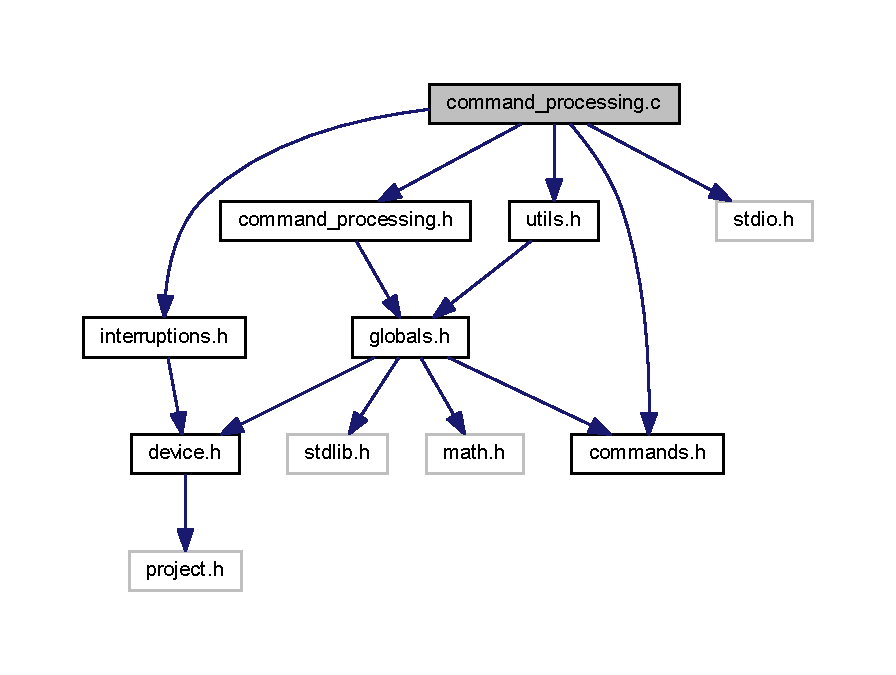
\includegraphics[width=350pt]{command__processing_8c__incl}
\end{center}
\end{figure}
\subsection*{Functions}
\begin{DoxyCompactItemize}
\item 
void \textbf{ comm\+Process} (void)
\item 
void \textbf{ info\+Send} (void)
\item 
void \textbf{ info\+Get} (uint16 info\+\_\+type)
\item 
void \textbf{ get\+\_\+param\+\_\+list} (uint16 index)
\item 
void \textbf{ set\+Zeros} ()
\item 
void \textbf{ info\+Prepare} (unsigned char $\ast$info\+\_\+string)
\item 
void \textbf{ comm\+Write\+\_\+old\+\_\+id} (uint8 $\ast$packet\+\_\+data, uint16 packet\+\_\+lenght, uint8 old\+\_\+id)
\item 
void \textbf{ comm\+Write} (uint8 $\ast$packet\+\_\+data, uint16 packet\+\_\+lenght)
\item 
int32 \textbf{ comm\+Read\+Meas\+From\+Another} ()
\item 
void \textbf{ comm\+Write\+Another} (uint8 $\ast$packet\+\_\+data, uint16 packet\+\_\+lenght)
\item 
uint8 \textbf{ L\+C\+R\+Checksum} (uint8 $\ast$data\+\_\+array, uint8 data\+\_\+length)
\item 
void \textbf{ send\+Acknowledgment} (uint8 value)
\item 
uint8 \textbf{ mem\+Store} (int displacement)
\item 
void \textbf{ mem\+Recall} (void)
\item 
uint8 \textbf{ mem\+Restore} (void)
\item 
uint8 \textbf{ mem\+Init} (void)
\item 
void \textbf{ cmd\+\_\+get\+\_\+measurements} ()
\item 
void \textbf{ cmd\+\_\+get\+\_\+measurements\+\_\+from\+\_\+\+SH} ()
\item 
void \textbf{ cmd\+\_\+set\+\_\+inputs} ()
\item 
void \textbf{ cmd\+\_\+activate} ()
\item 
void \textbf{ cmd\+\_\+get\+\_\+activate} ()
\item 
\mbox{\label{command__processing_8c_a45a90a8455bfdb6a7f0e118da2c6f0a6}} 
void {\bfseries cmd\+\_\+get\+\_\+curr\+\_\+and\+\_\+meas} ()
\item 
void \textbf{ cmd\+\_\+get\+\_\+currents} ()
\item 
void \textbf{ cmd\+\_\+set\+\_\+baudrate} ()
\item 
void \textbf{ cmd\+\_\+ping} ()
\item 
void \textbf{ cmd\+\_\+set\+\_\+watchdog} ()
\item 
void \textbf{ cmd\+\_\+get\+\_\+inputs} ()
\item 
void \textbf{ cmd\+\_\+store\+\_\+params} ()
\item 
void \textbf{ cmd\+\_\+get\+\_\+emg} ()
\end{DoxyCompactItemize}
\subsection*{Variables}
\begin{DoxyCompactItemize}
\item 
\mbox{\label{command__processing_8c_aba5b9353e6d38cc61eb2bd363df61248}} 
reg8 $\ast$ {\bfseries E\+E\+P\+R\+O\+M\+\_\+\+A\+D\+DR} = (reg8 $\ast$) C\+Y\+D\+E\+V\+\_\+\+E\+E\+\_\+\+B\+A\+SE
\end{DoxyCompactItemize}


\subsection{Detailed Description}
Command processing functions. 

\begin{DoxyDate}{Date}
October 01, 2017 
\end{DoxyDate}
\begin{DoxyAuthor}{Author}
{\itshape Centro \char`\"{}\+E.\+Piaggio\char`\"{}} 
\end{DoxyAuthor}
\begin{DoxyCopyright}{Copyright}
(C) 2012-\/2016 qbrobotics. All rights reserved. 

(C) 2017 Centro \char`\"{}\+E.\+Piaggio\char`\"{}. All rights reserved. 
\end{DoxyCopyright}


\subsection{Function Documentation}
\mbox{\label{command__processing_8c_a107fc9f2982f9a953bdd82aa07279499}} 
\index{command\+\_\+processing.\+c@{command\+\_\+processing.\+c}!cmd\+\_\+activate@{cmd\+\_\+activate}}
\index{cmd\+\_\+activate@{cmd\+\_\+activate}!command\+\_\+processing.\+c@{command\+\_\+processing.\+c}}
\subsubsection{cmd\+\_\+activate()}
{\footnotesize\ttfamily void cmd\+\_\+activate (\begin{DoxyParamCaption}{ }\end{DoxyParamCaption})}

This function activates the board \mbox{\label{command__processing_8c_a554d563001517bfbc44400a1e999b393}} 
\index{command\+\_\+processing.\+c@{command\+\_\+processing.\+c}!cmd\+\_\+get\+\_\+activate@{cmd\+\_\+get\+\_\+activate}}
\index{cmd\+\_\+get\+\_\+activate@{cmd\+\_\+get\+\_\+activate}!command\+\_\+processing.\+c@{command\+\_\+processing.\+c}}
\subsubsection{cmd\+\_\+get\+\_\+activate()}
{\footnotesize\ttfamily void cmd\+\_\+get\+\_\+activate (\begin{DoxyParamCaption}{ }\end{DoxyParamCaption})}

This function gets the board activation status and puts it in the package to be sent. \mbox{\label{command__processing_8c_aaf613e251c1e14fe4fffe3e9e033f9f7}} 
\index{command\+\_\+processing.\+c@{command\+\_\+processing.\+c}!cmd\+\_\+get\+\_\+currents@{cmd\+\_\+get\+\_\+currents}}
\index{cmd\+\_\+get\+\_\+currents@{cmd\+\_\+get\+\_\+currents}!command\+\_\+processing.\+c@{command\+\_\+processing.\+c}}
\subsubsection{cmd\+\_\+get\+\_\+currents()}
{\footnotesize\ttfamily void cmd\+\_\+get\+\_\+currents (\begin{DoxyParamCaption}{ }\end{DoxyParamCaption})}

This function gets the motor current and puts it in the package to be sent. \mbox{\label{command__processing_8c_ae579c6ac56fef33632f9c9f2c42b90a0}} 
\index{command\+\_\+processing.\+c@{command\+\_\+processing.\+c}!cmd\+\_\+get\+\_\+emg@{cmd\+\_\+get\+\_\+emg}}
\index{cmd\+\_\+get\+\_\+emg@{cmd\+\_\+get\+\_\+emg}!command\+\_\+processing.\+c@{command\+\_\+processing.\+c}}
\subsubsection{cmd\+\_\+get\+\_\+emg()}
{\footnotesize\ttfamily void cmd\+\_\+get\+\_\+emg (\begin{DoxyParamCaption}{ }\end{DoxyParamCaption})}

This function gets the electromyographic sensors measurements and puts them in the package to be sent. \mbox{\label{command__processing_8c_a20db4694e8caa572ec479f73ce8b3b02}} 
\index{command\+\_\+processing.\+c@{command\+\_\+processing.\+c}!cmd\+\_\+get\+\_\+inputs@{cmd\+\_\+get\+\_\+inputs}}
\index{cmd\+\_\+get\+\_\+inputs@{cmd\+\_\+get\+\_\+inputs}!command\+\_\+processing.\+c@{command\+\_\+processing.\+c}}
\subsubsection{cmd\+\_\+get\+\_\+inputs()}
{\footnotesize\ttfamily void cmd\+\_\+get\+\_\+inputs (\begin{DoxyParamCaption}{ }\end{DoxyParamCaption})}

This function gets the current motor reference inputs and puts them in the package to be sent. \mbox{\label{command__processing_8c_af5ccd403f1d3e49c97bafd6e7713cff3}} 
\index{command\+\_\+processing.\+c@{command\+\_\+processing.\+c}!cmd\+\_\+get\+\_\+measurements@{cmd\+\_\+get\+\_\+measurements}}
\index{cmd\+\_\+get\+\_\+measurements@{cmd\+\_\+get\+\_\+measurements}!command\+\_\+processing.\+c@{command\+\_\+processing.\+c}}
\subsubsection{cmd\+\_\+get\+\_\+measurements()}
{\footnotesize\ttfamily void cmd\+\_\+get\+\_\+measurements (\begin{DoxyParamCaption}{ }\end{DoxyParamCaption})}

Bunch of functions used on request from U\+A\+RT communication \mbox{\label{command__processing_8c_ad44d76176312ce9391dbb857f75a3595}} 
\index{command\+\_\+processing.\+c@{command\+\_\+processing.\+c}!cmd\+\_\+get\+\_\+measurements\+\_\+from\+\_\+\+SH@{cmd\+\_\+get\+\_\+measurements\+\_\+from\+\_\+\+SH}}
\index{cmd\+\_\+get\+\_\+measurements\+\_\+from\+\_\+\+SH@{cmd\+\_\+get\+\_\+measurements\+\_\+from\+\_\+\+SH}!command\+\_\+processing.\+c@{command\+\_\+processing.\+c}}
\subsubsection{cmd\+\_\+get\+\_\+measurements\+\_\+from\+\_\+\+S\+H()}
{\footnotesize\ttfamily void cmd\+\_\+get\+\_\+measurements\+\_\+from\+\_\+\+SH (\begin{DoxyParamCaption}{ }\end{DoxyParamCaption})}

This function gets the encoders measurements from SH in master mode and puts them in the package to be sent. \mbox{\label{command__processing_8c_a704f8c8cb0f4d75f243fc2b79bc34188}} 
\index{command\+\_\+processing.\+c@{command\+\_\+processing.\+c}!cmd\+\_\+ping@{cmd\+\_\+ping}}
\index{cmd\+\_\+ping@{cmd\+\_\+ping}!command\+\_\+processing.\+c@{command\+\_\+processing.\+c}}
\subsubsection{cmd\+\_\+ping()}
{\footnotesize\ttfamily void cmd\+\_\+ping (\begin{DoxyParamCaption}{ }\end{DoxyParamCaption})}

This function is used to ping the device and see if is connected. \mbox{\label{command__processing_8c_aa86bf1f2fa69ab5927f7e4e40eb40581}} 
\index{command\+\_\+processing.\+c@{command\+\_\+processing.\+c}!cmd\+\_\+set\+\_\+baudrate@{cmd\+\_\+set\+\_\+baudrate}}
\index{cmd\+\_\+set\+\_\+baudrate@{cmd\+\_\+set\+\_\+baudrate}!command\+\_\+processing.\+c@{command\+\_\+processing.\+c}}
\subsubsection{cmd\+\_\+set\+\_\+baudrate()}
{\footnotesize\ttfamily void cmd\+\_\+set\+\_\+baudrate (\begin{DoxyParamCaption}{ }\end{DoxyParamCaption})}

This function sets the desired communication baudrate. It is possible to select a value equal to 460800 or 2000000. \mbox{\label{command__processing_8c_a2d8a4542f55af960a27f875b00aad6a1}} 
\index{command\+\_\+processing.\+c@{command\+\_\+processing.\+c}!cmd\+\_\+set\+\_\+inputs@{cmd\+\_\+set\+\_\+inputs}}
\index{cmd\+\_\+set\+\_\+inputs@{cmd\+\_\+set\+\_\+inputs}!command\+\_\+processing.\+c@{command\+\_\+processing.\+c}}
\subsubsection{cmd\+\_\+set\+\_\+inputs()}
{\footnotesize\ttfamily void cmd\+\_\+set\+\_\+inputs (\begin{DoxyParamCaption}{ }\end{DoxyParamCaption})}

This function gets the inputs from the received package and sets them as motor reference. \mbox{\label{command__processing_8c_aa94cd9c2e2fbfc5b98e84f67569cfe82}} 
\index{command\+\_\+processing.\+c@{command\+\_\+processing.\+c}!cmd\+\_\+set\+\_\+watchdog@{cmd\+\_\+set\+\_\+watchdog}}
\index{cmd\+\_\+set\+\_\+watchdog@{cmd\+\_\+set\+\_\+watchdog}!command\+\_\+processing.\+c@{command\+\_\+processing.\+c}}
\subsubsection{cmd\+\_\+set\+\_\+watchdog()}
{\footnotesize\ttfamily void cmd\+\_\+set\+\_\+watchdog (\begin{DoxyParamCaption}{ }\end{DoxyParamCaption})}

This function sets the watchdog timer to the one received from the package. The board automatically deactivate when the time equivalent, to watchdog timer, has passed. \mbox{\label{command__processing_8c_a1a2493bfc2f30171d7e7a3bd5aebab14}} 
\index{command\+\_\+processing.\+c@{command\+\_\+processing.\+c}!cmd\+\_\+store\+\_\+params@{cmd\+\_\+store\+\_\+params}}
\index{cmd\+\_\+store\+\_\+params@{cmd\+\_\+store\+\_\+params}!command\+\_\+processing.\+c@{command\+\_\+processing.\+c}}
\subsubsection{cmd\+\_\+store\+\_\+params()}
{\footnotesize\ttfamily void cmd\+\_\+store\+\_\+params (\begin{DoxyParamCaption}{ }\end{DoxyParamCaption})}

This function stores the parameters to the E\+E\+P\+R\+OM memory \mbox{\label{command__processing_8c_a0c97206a61d782ebd9aa24bbb96f8aea}} 
\index{command\+\_\+processing.\+c@{command\+\_\+processing.\+c}!comm\+Process@{comm\+Process}}
\index{comm\+Process@{comm\+Process}!command\+\_\+processing.\+c@{command\+\_\+processing.\+c}}
\subsubsection{comm\+Process()}
{\footnotesize\ttfamily void comm\+Process (\begin{DoxyParamCaption}{ }\end{DoxyParamCaption})}

This function unpacks the received package, depending on the command received. \mbox{\label{command__processing_8c_a61d4e075c64c8b4b79bfadfce576d357}} 
\index{command\+\_\+processing.\+c@{command\+\_\+processing.\+c}!comm\+Read\+Meas\+From\+Another@{comm\+Read\+Meas\+From\+Another}}
\index{comm\+Read\+Meas\+From\+Another@{comm\+Read\+Meas\+From\+Another}!command\+\_\+processing.\+c@{command\+\_\+processing.\+c}}
\subsubsection{comm\+Read\+Meas\+From\+Another()}
{\footnotesize\ttfamily int32 comm\+Read\+Meas\+From\+Another (\begin{DoxyParamCaption}{ }\end{DoxyParamCaption})}

This function reads on the serial port the measurements package from another board. \mbox{\label{command__processing_8c_af92ab4f3c1e0c0e8f5966bf2e2edeaba}} 
\index{command\+\_\+processing.\+c@{command\+\_\+processing.\+c}!comm\+Write@{comm\+Write}}
\index{comm\+Write@{comm\+Write}!command\+\_\+processing.\+c@{command\+\_\+processing.\+c}}
\subsubsection{comm\+Write()}
{\footnotesize\ttfamily void comm\+Write (\begin{DoxyParamCaption}\item[{uint8 $\ast$}]{packet\+\_\+data,  }\item[{uint16}]{packet\+\_\+lenght }\end{DoxyParamCaption})}

This function writes on the serial port the package that needs to be sent to the user.


\begin{DoxyParams}{Parameters}
{\em packet\+\_\+data} & The array of data that must be written. \\
\hline
{\em packet\+\_\+lenght} & The lenght of the data array. \\
\hline
\end{DoxyParams}
\mbox{\label{command__processing_8c_a517f4c61166381d40767fce9011e3c96}} 
\index{command\+\_\+processing.\+c@{command\+\_\+processing.\+c}!comm\+Write\+\_\+old\+\_\+id@{comm\+Write\+\_\+old\+\_\+id}}
\index{comm\+Write\+\_\+old\+\_\+id@{comm\+Write\+\_\+old\+\_\+id}!command\+\_\+processing.\+c@{command\+\_\+processing.\+c}}
\subsubsection{comm\+Write\+\_\+old\+\_\+id()}
{\footnotesize\ttfamily void comm\+Write\+\_\+old\+\_\+id (\begin{DoxyParamCaption}\item[{uint8 $\ast$}]{packet\+\_\+data,  }\item[{uint16}]{packet\+\_\+lenght,  }\item[{uint8}]{old\+\_\+id }\end{DoxyParamCaption})}

This function writes on the serial port the package that needs to be sent to the user. Is used only when a new is set, to communicate back to the A\+P\+Is that the new ID setting went fine or there was an error.


\begin{DoxyParams}{Parameters}
{\em packet\+\_\+data} & The array of data that must be written. \\
\hline
{\em packet\+\_\+lenght} & The lenght of the data array. \\
\hline
{\em old\+\_\+id} & The previous id of the board, before setting a new one \\
\hline
\end{DoxyParams}
\mbox{\label{command__processing_8c_ab8e39f8e58dc9f567f24291b11b4d8d0}} 
\index{command\+\_\+processing.\+c@{command\+\_\+processing.\+c}!comm\+Write\+Another@{comm\+Write\+Another}}
\index{comm\+Write\+Another@{comm\+Write\+Another}!command\+\_\+processing.\+c@{command\+\_\+processing.\+c}}
\subsubsection{comm\+Write\+Another()}
{\footnotesize\ttfamily void comm\+Write\+Another (\begin{DoxyParamCaption}\item[{uint8 $\ast$}]{packet\+\_\+data,  }\item[{uint16}]{packet\+\_\+lenght }\end{DoxyParamCaption})}

This function writes on the serial port the package that needs to be sent to another board.


\begin{DoxyParams}{Parameters}
{\em packet\+\_\+data} & The array of data that must be written. \\
\hline
{\em packet\+\_\+lenght} & The lenght of the data array. \\
\hline
\end{DoxyParams}
\mbox{\label{command__processing_8c_a5ef086c932682ca5f7549b74ead732aa}} 
\index{command\+\_\+processing.\+c@{command\+\_\+processing.\+c}!get\+\_\+param\+\_\+list@{get\+\_\+param\+\_\+list}}
\index{get\+\_\+param\+\_\+list@{get\+\_\+param\+\_\+list}!command\+\_\+processing.\+c@{command\+\_\+processing.\+c}}
\subsubsection{get\+\_\+param\+\_\+list()}
{\footnotesize\ttfamily void get\+\_\+param\+\_\+list (\begin{DoxyParamCaption}\item[{uint16}]{index }\end{DoxyParamCaption})}

This function, depending on the \doxyref{Firmware}{p.}{index} received, gets the list of parameters with their values and sends them to user or sets a parameter from all the parameters of the device.


\begin{DoxyParams}{Parameters}
{\em index} & The index of the parameters to be setted. If 0 gets full parameters list. \\
\hline
\end{DoxyParams}
\mbox{\label{command__processing_8c_a525ccbc7ac3901d938dc352172ee2531}} 
\index{command\+\_\+processing.\+c@{command\+\_\+processing.\+c}!info\+Get@{info\+Get}}
\index{info\+Get@{info\+Get}!command\+\_\+processing.\+c@{command\+\_\+processing.\+c}}
\subsubsection{info\+Get()}
{\footnotesize\ttfamily void info\+Get (\begin{DoxyParamCaption}\item[{uint16}]{info\+\_\+type }\end{DoxyParamCaption})}

This function sends the firmware information prepared with \doxyref{info\+Prepare}{p.}{command__processing_8h_abacf855ed80e3052a5bb5b243a0d809e} through the serial port to the user interface. Is used when the ID is specified.


\begin{DoxyParams}{Parameters}
{\em info\+\_\+type} & The type of the information needed. \\
\hline
\end{DoxyParams}
\mbox{\label{command__processing_8c_abacf855ed80e3052a5bb5b243a0d809e}} 
\index{command\+\_\+processing.\+c@{command\+\_\+processing.\+c}!info\+Prepare@{info\+Prepare}}
\index{info\+Prepare@{info\+Prepare}!command\+\_\+processing.\+c@{command\+\_\+processing.\+c}}
\subsubsection{info\+Prepare()}
{\footnotesize\ttfamily void info\+Prepare (\begin{DoxyParamCaption}\item[{unsigned char $\ast$}]{info\+\_\+string }\end{DoxyParamCaption})}

This function is used to prepare the information string about the firmware of the device.


\begin{DoxyParams}{Parameters}
{\em info\+\_\+string} & An array of chars containing firmware informations. \\
\hline
\end{DoxyParams}
\mbox{\label{command__processing_8c_a0f8a936c0c43abd1e7ba5add8cbcbf70}} 
\index{command\+\_\+processing.\+c@{command\+\_\+processing.\+c}!info\+Send@{info\+Send}}
\index{info\+Send@{info\+Send}!command\+\_\+processing.\+c@{command\+\_\+processing.\+c}}
\subsubsection{info\+Send()}
{\footnotesize\ttfamily void info\+Send (\begin{DoxyParamCaption}{ }\end{DoxyParamCaption})}

This function sends the firmware information prepared with \doxyref{info\+Prepare}{p.}{command__processing_8h_abacf855ed80e3052a5bb5b243a0d809e} through the serial port to the user interface. Is used when no ID is specified. \mbox{\label{command__processing_8c_a6205a6e88f72f4cc321a7d8abca23e26}} 
\index{command\+\_\+processing.\+c@{command\+\_\+processing.\+c}!L\+C\+R\+Checksum@{L\+C\+R\+Checksum}}
\index{L\+C\+R\+Checksum@{L\+C\+R\+Checksum}!command\+\_\+processing.\+c@{command\+\_\+processing.\+c}}
\subsubsection{L\+C\+R\+Checksum()}
{\footnotesize\ttfamily uint8 L\+C\+R\+Checksum (\begin{DoxyParamCaption}\item[{uint8 $\ast$}]{data\+\_\+array,  }\item[{uint8}]{data\+\_\+length }\end{DoxyParamCaption})}

This function calculates a checksum of the array to see if the received data is consistent.


\begin{DoxyParams}{Parameters}
{\em data\+\_\+array} & The array of data that must be checked. \\
\hline
{\em data\+\_\+lenght} & Lenght of the data array that must be checked.\\
\hline
\end{DoxyParams}
\begin{DoxyReturn}{Returns}
The calculated checksum for the relative data\+\_\+array. 
\end{DoxyReturn}
\mbox{\label{command__processing_8c_a48f1d2aa212e255d0a3322e576fc8574}} 
\index{command\+\_\+processing.\+c@{command\+\_\+processing.\+c}!mem\+Init@{mem\+Init}}
\index{mem\+Init@{mem\+Init}!command\+\_\+processing.\+c@{command\+\_\+processing.\+c}}
\subsubsection{mem\+Init()}
{\footnotesize\ttfamily uint8 mem\+Init (\begin{DoxyParamCaption}{ }\end{DoxyParamCaption})}

This functions initializes the memory. It is used also to restore the the parameters to their default values.

\begin{DoxyReturn}{Returns}
A true value if the memory is correctly initialized, false otherwise. 
\end{DoxyReturn}
\mbox{\label{command__processing_8c_a494f1f72ae370f0057e5aa3db73ef6fb}} 
\index{command\+\_\+processing.\+c@{command\+\_\+processing.\+c}!mem\+Recall@{mem\+Recall}}
\index{mem\+Recall@{mem\+Recall}!command\+\_\+processing.\+c@{command\+\_\+processing.\+c}}
\subsubsection{mem\+Recall()}
{\footnotesize\ttfamily void mem\+Recall (\begin{DoxyParamCaption}{ }\end{DoxyParamCaption})}

This function loads user\textquotesingle{}s settings from the E\+E\+P\+R\+OM. \mbox{\label{command__processing_8c_af67845c368ea7fefb79a1f0baa12134c}} 
\index{command\+\_\+processing.\+c@{command\+\_\+processing.\+c}!mem\+Restore@{mem\+Restore}}
\index{mem\+Restore@{mem\+Restore}!command\+\_\+processing.\+c@{command\+\_\+processing.\+c}}
\subsubsection{mem\+Restore()}
{\footnotesize\ttfamily uint8 mem\+Restore (\begin{DoxyParamCaption}{ }\end{DoxyParamCaption})}

This function loads default settings from the E\+E\+P\+R\+OM.

\begin{DoxyReturn}{Returns}
A true value if the memory is correctly restored, false otherwise. 
\end{DoxyReturn}
\mbox{\label{command__processing_8c_a81e6b73c0ee52661736a97c08bdb262b}} 
\index{command\+\_\+processing.\+c@{command\+\_\+processing.\+c}!mem\+Store@{mem\+Store}}
\index{mem\+Store@{mem\+Store}!command\+\_\+processing.\+c@{command\+\_\+processing.\+c}}
\subsubsection{mem\+Store()}
{\footnotesize\ttfamily uint8 mem\+Store (\begin{DoxyParamCaption}\item[{int}]{displacement }\end{DoxyParamCaption})}

This function stores the setted parameters to the internal E\+E\+P\+R\+OM memory. It is usually called, by the user, after a parameter is set.


\begin{DoxyParams}{Parameters}
{\em displacement} & The address where the parameters will be written.\\
\hline
\end{DoxyParams}
\begin{DoxyReturn}{Returns}
A true value if the memory is correctly stored, false otherwise. 
\end{DoxyReturn}
\mbox{\label{command__processing_8c_a1a2eafee01079c42ca1fb14aa7331933}} 
\index{command\+\_\+processing.\+c@{command\+\_\+processing.\+c}!send\+Acknowledgment@{send\+Acknowledgment}}
\index{send\+Acknowledgment@{send\+Acknowledgment}!command\+\_\+processing.\+c@{command\+\_\+processing.\+c}}
\subsubsection{send\+Acknowledgment()}
{\footnotesize\ttfamily void send\+Acknowledgment (\begin{DoxyParamCaption}\item[{uint8}]{value }\end{DoxyParamCaption})}

This functions sends an acknowledgment to see if a command has been executed properly or not.


\begin{DoxyParams}{Parameters}
{\em value} & An A\+C\+K\+\_\+\+O\+K(1) or A\+C\+K\+\_\+\+E\+R\+R\+O\+R(0) value. \\
\hline
\end{DoxyParams}
\mbox{\label{command__processing_8c_ac8969cb5fdb4916f259075029741e727}} 
\index{command\+\_\+processing.\+c@{command\+\_\+processing.\+c}!set\+Zeros@{set\+Zeros}}
\index{set\+Zeros@{set\+Zeros}!command\+\_\+processing.\+c@{command\+\_\+processing.\+c}}
\subsubsection{set\+Zeros()}
{\footnotesize\ttfamily void set\+Zeros (\begin{DoxyParamCaption}{ }\end{DoxyParamCaption})}

This function sets the encoders zero position. 
\section{command\+\_\+processing.\+h File Reference}
\label{command__processing_8h}\index{command\+\_\+processing.\+h@{command\+\_\+processing.\+h}}


Received commands processing functions.  


{\ttfamily \#include $<$globals.\+h$>$}\newline
Include dependency graph for command\+\_\+processing.\+h\+:
\nopagebreak
\begin{figure}[H]
\begin{center}
\leavevmode
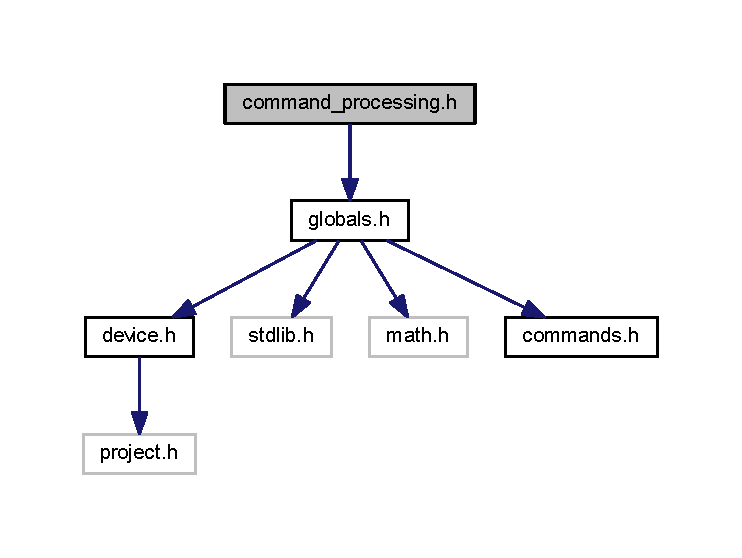
\includegraphics[width=350pt]{command__processing_8h__incl}
\end{center}
\end{figure}
This graph shows which files directly or indirectly include this file\+:\nopagebreak
\begin{figure}[H]
\begin{center}
\leavevmode
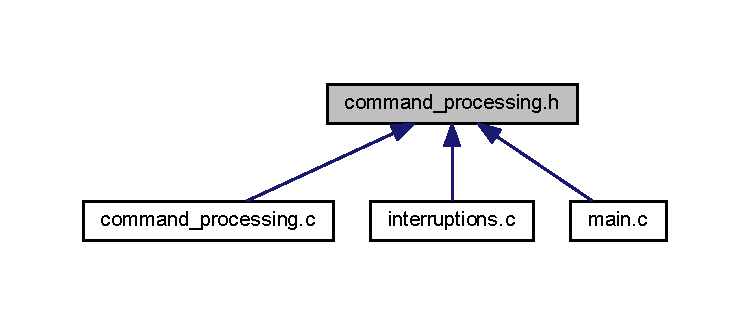
\includegraphics[width=350pt]{command__processing_8h__dep__incl}
\end{center}
\end{figure}
\subsection*{Functions}
\begin{Indent}\textbf{ Firmware information functions}\par
\begin{DoxyCompactItemize}
\item 
void \textbf{ info\+Prepare} (unsigned char $\ast$info\+\_\+string)
\item 
void \textbf{ info\+Send} ()
\item 
void \textbf{ info\+Get} (uint16 info\+\_\+type)
\end{DoxyCompactItemize}
\end{Indent}
\begin{Indent}\textbf{ Command receiving and sending functions}\par
\begin{DoxyCompactItemize}
\item 
void \textbf{ comm\+Process} ()
\item 
void \textbf{ comm\+Write\+\_\+old\+\_\+id} (uint8 $\ast$packet\+\_\+data, uint16 packet\+\_\+lenght, uint8 old\+\_\+id)
\item 
void \textbf{ comm\+Write} (uint8 $\ast$packet\+\_\+data, uint16 packet\+\_\+lenght)
\item 
void \textbf{ comm\+Write\+Another} (uint8 $\ast$packet\+\_\+data, uint16 packet\+\_\+lenght)
\item 
int32 \textbf{ comm\+Read\+Meas\+From\+Another} ()
\end{DoxyCompactItemize}
\end{Indent}
\begin{Indent}\textbf{ Memory management functions}\par
\begin{DoxyCompactItemize}
\item 
void \textbf{ get\+\_\+param\+\_\+list} (uint16 index)
\item 
void \textbf{ set\+Zeros} ()
\item 
uint8 \textbf{ mem\+Store} (int displacement)
\item 
void \textbf{ mem\+Recall} ()
\item 
uint8 \textbf{ mem\+Restore} ()
\item 
uint8 \textbf{ mem\+Init} ()
\end{DoxyCompactItemize}
\end{Indent}
\begin{Indent}\textbf{ Utility functions}\par
\begin{DoxyCompactItemize}
\item 
uint8 \textbf{ L\+C\+R\+Checksum} (uint8 $\ast$data\+\_\+array, uint8 data\+\_\+length)
\item 
void \textbf{ send\+Acknowledgment} (uint8 value)
\end{DoxyCompactItemize}
\end{Indent}
\begin{Indent}\textbf{ Command processing functions}\par
\begin{DoxyCompactItemize}
\item 
void \textbf{ cmd\+\_\+activate} ()
\item 
void \textbf{ cmd\+\_\+set\+\_\+inputs} ()
\item 
void \textbf{ cmd\+\_\+get\+\_\+measurements} ()
\item 
void \textbf{ cmd\+\_\+get\+\_\+measurements\+\_\+from\+\_\+\+SH} ()
\item 
void \textbf{ cmd\+\_\+get\+\_\+currents} ()
\item 
void \textbf{ cmd\+\_\+get\+\_\+emg} ()
\item 
void \textbf{ cmd\+\_\+set\+\_\+watchdog} ()
\item 
void \textbf{ cmd\+\_\+get\+\_\+activate} ()
\item 
void \textbf{ cmd\+\_\+set\+\_\+baudrate} ()
\item 
void \textbf{ cmd\+\_\+get\+\_\+inputs} ()
\item 
void \textbf{ cmd\+\_\+store\+\_\+params} ()
\item 
void \textbf{ cmd\+\_\+ping} ()
\end{DoxyCompactItemize}
\end{Indent}


\subsection{Detailed Description}
Received commands processing functions. 

\begin{DoxyDate}{Date}
October 01, 2017 
\end{DoxyDate}
\begin{DoxyAuthor}{Author}
{\itshape Centro \char`\"{}\+E.\+Piaggio\char`\"{}} 
\end{DoxyAuthor}
\begin{DoxyCopyright}{Copyright}
(C) 2012-\/2016 qbrobotics. All rights reserved. 

(C) 2017 Centro \char`\"{}\+E.\+Piaggio\char`\"{}. All rights reserved.
\end{DoxyCopyright}
This file contains all the definitions of the functions used to process the commands sent from the user interfaces (simulink, command line, G\+UI) 

\subsection{Function Documentation}
\mbox{\label{command__processing_8h_a107fc9f2982f9a953bdd82aa07279499}} 
\index{command\+\_\+processing.\+h@{command\+\_\+processing.\+h}!cmd\+\_\+activate@{cmd\+\_\+activate}}
\index{cmd\+\_\+activate@{cmd\+\_\+activate}!command\+\_\+processing.\+h@{command\+\_\+processing.\+h}}
\subsubsection{cmd\+\_\+activate()}
{\footnotesize\ttfamily void cmd\+\_\+activate (\begin{DoxyParamCaption}{ }\end{DoxyParamCaption})}

This function activates the board \mbox{\label{command__processing_8h_a554d563001517bfbc44400a1e999b393}} 
\index{command\+\_\+processing.\+h@{command\+\_\+processing.\+h}!cmd\+\_\+get\+\_\+activate@{cmd\+\_\+get\+\_\+activate}}
\index{cmd\+\_\+get\+\_\+activate@{cmd\+\_\+get\+\_\+activate}!command\+\_\+processing.\+h@{command\+\_\+processing.\+h}}
\subsubsection{cmd\+\_\+get\+\_\+activate()}
{\footnotesize\ttfamily void cmd\+\_\+get\+\_\+activate (\begin{DoxyParamCaption}{ }\end{DoxyParamCaption})}

This function gets the board activation status and puts it in the package to be sent. \mbox{\label{command__processing_8h_aaf613e251c1e14fe4fffe3e9e033f9f7}} 
\index{command\+\_\+processing.\+h@{command\+\_\+processing.\+h}!cmd\+\_\+get\+\_\+currents@{cmd\+\_\+get\+\_\+currents}}
\index{cmd\+\_\+get\+\_\+currents@{cmd\+\_\+get\+\_\+currents}!command\+\_\+processing.\+h@{command\+\_\+processing.\+h}}
\subsubsection{cmd\+\_\+get\+\_\+currents()}
{\footnotesize\ttfamily void cmd\+\_\+get\+\_\+currents (\begin{DoxyParamCaption}{ }\end{DoxyParamCaption})}

This function gets the motor current and puts it in the package to be sent. \mbox{\label{command__processing_8h_ae579c6ac56fef33632f9c9f2c42b90a0}} 
\index{command\+\_\+processing.\+h@{command\+\_\+processing.\+h}!cmd\+\_\+get\+\_\+emg@{cmd\+\_\+get\+\_\+emg}}
\index{cmd\+\_\+get\+\_\+emg@{cmd\+\_\+get\+\_\+emg}!command\+\_\+processing.\+h@{command\+\_\+processing.\+h}}
\subsubsection{cmd\+\_\+get\+\_\+emg()}
{\footnotesize\ttfamily void cmd\+\_\+get\+\_\+emg (\begin{DoxyParamCaption}{ }\end{DoxyParamCaption})}

This function gets the electromyographic sensors measurements and puts them in the package to be sent. \mbox{\label{command__processing_8h_a20db4694e8caa572ec479f73ce8b3b02}} 
\index{command\+\_\+processing.\+h@{command\+\_\+processing.\+h}!cmd\+\_\+get\+\_\+inputs@{cmd\+\_\+get\+\_\+inputs}}
\index{cmd\+\_\+get\+\_\+inputs@{cmd\+\_\+get\+\_\+inputs}!command\+\_\+processing.\+h@{command\+\_\+processing.\+h}}
\subsubsection{cmd\+\_\+get\+\_\+inputs()}
{\footnotesize\ttfamily void cmd\+\_\+get\+\_\+inputs (\begin{DoxyParamCaption}{ }\end{DoxyParamCaption})}

This function gets the current motor reference inputs and puts them in the package to be sent. \mbox{\label{command__processing_8h_af5ccd403f1d3e49c97bafd6e7713cff3}} 
\index{command\+\_\+processing.\+h@{command\+\_\+processing.\+h}!cmd\+\_\+get\+\_\+measurements@{cmd\+\_\+get\+\_\+measurements}}
\index{cmd\+\_\+get\+\_\+measurements@{cmd\+\_\+get\+\_\+measurements}!command\+\_\+processing.\+h@{command\+\_\+processing.\+h}}
\subsubsection{cmd\+\_\+get\+\_\+measurements()}
{\footnotesize\ttfamily void cmd\+\_\+get\+\_\+measurements (\begin{DoxyParamCaption}{ }\end{DoxyParamCaption})}

This function gets the encoders measurements and puts them in the package to be sent.

Bunch of functions used on request from U\+A\+RT communication \mbox{\label{command__processing_8h_ad44d76176312ce9391dbb857f75a3595}} 
\index{command\+\_\+processing.\+h@{command\+\_\+processing.\+h}!cmd\+\_\+get\+\_\+measurements\+\_\+from\+\_\+\+SH@{cmd\+\_\+get\+\_\+measurements\+\_\+from\+\_\+\+SH}}
\index{cmd\+\_\+get\+\_\+measurements\+\_\+from\+\_\+\+SH@{cmd\+\_\+get\+\_\+measurements\+\_\+from\+\_\+\+SH}!command\+\_\+processing.\+h@{command\+\_\+processing.\+h}}
\subsubsection{cmd\+\_\+get\+\_\+measurements\+\_\+from\+\_\+\+S\+H()}
{\footnotesize\ttfamily void cmd\+\_\+get\+\_\+measurements\+\_\+from\+\_\+\+SH (\begin{DoxyParamCaption}{ }\end{DoxyParamCaption})}

This function gets the encoders measurements from SH in master mode and puts them in the package to be sent. \mbox{\label{command__processing_8h_a704f8c8cb0f4d75f243fc2b79bc34188}} 
\index{command\+\_\+processing.\+h@{command\+\_\+processing.\+h}!cmd\+\_\+ping@{cmd\+\_\+ping}}
\index{cmd\+\_\+ping@{cmd\+\_\+ping}!command\+\_\+processing.\+h@{command\+\_\+processing.\+h}}
\subsubsection{cmd\+\_\+ping()}
{\footnotesize\ttfamily void cmd\+\_\+ping (\begin{DoxyParamCaption}{ }\end{DoxyParamCaption})}

This function is used to ping the device and see if is connected. \mbox{\label{command__processing_8h_aa86bf1f2fa69ab5927f7e4e40eb40581}} 
\index{command\+\_\+processing.\+h@{command\+\_\+processing.\+h}!cmd\+\_\+set\+\_\+baudrate@{cmd\+\_\+set\+\_\+baudrate}}
\index{cmd\+\_\+set\+\_\+baudrate@{cmd\+\_\+set\+\_\+baudrate}!command\+\_\+processing.\+h@{command\+\_\+processing.\+h}}
\subsubsection{cmd\+\_\+set\+\_\+baudrate()}
{\footnotesize\ttfamily void cmd\+\_\+set\+\_\+baudrate (\begin{DoxyParamCaption}{ }\end{DoxyParamCaption})}

This function sets the desired communication baudrate. It is possible to select a value equal to 460800 or 2000000. \mbox{\label{command__processing_8h_a2d8a4542f55af960a27f875b00aad6a1}} 
\index{command\+\_\+processing.\+h@{command\+\_\+processing.\+h}!cmd\+\_\+set\+\_\+inputs@{cmd\+\_\+set\+\_\+inputs}}
\index{cmd\+\_\+set\+\_\+inputs@{cmd\+\_\+set\+\_\+inputs}!command\+\_\+processing.\+h@{command\+\_\+processing.\+h}}
\subsubsection{cmd\+\_\+set\+\_\+inputs()}
{\footnotesize\ttfamily void cmd\+\_\+set\+\_\+inputs (\begin{DoxyParamCaption}{ }\end{DoxyParamCaption})}

This function gets the inputs from the received package and sets them as motor reference. \mbox{\label{command__processing_8h_aa94cd9c2e2fbfc5b98e84f67569cfe82}} 
\index{command\+\_\+processing.\+h@{command\+\_\+processing.\+h}!cmd\+\_\+set\+\_\+watchdog@{cmd\+\_\+set\+\_\+watchdog}}
\index{cmd\+\_\+set\+\_\+watchdog@{cmd\+\_\+set\+\_\+watchdog}!command\+\_\+processing.\+h@{command\+\_\+processing.\+h}}
\subsubsection{cmd\+\_\+set\+\_\+watchdog()}
{\footnotesize\ttfamily void cmd\+\_\+set\+\_\+watchdog (\begin{DoxyParamCaption}{ }\end{DoxyParamCaption})}

This function sets the watchdog timer to the one received from the package. The board automatically deactivate when the time equivalent, to watchdog timer, has passed. \mbox{\label{command__processing_8h_a1a2493bfc2f30171d7e7a3bd5aebab14}} 
\index{command\+\_\+processing.\+h@{command\+\_\+processing.\+h}!cmd\+\_\+store\+\_\+params@{cmd\+\_\+store\+\_\+params}}
\index{cmd\+\_\+store\+\_\+params@{cmd\+\_\+store\+\_\+params}!command\+\_\+processing.\+h@{command\+\_\+processing.\+h}}
\subsubsection{cmd\+\_\+store\+\_\+params()}
{\footnotesize\ttfamily void cmd\+\_\+store\+\_\+params (\begin{DoxyParamCaption}{ }\end{DoxyParamCaption})}

This function stores the parameters to the E\+E\+P\+R\+OM memory \mbox{\label{command__processing_8h_a2e5d1711e19837adc3e8f479af3ae509}} 
\index{command\+\_\+processing.\+h@{command\+\_\+processing.\+h}!comm\+Process@{comm\+Process}}
\index{comm\+Process@{comm\+Process}!command\+\_\+processing.\+h@{command\+\_\+processing.\+h}}
\subsubsection{comm\+Process()}
{\footnotesize\ttfamily void comm\+Process (\begin{DoxyParamCaption}{ }\end{DoxyParamCaption})}

This function unpacks the received package, depending on the command received. \mbox{\label{command__processing_8h_a61d4e075c64c8b4b79bfadfce576d357}} 
\index{command\+\_\+processing.\+h@{command\+\_\+processing.\+h}!comm\+Read\+Meas\+From\+Another@{comm\+Read\+Meas\+From\+Another}}
\index{comm\+Read\+Meas\+From\+Another@{comm\+Read\+Meas\+From\+Another}!command\+\_\+processing.\+h@{command\+\_\+processing.\+h}}
\subsubsection{comm\+Read\+Meas\+From\+Another()}
{\footnotesize\ttfamily int32 comm\+Read\+Meas\+From\+Another (\begin{DoxyParamCaption}{ }\end{DoxyParamCaption})}

This function reads on the serial port the measurements package from another board. \mbox{\label{command__processing_8h_af92ab4f3c1e0c0e8f5966bf2e2edeaba}} 
\index{command\+\_\+processing.\+h@{command\+\_\+processing.\+h}!comm\+Write@{comm\+Write}}
\index{comm\+Write@{comm\+Write}!command\+\_\+processing.\+h@{command\+\_\+processing.\+h}}
\subsubsection{comm\+Write()}
{\footnotesize\ttfamily void comm\+Write (\begin{DoxyParamCaption}\item[{uint8 $\ast$}]{packet\+\_\+data,  }\item[{uint16}]{packet\+\_\+lenght }\end{DoxyParamCaption})}

This function writes on the serial port the package that needs to be sent to the user.


\begin{DoxyParams}{Parameters}
{\em packet\+\_\+data} & The array of data that must be written. \\
\hline
{\em packet\+\_\+lenght} & The lenght of the data array. \\
\hline
\end{DoxyParams}
\mbox{\label{command__processing_8h_a517f4c61166381d40767fce9011e3c96}} 
\index{command\+\_\+processing.\+h@{command\+\_\+processing.\+h}!comm\+Write\+\_\+old\+\_\+id@{comm\+Write\+\_\+old\+\_\+id}}
\index{comm\+Write\+\_\+old\+\_\+id@{comm\+Write\+\_\+old\+\_\+id}!command\+\_\+processing.\+h@{command\+\_\+processing.\+h}}
\subsubsection{comm\+Write\+\_\+old\+\_\+id()}
{\footnotesize\ttfamily void comm\+Write\+\_\+old\+\_\+id (\begin{DoxyParamCaption}\item[{uint8 $\ast$}]{packet\+\_\+data,  }\item[{uint16}]{packet\+\_\+lenght,  }\item[{uint8}]{old\+\_\+id }\end{DoxyParamCaption})}

This function writes on the serial port the package that needs to be sent to the user. Is used only when a new is set, to communicate back to the A\+P\+Is that the new ID setting went fine or there was an error.


\begin{DoxyParams}{Parameters}
{\em packet\+\_\+data} & The array of data that must be written. \\
\hline
{\em packet\+\_\+lenght} & The lenght of the data array. \\
\hline
{\em old\+\_\+id} & The previous id of the board, before setting a new one \\
\hline
\end{DoxyParams}
\mbox{\label{command__processing_8h_ab8e39f8e58dc9f567f24291b11b4d8d0}} 
\index{command\+\_\+processing.\+h@{command\+\_\+processing.\+h}!comm\+Write\+Another@{comm\+Write\+Another}}
\index{comm\+Write\+Another@{comm\+Write\+Another}!command\+\_\+processing.\+h@{command\+\_\+processing.\+h}}
\subsubsection{comm\+Write\+Another()}
{\footnotesize\ttfamily void comm\+Write\+Another (\begin{DoxyParamCaption}\item[{uint8 $\ast$}]{packet\+\_\+data,  }\item[{uint16}]{packet\+\_\+lenght }\end{DoxyParamCaption})}

This function writes on the serial port the package that needs to be sent to another board.


\begin{DoxyParams}{Parameters}
{\em packet\+\_\+data} & The array of data that must be written. \\
\hline
{\em packet\+\_\+lenght} & The lenght of the data array. \\
\hline
\end{DoxyParams}
\mbox{\label{command__processing_8h_a5ef086c932682ca5f7549b74ead732aa}} 
\index{command\+\_\+processing.\+h@{command\+\_\+processing.\+h}!get\+\_\+param\+\_\+list@{get\+\_\+param\+\_\+list}}
\index{get\+\_\+param\+\_\+list@{get\+\_\+param\+\_\+list}!command\+\_\+processing.\+h@{command\+\_\+processing.\+h}}
\subsubsection{get\+\_\+param\+\_\+list()}
{\footnotesize\ttfamily void get\+\_\+param\+\_\+list (\begin{DoxyParamCaption}\item[{uint16}]{index }\end{DoxyParamCaption})}

This function, depending on the \doxyref{Firmware}{p.}{index} received, gets the list of parameters with their values and sends them to user or sets a parameter from all the parameters of the device.


\begin{DoxyParams}{Parameters}
{\em index} & The index of the parameters to be setted. If 0 gets full parameters list. \\
\hline
\end{DoxyParams}
\mbox{\label{command__processing_8h_a525ccbc7ac3901d938dc352172ee2531}} 
\index{command\+\_\+processing.\+h@{command\+\_\+processing.\+h}!info\+Get@{info\+Get}}
\index{info\+Get@{info\+Get}!command\+\_\+processing.\+h@{command\+\_\+processing.\+h}}
\subsubsection{info\+Get()}
{\footnotesize\ttfamily void info\+Get (\begin{DoxyParamCaption}\item[{uint16}]{info\+\_\+type }\end{DoxyParamCaption})}

This function sends the firmware information prepared with \doxyref{info\+Prepare}{p.}{command__processing_8h_abacf855ed80e3052a5bb5b243a0d809e} through the serial port to the user interface. Is used when the ID is specified.


\begin{DoxyParams}{Parameters}
{\em info\+\_\+type} & The type of the information needed. \\
\hline
\end{DoxyParams}
\mbox{\label{command__processing_8h_abacf855ed80e3052a5bb5b243a0d809e}} 
\index{command\+\_\+processing.\+h@{command\+\_\+processing.\+h}!info\+Prepare@{info\+Prepare}}
\index{info\+Prepare@{info\+Prepare}!command\+\_\+processing.\+h@{command\+\_\+processing.\+h}}
\subsubsection{info\+Prepare()}
{\footnotesize\ttfamily void info\+Prepare (\begin{DoxyParamCaption}\item[{unsigned char $\ast$}]{info\+\_\+string }\end{DoxyParamCaption})}

This function is used to prepare the information string about the firmware of the device.


\begin{DoxyParams}{Parameters}
{\em info\+\_\+string} & An array of chars containing firmware informations. \\
\hline
\end{DoxyParams}
\mbox{\label{command__processing_8h_af5dcf9e6d2a6421fbe636487e7f9f240}} 
\index{command\+\_\+processing.\+h@{command\+\_\+processing.\+h}!info\+Send@{info\+Send}}
\index{info\+Send@{info\+Send}!command\+\_\+processing.\+h@{command\+\_\+processing.\+h}}
\subsubsection{info\+Send()}
{\footnotesize\ttfamily void info\+Send (\begin{DoxyParamCaption}{ }\end{DoxyParamCaption})}

This function sends the firmware information prepared with \doxyref{info\+Prepare}{p.}{command__processing_8h_abacf855ed80e3052a5bb5b243a0d809e} through the serial port to the user interface. Is used when no ID is specified. \mbox{\label{command__processing_8h_a6205a6e88f72f4cc321a7d8abca23e26}} 
\index{command\+\_\+processing.\+h@{command\+\_\+processing.\+h}!L\+C\+R\+Checksum@{L\+C\+R\+Checksum}}
\index{L\+C\+R\+Checksum@{L\+C\+R\+Checksum}!command\+\_\+processing.\+h@{command\+\_\+processing.\+h}}
\subsubsection{L\+C\+R\+Checksum()}
{\footnotesize\ttfamily uint8 L\+C\+R\+Checksum (\begin{DoxyParamCaption}\item[{uint8 $\ast$}]{data\+\_\+array,  }\item[{uint8}]{data\+\_\+length }\end{DoxyParamCaption})}

This function calculates a checksum of the array to see if the received data is consistent.


\begin{DoxyParams}{Parameters}
{\em data\+\_\+array} & The array of data that must be checked. \\
\hline
{\em data\+\_\+lenght} & Lenght of the data array that must be checked.\\
\hline
\end{DoxyParams}
\begin{DoxyReturn}{Returns}
The calculated checksum for the relative data\+\_\+array. 
\end{DoxyReturn}
\mbox{\label{command__processing_8h_afe52941f8bc21271e811fb0d9f265f38}} 
\index{command\+\_\+processing.\+h@{command\+\_\+processing.\+h}!mem\+Init@{mem\+Init}}
\index{mem\+Init@{mem\+Init}!command\+\_\+processing.\+h@{command\+\_\+processing.\+h}}
\subsubsection{mem\+Init()}
{\footnotesize\ttfamily uint8 mem\+Init (\begin{DoxyParamCaption}{ }\end{DoxyParamCaption})}

This functions initializes the memory. It is used also to restore the the parameters to their default values.

\begin{DoxyReturn}{Returns}
A true value if the memory is correctly initialized, false otherwise. 
\end{DoxyReturn}
\mbox{\label{command__processing_8h_a3d3b232874d20b4317e9a79cc3c328d9}} 
\index{command\+\_\+processing.\+h@{command\+\_\+processing.\+h}!mem\+Recall@{mem\+Recall}}
\index{mem\+Recall@{mem\+Recall}!command\+\_\+processing.\+h@{command\+\_\+processing.\+h}}
\subsubsection{mem\+Recall()}
{\footnotesize\ttfamily void mem\+Recall (\begin{DoxyParamCaption}{ }\end{DoxyParamCaption})}

This function loads user\textquotesingle{}s settings from the E\+E\+P\+R\+OM. \mbox{\label{command__processing_8h_abdb69a74e3147f28d6cbd2b1d406c8a9}} 
\index{command\+\_\+processing.\+h@{command\+\_\+processing.\+h}!mem\+Restore@{mem\+Restore}}
\index{mem\+Restore@{mem\+Restore}!command\+\_\+processing.\+h@{command\+\_\+processing.\+h}}
\subsubsection{mem\+Restore()}
{\footnotesize\ttfamily uint8 mem\+Restore (\begin{DoxyParamCaption}{ }\end{DoxyParamCaption})}

This function loads default settings from the E\+E\+P\+R\+OM.

\begin{DoxyReturn}{Returns}
A true value if the memory is correctly restored, false otherwise. 
\end{DoxyReturn}
\mbox{\label{command__processing_8h_a81e6b73c0ee52661736a97c08bdb262b}} 
\index{command\+\_\+processing.\+h@{command\+\_\+processing.\+h}!mem\+Store@{mem\+Store}}
\index{mem\+Store@{mem\+Store}!command\+\_\+processing.\+h@{command\+\_\+processing.\+h}}
\subsubsection{mem\+Store()}
{\footnotesize\ttfamily uint8 mem\+Store (\begin{DoxyParamCaption}\item[{int}]{displacement }\end{DoxyParamCaption})}

This function stores the setted parameters to the internal E\+E\+P\+R\+OM memory. It is usually called, by the user, after a parameter is set.


\begin{DoxyParams}{Parameters}
{\em displacement} & The address where the parameters will be written.\\
\hline
\end{DoxyParams}
\begin{DoxyReturn}{Returns}
A true value if the memory is correctly stored, false otherwise. 
\end{DoxyReturn}
\mbox{\label{command__processing_8h_a1a2eafee01079c42ca1fb14aa7331933}} 
\index{command\+\_\+processing.\+h@{command\+\_\+processing.\+h}!send\+Acknowledgment@{send\+Acknowledgment}}
\index{send\+Acknowledgment@{send\+Acknowledgment}!command\+\_\+processing.\+h@{command\+\_\+processing.\+h}}
\subsubsection{send\+Acknowledgment()}
{\footnotesize\ttfamily void send\+Acknowledgment (\begin{DoxyParamCaption}\item[{uint8}]{value }\end{DoxyParamCaption})}

This functions sends an acknowledgment to see if a command has been executed properly or not.


\begin{DoxyParams}{Parameters}
{\em value} & An A\+C\+K\+\_\+\+O\+K(1) or A\+C\+K\+\_\+\+E\+R\+R\+O\+R(0) value. \\
\hline
\end{DoxyParams}
\mbox{\label{command__processing_8h_ac8969cb5fdb4916f259075029741e727}} 
\index{command\+\_\+processing.\+h@{command\+\_\+processing.\+h}!set\+Zeros@{set\+Zeros}}
\index{set\+Zeros@{set\+Zeros}!command\+\_\+processing.\+h@{command\+\_\+processing.\+h}}
\subsubsection{set\+Zeros()}
{\footnotesize\ttfamily void set\+Zeros (\begin{DoxyParamCaption}{ }\end{DoxyParamCaption})}

This function sets the encoders zero position. 
\doxysection{commands.\+h File Reference}
\label{commands_8h}\index{commands.h@{commands.h}}


Definitions for Soft\+Hand commands, parameters and packages.  


This graph shows which files directly or indirectly include this file\+:
\nopagebreak
\begin{figure}[H]
\begin{center}
\leavevmode
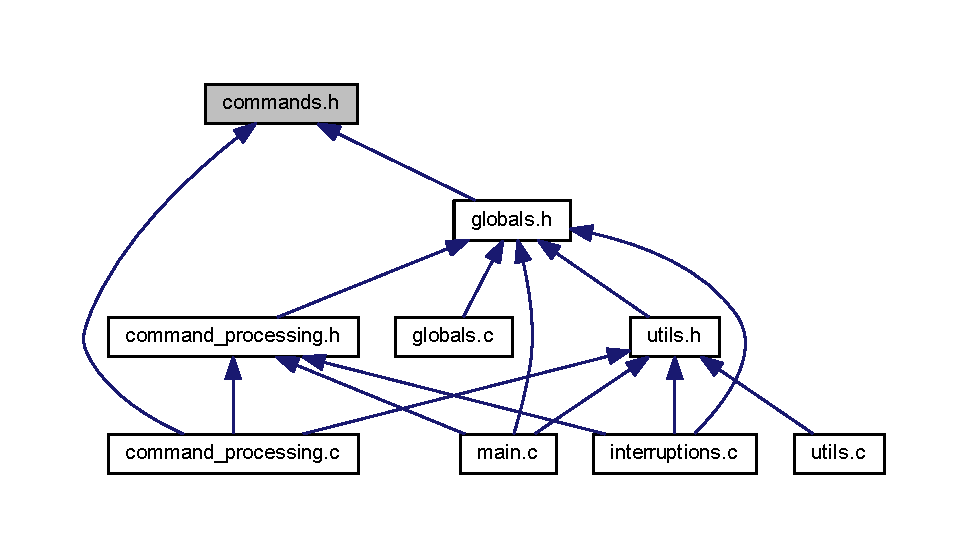
\includegraphics[width=350pt]{commands_8h__dep__incl}
\end{center}
\end{figure}
\doxysubsection*{Macros}
\begin{Indent}\textbf{ QB Move Information Strings}\par
\begin{DoxyCompactItemize}
\item 
\mbox{\label{commands_8h_a2ba44fc5b8a316bd307d0baa9ab629ef}} 
\#define {\bfseries INFO\+\_\+\+ALL}~0
\begin{DoxyCompactList}\small\item\em All system information. \end{DoxyCompactList}\end{DoxyCompactItemize}
\end{Indent}
\doxysubsection*{Enumerations}
\begin{Indent}\textbf{ qb\+Move and qb\+Hand Commands}\par
\begin{DoxyCompactItemize}
\item 
enum \textbf{ qbmove\+\_\+command} \{ \newline
\textbf{ CMD\+\_\+\+PING} = 0
, \textbf{ CMD\+\_\+\+SET\+\_\+\+ZEROS} = 1
, \textbf{ CMD\+\_\+\+STORE\+\_\+\+PARAMS} = 3
, \textbf{ CMD\+\_\+\+STORE\+\_\+\+DEFAULT\+\_\+\+PARAMS} = 4
, \newline
\textbf{ CMD\+\_\+\+RESTORE\+\_\+\+PARAMS} = 5
, \textbf{ CMD\+\_\+\+GET\+\_\+\+INFO} = 6
, \textbf{ CMD\+\_\+\+SET\+\_\+\+VALUE} = 7
, \textbf{ CMD\+\_\+\+GET\+\_\+\+VALUE} = 8
, \newline
\textbf{ CMD\+\_\+\+BOOTLOADER} = 9
, \textbf{ CMD\+\_\+\+INIT\+\_\+\+MEM} = 10
, \textbf{ CMD\+\_\+\+CALIBRATE} = 11
, \textbf{ CMD\+\_\+\+GET\+\_\+\+PARAM\+\_\+\+LIST} = 12
, \newline
\textbf{ CMD\+\_\+\+HAND\+\_\+\+CALIBRATE} = 13
, \textbf{ CMD\+\_\+\+ACTIVATE} = 128
, \textbf{ CMD\+\_\+\+GET\+\_\+\+ACTIVATE} = 129
, \textbf{ CMD\+\_\+\+SET\+\_\+\+INPUTS} = 130
, \newline
\textbf{ CMD\+\_\+\+GET\+\_\+\+INPUTS} = 131
, \textbf{ CMD\+\_\+\+GET\+\_\+\+MEASUREMENTS} = 132
, \textbf{ CMD\+\_\+\+GET\+\_\+\+CURRENTS} = 133
, \textbf{ CMD\+\_\+\+GET\+\_\+\+CURR\+\_\+\+AND\+\_\+\+MEAS} = 134
, \newline
\textbf{ CMD\+\_\+\+SET\+\_\+\+POS\+\_\+\+STIFF} = 135
, \textbf{ CMD\+\_\+\+GET\+\_\+\+EMG} = 136
, \textbf{ CMD\+\_\+\+GET\+\_\+\+VELOCITIES} = 137
, \textbf{ CMD\+\_\+\+GET\+\_\+\+COUNTERS} = 138
, \newline
\textbf{ CMD\+\_\+\+GET\+\_\+\+ACCEL} = 139
, \textbf{ CMD\+\_\+\+GET\+\_\+\+CURR\+\_\+\+DIFF} = 140
, \textbf{ CMD\+\_\+\+SET\+\_\+\+CURR\+\_\+\+DIFF} = 141
, \textbf{ CMD\+\_\+\+SET\+\_\+\+CUFF\+\_\+\+INPUTS} = 142
, \newline
\textbf{ CMD\+\_\+\+SET\+\_\+\+WATCHDOG} = 143
, \textbf{ CMD\+\_\+\+SET\+\_\+\+BAUDRATE} = 144
, \textbf{ CMD\+\_\+\+EXT\+\_\+\+DRIVE} = 145
, \textbf{ CMD\+\_\+\+GET\+\_\+\+JOYSTICK} = 146
 \}
\end{DoxyCompactItemize}
\end{Indent}
\doxysubsection*{qb\+Move and qb\+Hand Parameters}
\begin{DoxyCompactItemize}
\item 
\mbox{\label{commands_8h_ae3302107827a773be3200e459e7b24da}} 
\#define {\bfseries PARAM\+\_\+\+BYTE\+\_\+\+SLOT}~50
\begin{DoxyCompactList}\small\item\em Number of bytes reserved to a param information. \end{DoxyCompactList}\item 
\mbox{\label{commands_8h_a3bab5133f6aa363d84307b39e17b0d74}} 
\#define {\bfseries PARAM\+\_\+\+MENU\+\_\+\+SLOT}~150
\begin{DoxyCompactList}\small\item\em Number of bytes reserved to a param menu. \end{DoxyCompactList}\item 
enum \textbf{ qbmove\+\_\+parameter} \{ \newline
\textbf{ PARAM\+\_\+\+ID} = 0
, \textbf{ PARAM\+\_\+\+PID\+\_\+\+CONTROL} = 1
, \textbf{ PARAM\+\_\+\+STARTUP\+\_\+\+ACTIVATION} = 2
, \textbf{ PARAM\+\_\+\+INPUT\+\_\+\+MODE} = 3
, \newline
\textbf{ PARAM\+\_\+\+CONTROL\+\_\+\+MODE} = 4
, \textbf{ PARAM\+\_\+\+MEASUREMENT\+\_\+\+OFFSET} = 5
, \textbf{ PARAM\+\_\+\+MEASUREMENT\+\_\+\+MULTIPLIER} = 6
, \textbf{ PARAM\+\_\+\+POS\+\_\+\+LIMIT\+\_\+\+FLAG} = 7
, \newline
\textbf{ PARAM\+\_\+\+POS\+\_\+\+LIMIT} = 8
, \textbf{ PARAM\+\_\+\+MAX\+\_\+\+STEP\+\_\+\+POS} = 9
, \textbf{ PARAM\+\_\+\+MAX\+\_\+\+STEP\+\_\+\+NEG} = 10
, \textbf{ PARAM\+\_\+\+POS\+\_\+\+RESOLUTION} = 11
, \newline
\textbf{ PARAM\+\_\+\+CURRENT\+\_\+\+LIMIT} = 12
, \textbf{ PARAM\+\_\+\+EMG\+\_\+\+CALIB\+\_\+\+FLAG} = 13
, \textbf{ PARAM\+\_\+\+EMG\+\_\+\+THRESHOLD} = 14
, \textbf{ PARAM\+\_\+\+EMG\+\_\+\+MAX\+\_\+\+VALUE} = 15
, \newline
\textbf{ PARAM\+\_\+\+EMG\+\_\+\+SPEED} = 16
, \textbf{ PARAM\+\_\+\+PID\+\_\+\+CURR\+\_\+\+CONTROL} = 18
, \textbf{ PARAM\+\_\+\+DOUBLE\+\_\+\+ENC\+\_\+\+ON\+\_\+\+OFF} = 19
, \textbf{ PARAM\+\_\+\+MOT\+\_\+\+HANDLE\+\_\+\+RATIO} = 20
, \newline
\textbf{ PARAM\+\_\+\+MOTOR\+\_\+\+SUPPLY} = 21
, \textbf{ PARAM\+\_\+\+CURRENT\+\_\+\+LOOKUP} = 23
, \textbf{ PARAM\+\_\+\+DL\+\_\+\+POS\+\_\+\+PID} = 24
, \textbf{ PARAM\+\_\+\+DL\+\_\+\+CURR\+\_\+\+PID} = 25
 \}
\item 
\mbox{\label{commands_8h_ad18f2ef316ee226b52882af5758c39e8}} 
enum {\bfseries qbmove\+\_\+resolution} \{ \newline
{\bfseries RESOLUTION\+\_\+360} = 0
, {\bfseries RESOLUTION\+\_\+720} = 1
, {\bfseries RESOLUTION\+\_\+1440} = 2
, {\bfseries RESOLUTION\+\_\+2880} = 3
, \newline
{\bfseries RESOLUTION\+\_\+5760} = 4
, {\bfseries RESOLUTION\+\_\+11520} = 5
, {\bfseries RESOLUTION\+\_\+23040} = 6
, {\bfseries RESOLUTION\+\_\+46080} = 7
, \newline
{\bfseries RESOLUTION\+\_\+92160} = 8
 \}
\item 
enum \textbf{ qbmove\+\_\+input\+\_\+mode} \{ \newline
\textbf{ INPUT\+\_\+\+MODE\+\_\+\+EXTERNAL} = 0
, \textbf{ INPUT\+\_\+\+MODE\+\_\+\+ENCODER3} = 1
, \textbf{ INPUT\+\_\+\+MODE\+\_\+\+EMG\+\_\+\+PROPORTIONAL} = 2
, \textbf{ INPUT\+\_\+\+MODE\+\_\+\+EMG\+\_\+\+INTEGRAL} = 3
, \newline
\textbf{ INPUT\+\_\+\+MODE\+\_\+\+EMG\+\_\+\+FCFS} = 4
, \textbf{ INPUT\+\_\+\+MODE\+\_\+\+EMG\+\_\+\+FCFS\+\_\+\+ADV} = 5
, \textbf{ INPUT\+\_\+\+MODE\+\_\+\+JOYSTICK} = 6
 \}
\item 
\mbox{\label{commands_8h_a0eae1c82d20671c5d0b9b82b10070f1b}} 
enum {\bfseries acknowledgment\+\_\+values} \{ {\bfseries ACK\+\_\+\+ERROR} = 0
, {\bfseries ACK\+\_\+\+OK} = 1
 \}
\item 
\mbox{\label{commands_8h_aee7544e5fa6e2843ecdc3609602e56aa}} 
enum {\bfseries data\+\_\+types} \{ \newline
{\bfseries TYPE\+\_\+\+FLAG} = 0
, {\bfseries TYPE\+\_\+\+INT8} = 1
, {\bfseries TYPE\+\_\+\+UINT8} = 2
, {\bfseries TYPE\+\_\+\+INT16} = 3
, \newline
{\bfseries TYPE\+\_\+\+UINT16} = 4
, {\bfseries TYPE\+\_\+\+INT32} = 5
, {\bfseries TYPE\+\_\+\+UINT32} = 6
, {\bfseries TYPE\+\_\+\+FLOAT} = 7
, \newline
{\bfseries TYPE\+\_\+\+DOUBLE} = 8
 \}
\end{DoxyCompactItemize}


\doxysubsection{Detailed Description}
Definitions for Soft\+Hand commands, parameters and packages. 

\begin{DoxyDate}{Date}
October 01, 2017 
\end{DoxyDate}
\begin{DoxyAuthor}{Author}
{\itshape Centro \char`\"{}\+E.\+Piaggio\char`\"{}} 
\end{DoxyAuthor}
\begin{DoxyCopyright}{Copyright}
(C) 2012-\/2016 qbrobotics. All rights reserved. 

(C) 2017 Centro \char`\"{}\+E.\+Piaggio\char`\"{}. All rights reserved.
\end{DoxyCopyright}
This file is included in the firmware, in its libraries and applications. It contains all definitions that are necessary for the contruction of communication packages.

It includes definitions for all of the device commands, parameters and also the size of answer packages. 

\doxysubsection{Enumeration Type Documentation}
\mbox{\label{commands_8h_abf0494aabdc65d654a54044eddc9210b}} 
\index{commands.h@{commands.h}!qbmove\_command@{qbmove\_command}}
\index{qbmove\_command@{qbmove\_command}!commands.h@{commands.h}}
\doxysubsubsection{qbmove\_command}
{\footnotesize\ttfamily enum \textbf{ qbmove\+\_\+command}}

\begin{DoxyEnumFields}{Enumerator}
\raisebox{\heightof{T}}[0pt][0pt]{\index{CMD\_PING@{CMD\_PING}!commands.h@{commands.h}}\index{commands.h@{commands.h}!CMD\_PING@{CMD\_PING}}}\mbox{\label{commands_8h_abf0494aabdc65d654a54044eddc9210ba1c0aa24c3612e77ea1a5ca1b82388da0}} 
CMD\+\_\+\+PING&Asks for a ping message. \\
\hline

\raisebox{\heightof{T}}[0pt][0pt]{\index{CMD\_SET\_ZEROS@{CMD\_SET\_ZEROS}!commands.h@{commands.h}}\index{commands.h@{commands.h}!CMD\_SET\_ZEROS@{CMD\_SET\_ZEROS}}}\mbox{\label{commands_8h_abf0494aabdc65d654a54044eddc9210ba2d92e89157e03fe63bfebf8125c3a0d7}} 
CMD\+\_\+\+SET\+\_\+\+ZEROS&Command for setting the encoders zero position. \\
\hline

\raisebox{\heightof{T}}[0pt][0pt]{\index{CMD\_STORE\_PARAMS@{CMD\_STORE\_PARAMS}!commands.h@{commands.h}}\index{commands.h@{commands.h}!CMD\_STORE\_PARAMS@{CMD\_STORE\_PARAMS}}}\mbox{\label{commands_8h_abf0494aabdc65d654a54044eddc9210bac7d1170961179d8dc5ec1b4aeb4f3116}} 
CMD\+\_\+\+STORE\+\_\+\+PARAMS&Stores all parameters in memory and loads them. \\
\hline

\raisebox{\heightof{T}}[0pt][0pt]{\index{CMD\_STORE\_DEFAULT\_PARAMS@{CMD\_STORE\_DEFAULT\_PARAMS}!commands.h@{commands.h}}\index{commands.h@{commands.h}!CMD\_STORE\_DEFAULT\_PARAMS@{CMD\_STORE\_DEFAULT\_PARAMS}}}\mbox{\label{commands_8h_abf0494aabdc65d654a54044eddc9210ba17d9c730cd01059737de14b9f062e44c}} 
CMD\+\_\+\+STORE\+\_\+\+DEFAULT\+\_\+\+PARAMS&Store current parameters as factory parameters. \\
\hline

\raisebox{\heightof{T}}[0pt][0pt]{\index{CMD\_RESTORE\_PARAMS@{CMD\_RESTORE\_PARAMS}!commands.h@{commands.h}}\index{commands.h@{commands.h}!CMD\_RESTORE\_PARAMS@{CMD\_RESTORE\_PARAMS}}}\mbox{\label{commands_8h_abf0494aabdc65d654a54044eddc9210ba7f13c143f54c74572776ffae219d33d7}} 
CMD\+\_\+\+RESTORE\+\_\+\+PARAMS&Restore default factory parameters. \\
\hline

\raisebox{\heightof{T}}[0pt][0pt]{\index{CMD\_GET\_INFO@{CMD\_GET\_INFO}!commands.h@{commands.h}}\index{commands.h@{commands.h}!CMD\_GET\_INFO@{CMD\_GET\_INFO}}}\mbox{\label{commands_8h_abf0494aabdc65d654a54044eddc9210ba4681b714888632a2d8ad0a2140e4ba7f}} 
CMD\+\_\+\+GET\+\_\+\+INFO&Asks for a string of information about. \\
\hline

\raisebox{\heightof{T}}[0pt][0pt]{\index{CMD\_SET\_VALUE@{CMD\_SET\_VALUE}!commands.h@{commands.h}}\index{commands.h@{commands.h}!CMD\_SET\_VALUE@{CMD\_SET\_VALUE}}}\mbox{\label{commands_8h_abf0494aabdc65d654a54044eddc9210bac3ca8989b510cb78baff4425a0d47a67}} 
CMD\+\_\+\+SET\+\_\+\+VALUE&Not Used. \\
\hline

\raisebox{\heightof{T}}[0pt][0pt]{\index{CMD\_GET\_VALUE@{CMD\_GET\_VALUE}!commands.h@{commands.h}}\index{commands.h@{commands.h}!CMD\_GET\_VALUE@{CMD\_GET\_VALUE}}}\mbox{\label{commands_8h_abf0494aabdc65d654a54044eddc9210bac9a592ed746a114c7bfc0bd9d094263c}} 
CMD\+\_\+\+GET\+\_\+\+VALUE&Not Used. \\
\hline

\raisebox{\heightof{T}}[0pt][0pt]{\index{CMD\_BOOTLOADER@{CMD\_BOOTLOADER}!commands.h@{commands.h}}\index{commands.h@{commands.h}!CMD\_BOOTLOADER@{CMD\_BOOTLOADER}}}\mbox{\label{commands_8h_abf0494aabdc65d654a54044eddc9210bac72c6075e3464ea5abbe0c0d6e11559e}} 
CMD\+\_\+\+BOOTLOADER&Sets the bootloader modality to update the firmware. \\
\hline

\raisebox{\heightof{T}}[0pt][0pt]{\index{CMD\_INIT\_MEM@{CMD\_INIT\_MEM}!commands.h@{commands.h}}\index{commands.h@{commands.h}!CMD\_INIT\_MEM@{CMD\_INIT\_MEM}}}\mbox{\label{commands_8h_abf0494aabdc65d654a54044eddc9210ba7bd24a7ad88af9a4e7c398a9ecb08ed4}} 
CMD\+\_\+\+INIT\+\_\+\+MEM&Initialize the memory with the defalut values. \\
\hline

\raisebox{\heightof{T}}[0pt][0pt]{\index{CMD\_CALIBRATE@{CMD\_CALIBRATE}!commands.h@{commands.h}}\index{commands.h@{commands.h}!CMD\_CALIBRATE@{CMD\_CALIBRATE}}}\mbox{\label{commands_8h_abf0494aabdc65d654a54044eddc9210ba238830aded332d3bd5cbbb4ea2cb6ce7}} 
CMD\+\_\+\+CALIBRATE&Starts the stiffness calibration of the qb\+Move or the hand closure and opening calibration. \\
\hline

\raisebox{\heightof{T}}[0pt][0pt]{\index{CMD\_GET\_PARAM\_LIST@{CMD\_GET\_PARAM\_LIST}!commands.h@{commands.h}}\index{commands.h@{commands.h}!CMD\_GET\_PARAM\_LIST@{CMD\_GET\_PARAM\_LIST}}}\mbox{\label{commands_8h_abf0494aabdc65d654a54044eddc9210ba3e92a6e4c288be3abb6f3cfadf261e78}} 
CMD\+\_\+\+GET\+\_\+\+PARAM\+\_\+\+LIST&Command to get the parameters list or to set a defined value chosen by the use. \\
\hline

\raisebox{\heightof{T}}[0pt][0pt]{\index{CMD\_HAND\_CALIBRATE@{CMD\_HAND\_CALIBRATE}!commands.h@{commands.h}}\index{commands.h@{commands.h}!CMD\_HAND\_CALIBRATE@{CMD\_HAND\_CALIBRATE}}}\mbox{\label{commands_8h_abf0494aabdc65d654a54044eddc9210ba76be5a50e0ac4a9f944d0d6382f06e92}} 
CMD\+\_\+\+HAND\+\_\+\+CALIBRATE&Starts a series of opening and closures of the hand. \\
\hline

\raisebox{\heightof{T}}[0pt][0pt]{\index{CMD\_ACTIVATE@{CMD\_ACTIVATE}!commands.h@{commands.h}}\index{commands.h@{commands.h}!CMD\_ACTIVATE@{CMD\_ACTIVATE}}}\mbox{\label{commands_8h_abf0494aabdc65d654a54044eddc9210ba341cc0e29a584b4c75a7502529920a7f}} 
CMD\+\_\+\+ACTIVATE&Command for activating/deactivating the device. \\
\hline

\raisebox{\heightof{T}}[0pt][0pt]{\index{CMD\_GET\_ACTIVATE@{CMD\_GET\_ACTIVATE}!commands.h@{commands.h}}\index{commands.h@{commands.h}!CMD\_GET\_ACTIVATE@{CMD\_GET\_ACTIVATE}}}\mbox{\label{commands_8h_abf0494aabdc65d654a54044eddc9210bac56c7ee3592b79204a8f209460ca6531}} 
CMD\+\_\+\+GET\+\_\+\+ACTIVATE&Command for getting device activation state. \\
\hline

\raisebox{\heightof{T}}[0pt][0pt]{\index{CMD\_SET\_INPUTS@{CMD\_SET\_INPUTS}!commands.h@{commands.h}}\index{commands.h@{commands.h}!CMD\_SET\_INPUTS@{CMD\_SET\_INPUTS}}}\mbox{\label{commands_8h_abf0494aabdc65d654a54044eddc9210bac271d0c424b55b263c47f451b3685d65}} 
CMD\+\_\+\+SET\+\_\+\+INPUTS&Command for setting reference inputs. \\
\hline

\raisebox{\heightof{T}}[0pt][0pt]{\index{CMD\_GET\_INPUTS@{CMD\_GET\_INPUTS}!commands.h@{commands.h}}\index{commands.h@{commands.h}!CMD\_GET\_INPUTS@{CMD\_GET\_INPUTS}}}\mbox{\label{commands_8h_abf0494aabdc65d654a54044eddc9210ba7e1020474f9835468c3cfbcce610f7df}} 
CMD\+\_\+\+GET\+\_\+\+INPUTS&Command for getting reference inputs. \\
\hline

\raisebox{\heightof{T}}[0pt][0pt]{\index{CMD\_GET\_MEASUREMENTS@{CMD\_GET\_MEASUREMENTS}!commands.h@{commands.h}}\index{commands.h@{commands.h}!CMD\_GET\_MEASUREMENTS@{CMD\_GET\_MEASUREMENTS}}}\mbox{\label{commands_8h_abf0494aabdc65d654a54044eddc9210bae71f36974018d7c926d1023127ba5018}} 
CMD\+\_\+\+GET\+\_\+\+MEASUREMENTS&Command for asking device\textquotesingle{}s position measurements. \\
\hline

\raisebox{\heightof{T}}[0pt][0pt]{\index{CMD\_GET\_CURRENTS@{CMD\_GET\_CURRENTS}!commands.h@{commands.h}}\index{commands.h@{commands.h}!CMD\_GET\_CURRENTS@{CMD\_GET\_CURRENTS}}}\mbox{\label{commands_8h_abf0494aabdc65d654a54044eddc9210ba7cec1501d2f9057540987c1f9f3eaf2d}} 
CMD\+\_\+\+GET\+\_\+\+CURRENTS&Command for asking device\textquotesingle{}s current measurements. \\
\hline

\raisebox{\heightof{T}}[0pt][0pt]{\index{CMD\_GET\_CURR\_AND\_MEAS@{CMD\_GET\_CURR\_AND\_MEAS}!commands.h@{commands.h}}\index{commands.h@{commands.h}!CMD\_GET\_CURR\_AND\_MEAS@{CMD\_GET\_CURR\_AND\_MEAS}}}\mbox{\label{commands_8h_abf0494aabdc65d654a54044eddc9210ba00e1e21809cce47849f8d237b14c9e17}} 
CMD\+\_\+\+GET\+\_\+\+CURR\+\_\+\+AND\+\_\+\+MEAS&Command for asking device\textquotesingle{}s measurements and currents. \\
\hline

\raisebox{\heightof{T}}[0pt][0pt]{\index{CMD\_SET\_POS\_STIFF@{CMD\_SET\_POS\_STIFF}!commands.h@{commands.h}}\index{commands.h@{commands.h}!CMD\_SET\_POS\_STIFF@{CMD\_SET\_POS\_STIFF}}}\mbox{\label{commands_8h_abf0494aabdc65d654a54044eddc9210baa8ff629570855ac5162560c19fcbd374}} 
CMD\+\_\+\+SET\+\_\+\+POS\+\_\+\+STIFF&Not used in the softhand firmware. \\
\hline

\raisebox{\heightof{T}}[0pt][0pt]{\index{CMD\_GET\_EMG@{CMD\_GET\_EMG}!commands.h@{commands.h}}\index{commands.h@{commands.h}!CMD\_GET\_EMG@{CMD\_GET\_EMG}}}\mbox{\label{commands_8h_abf0494aabdc65d654a54044eddc9210baf64fae1b253023ea4d6307619fb00bd6}} 
CMD\+\_\+\+GET\+\_\+\+EMG&Command for asking device\textquotesingle{}s emg sensors measurements. \\
\hline

\raisebox{\heightof{T}}[0pt][0pt]{\index{CMD\_GET\_VELOCITIES@{CMD\_GET\_VELOCITIES}!commands.h@{commands.h}}\index{commands.h@{commands.h}!CMD\_GET\_VELOCITIES@{CMD\_GET\_VELOCITIES}}}\mbox{\label{commands_8h_abf0494aabdc65d654a54044eddc9210ba91f95871982459406bcbfa9e84affcf8}} 
CMD\+\_\+\+GET\+\_\+\+VELOCITIES&Command for asking device\textquotesingle{}s velocity measurements. \\
\hline

\raisebox{\heightof{T}}[0pt][0pt]{\index{CMD\_GET\_COUNTERS@{CMD\_GET\_COUNTERS}!commands.h@{commands.h}}\index{commands.h@{commands.h}!CMD\_GET\_COUNTERS@{CMD\_GET\_COUNTERS}}}\mbox{\label{commands_8h_abf0494aabdc65d654a54044eddc9210ba852a1e9b4cec526ef7b4e550cee73cae}} 
CMD\+\_\+\+GET\+\_\+\+COUNTERS&Command for asking device\textquotesingle{}s counters (mostly used for debugging sent commands). \\
\hline

\raisebox{\heightof{T}}[0pt][0pt]{\index{CMD\_GET\_ACCEL@{CMD\_GET\_ACCEL}!commands.h@{commands.h}}\index{commands.h@{commands.h}!CMD\_GET\_ACCEL@{CMD\_GET\_ACCEL}}}\mbox{\label{commands_8h_abf0494aabdc65d654a54044eddc9210ba62e954ab85dca16967b1d2b11f099515}} 
CMD\+\_\+\+GET\+\_\+\+ACCEL&Command for asking device\textquotesingle{}s acceleration measurements. \\
\hline

\raisebox{\heightof{T}}[0pt][0pt]{\index{CMD\_GET\_CURR\_DIFF@{CMD\_GET\_CURR\_DIFF}!commands.h@{commands.h}}\index{commands.h@{commands.h}!CMD\_GET\_CURR\_DIFF@{CMD\_GET\_CURR\_DIFF}}}\mbox{\label{commands_8h_abf0494aabdc65d654a54044eddc9210bac1a1e6554eb0603ea5a5f77f604f594c}} 
CMD\+\_\+\+GET\+\_\+\+CURR\+\_\+\+DIFF&Command for asking device\textquotesingle{}s current difference between a measured one and an estimated one (Only for Soft\+Hand). \\
\hline

\raisebox{\heightof{T}}[0pt][0pt]{\index{CMD\_SET\_CURR\_DIFF@{CMD\_SET\_CURR\_DIFF}!commands.h@{commands.h}}\index{commands.h@{commands.h}!CMD\_SET\_CURR\_DIFF@{CMD\_SET\_CURR\_DIFF}}}\mbox{\label{commands_8h_abf0494aabdc65d654a54044eddc9210ba75bb0f4bbebcfa9d066c0d1f41531127}} 
CMD\+\_\+\+SET\+\_\+\+CURR\+\_\+\+DIFF&Command used to set current difference modality (Only for Cuff device). \\
\hline

\raisebox{\heightof{T}}[0pt][0pt]{\index{CMD\_SET\_CUFF\_INPUTS@{CMD\_SET\_CUFF\_INPUTS}!commands.h@{commands.h}}\index{commands.h@{commands.h}!CMD\_SET\_CUFF\_INPUTS@{CMD\_SET\_CUFF\_INPUTS}}}\mbox{\label{commands_8h_abf0494aabdc65d654a54044eddc9210ba78d9d45e499f848da1c4d03a1ba534a4}} 
CMD\+\_\+\+SET\+\_\+\+CUFF\+\_\+\+INPUTS&Command used to set Cuff device inputs (Only for Cuff device). \\
\hline

\raisebox{\heightof{T}}[0pt][0pt]{\index{CMD\_SET\_WATCHDOG@{CMD\_SET\_WATCHDOG}!commands.h@{commands.h}}\index{commands.h@{commands.h}!CMD\_SET\_WATCHDOG@{CMD\_SET\_WATCHDOG}}}\mbox{\label{commands_8h_abf0494aabdc65d654a54044eddc9210ba4fa373fa933adfa01f2a9bea1281aa2f}} 
CMD\+\_\+\+SET\+\_\+\+WATCHDOG&Command for setting watchdog timer or disable it. \\
\hline

\raisebox{\heightof{T}}[0pt][0pt]{\index{CMD\_SET\_BAUDRATE@{CMD\_SET\_BAUDRATE}!commands.h@{commands.h}}\index{commands.h@{commands.h}!CMD\_SET\_BAUDRATE@{CMD\_SET\_BAUDRATE}}}\mbox{\label{commands_8h_abf0494aabdc65d654a54044eddc9210ba2ddc0e8c5f0a28ad470e881d1e196c47}} 
CMD\+\_\+\+SET\+\_\+\+BAUDRATE&Command for setting baudrate of communication. \\
\hline

\raisebox{\heightof{T}}[0pt][0pt]{\index{CMD\_EXT\_DRIVE@{CMD\_EXT\_DRIVE}!commands.h@{commands.h}}\index{commands.h@{commands.h}!CMD\_EXT\_DRIVE@{CMD\_EXT\_DRIVE}}}\mbox{\label{commands_8h_abf0494aabdc65d654a54044eddc9210ba533b9dc5738b9a717fff08f29278b8a5}} 
CMD\+\_\+\+EXT\+\_\+\+DRIVE&Command to set the actual measurements as inputs to another device (Only for Armslider device). \\
\hline

\raisebox{\heightof{T}}[0pt][0pt]{\index{CMD\_GET\_JOYSTICK@{CMD\_GET\_JOYSTICK}!commands.h@{commands.h}}\index{commands.h@{commands.h}!CMD\_GET\_JOYSTICK@{CMD\_GET\_JOYSTICK}}}\mbox{\label{commands_8h_abf0494aabdc65d654a54044eddc9210ba51f92ae4cb4dffafda985f714433039a}} 
CMD\+\_\+\+GET\+\_\+\+JOYSTICK&Command to get the joystick measurements (Only ~\newline
 \\
\hline

\end{DoxyEnumFields}
\mbox{\label{commands_8h_a4c6f8687cc4a70ce967c910614fbc6cd}} 
\index{commands.h@{commands.h}!qbmove\_input\_mode@{qbmove\_input\_mode}}
\index{qbmove\_input\_mode@{qbmove\_input\_mode}!commands.h@{commands.h}}
\doxysubsubsection{qbmove\_input\_mode}
{\footnotesize\ttfamily enum \textbf{ qbmove\+\_\+input\+\_\+mode}}

\begin{DoxyEnumFields}{Enumerator}
\raisebox{\heightof{T}}[0pt][0pt]{\index{INPUT\_MODE\_EXTERNAL@{INPUT\_MODE\_EXTERNAL}!commands.h@{commands.h}}\index{commands.h@{commands.h}!INPUT\_MODE\_EXTERNAL@{INPUT\_MODE\_EXTERNAL}}}\mbox{\label{commands_8h_a4c6f8687cc4a70ce967c910614fbc6cdae9164f9cc9192eb336b04d078f46b8ba}} 
INPUT\+\_\+\+MODE\+\_\+\+EXTERNAL&References through external commands (default). \\
\hline

\raisebox{\heightof{T}}[0pt][0pt]{\index{INPUT\_MODE\_ENCODER3@{INPUT\_MODE\_ENCODER3}!commands.h@{commands.h}}\index{commands.h@{commands.h}!INPUT\_MODE\_ENCODER3@{INPUT\_MODE\_ENCODER3}}}\mbox{\label{commands_8h_a4c6f8687cc4a70ce967c910614fbc6cda9bfa7271b88d5876a1c3fd050f67bd3e}} 
INPUT\+\_\+\+MODE\+\_\+\+ENCODER3&Encoder 3 drives all inputs. \\
\hline

\raisebox{\heightof{T}}[0pt][0pt]{\index{INPUT\_MODE\_EMG\_PROPORTIONAL@{INPUT\_MODE\_EMG\_PROPORTIONAL}!commands.h@{commands.h}}\index{commands.h@{commands.h}!INPUT\_MODE\_EMG\_PROPORTIONAL@{INPUT\_MODE\_EMG\_PROPORTIONAL}}}\mbox{\label{commands_8h_a4c6f8687cc4a70ce967c910614fbc6cda791c735316bd375c6e93d561cb80eafd}} 
INPUT\+\_\+\+MODE\+\_\+\+EMG\+\_\+\+PROPORTIONAL&Use EMG measure to proportionally drive the position of the motor 1. \\
\hline

\raisebox{\heightof{T}}[0pt][0pt]{\index{INPUT\_MODE\_EMG\_INTEGRAL@{INPUT\_MODE\_EMG\_INTEGRAL}!commands.h@{commands.h}}\index{commands.h@{commands.h}!INPUT\_MODE\_EMG\_INTEGRAL@{INPUT\_MODE\_EMG\_INTEGRAL}}}\mbox{\label{commands_8h_a4c6f8687cc4a70ce967c910614fbc6cda9ccbbc4cd825d977b0b089b9121cfac5}} 
INPUT\+\_\+\+MODE\+\_\+\+EMG\+\_\+\+INTEGRAL&Use 2 EMG signals to drive motor position. \\
\hline

\raisebox{\heightof{T}}[0pt][0pt]{\index{INPUT\_MODE\_EMG\_FCFS@{INPUT\_MODE\_EMG\_FCFS}!commands.h@{commands.h}}\index{commands.h@{commands.h}!INPUT\_MODE\_EMG\_FCFS@{INPUT\_MODE\_EMG\_FCFS}}}\mbox{\label{commands_8h_a4c6f8687cc4a70ce967c910614fbc6cda63042e0fb1fcf5bf0008b15442eea194}} 
INPUT\+\_\+\+MODE\+\_\+\+EMG\+\_\+\+FCFS&Use 2 EMG. First reaching threshold wins and its value defines hand closure. \\
\hline

\raisebox{\heightof{T}}[0pt][0pt]{\index{INPUT\_MODE\_EMG\_FCFS\_ADV@{INPUT\_MODE\_EMG\_FCFS\_ADV}!commands.h@{commands.h}}\index{commands.h@{commands.h}!INPUT\_MODE\_EMG\_FCFS\_ADV@{INPUT\_MODE\_EMG\_FCFS\_ADV}}}\mbox{\label{commands_8h_a4c6f8687cc4a70ce967c910614fbc6cda9e54aef6ab6f164ed0db5c3d59058da8}} 
INPUT\+\_\+\+MODE\+\_\+\+EMG\+\_\+\+FCFS\+\_\+\+ADV&Use 2 EMG. First reaching threshold wins and its value defines hand closure Wait for both EMG to lower under threshold. \\
\hline

\raisebox{\heightof{T}}[0pt][0pt]{\index{INPUT\_MODE\_JOYSTICK@{INPUT\_MODE\_JOYSTICK}!commands.h@{commands.h}}\index{commands.h@{commands.h}!INPUT\_MODE\_JOYSTICK@{INPUT\_MODE\_JOYSTICK}}}\mbox{\label{commands_8h_a4c6f8687cc4a70ce967c910614fbc6cda6f5918e455c85bc7e916bddbf8889538}} 
INPUT\+\_\+\+MODE\+\_\+\+JOYSTICK&Joystick input mode. \\
\hline

\end{DoxyEnumFields}
\mbox{\label{commands_8h_a0f1ee428e49fc602d6fde71d7ff80f36}} 
\index{commands.h@{commands.h}!qbmove\_parameter@{qbmove\_parameter}}
\index{qbmove\_parameter@{qbmove\_parameter}!commands.h@{commands.h}}
\doxysubsubsection{qbmove\_parameter}
{\footnotesize\ttfamily enum \textbf{ qbmove\+\_\+parameter}}

\begin{DoxyEnumFields}{Enumerator}
\raisebox{\heightof{T}}[0pt][0pt]{\index{PARAM\_ID@{PARAM\_ID}!commands.h@{commands.h}}\index{commands.h@{commands.h}!PARAM\_ID@{PARAM\_ID}}}\mbox{\label{commands_8h_a0f1ee428e49fc602d6fde71d7ff80f36a172b8d344a5aaae4d87daa52e36e9e5f}} 
PARAM\+\_\+\+ID&Device\textquotesingle{}s ID number. \\
\hline

\raisebox{\heightof{T}}[0pt][0pt]{\index{PARAM\_PID\_CONTROL@{PARAM\_PID\_CONTROL}!commands.h@{commands.h}}\index{commands.h@{commands.h}!PARAM\_PID\_CONTROL@{PARAM\_PID\_CONTROL}}}\mbox{\label{commands_8h_a0f1ee428e49fc602d6fde71d7ff80f36a878e85d61c0bca0141e6118d1ceba299}} 
PARAM\+\_\+\+PID\+\_\+\+CONTROL&PID parameters. \\
\hline

\raisebox{\heightof{T}}[0pt][0pt]{\index{PARAM\_STARTUP\_ACTIVATION@{PARAM\_STARTUP\_ACTIVATION}!commands.h@{commands.h}}\index{commands.h@{commands.h}!PARAM\_STARTUP\_ACTIVATION@{PARAM\_STARTUP\_ACTIVATION}}}\mbox{\label{commands_8h_a0f1ee428e49fc602d6fde71d7ff80f36a9f7e2f9c7b92726e1ffd5dda3af47fd8}} 
PARAM\+\_\+\+STARTUP\+\_\+\+ACTIVATION&Start up activation byte. \\
\hline

\raisebox{\heightof{T}}[0pt][0pt]{\index{PARAM\_INPUT\_MODE@{PARAM\_INPUT\_MODE}!commands.h@{commands.h}}\index{commands.h@{commands.h}!PARAM\_INPUT\_MODE@{PARAM\_INPUT\_MODE}}}\mbox{\label{commands_8h_a0f1ee428e49fc602d6fde71d7ff80f36a5c697f31b90e98e2eba960b79f2ed25c}} 
PARAM\+\_\+\+INPUT\+\_\+\+MODE&Input mode. \\
\hline

\raisebox{\heightof{T}}[0pt][0pt]{\index{PARAM\_CONTROL\_MODE@{PARAM\_CONTROL\_MODE}!commands.h@{commands.h}}\index{commands.h@{commands.h}!PARAM\_CONTROL\_MODE@{PARAM\_CONTROL\_MODE}}}\mbox{\label{commands_8h_a0f1ee428e49fc602d6fde71d7ff80f36aad84d584a61a3575db214d10d9bb6cb0}} 
PARAM\+\_\+\+CONTROL\+\_\+\+MODE&Choose the kind of control between position control, current control, direct PWM value or current+position control. \\
\hline

\raisebox{\heightof{T}}[0pt][0pt]{\index{PARAM\_MEASUREMENT\_OFFSET@{PARAM\_MEASUREMENT\_OFFSET}!commands.h@{commands.h}}\index{commands.h@{commands.h}!PARAM\_MEASUREMENT\_OFFSET@{PARAM\_MEASUREMENT\_OFFSET}}}\mbox{\label{commands_8h_a0f1ee428e49fc602d6fde71d7ff80f36adcdce0ed2b6b62335e8986a1758819d5}} 
PARAM\+\_\+\+MEASUREMENT\+\_\+\+OFFSET&Adds a constant offset to the measurements. \\
\hline

\raisebox{\heightof{T}}[0pt][0pt]{\index{PARAM\_MEASUREMENT\_MULTIPLIER@{PARAM\_MEASUREMENT\_MULTIPLIER}!commands.h@{commands.h}}\index{commands.h@{commands.h}!PARAM\_MEASUREMENT\_MULTIPLIER@{PARAM\_MEASUREMENT\_MULTIPLIER}}}\mbox{\label{commands_8h_a0f1ee428e49fc602d6fde71d7ff80f36a547d8f3a487a08ba25a87e5a1c4035a3}} 
PARAM\+\_\+\+MEASUREMENT\+\_\+\+MULTIPLIER&Adds a multiplier to the measurements. \\
\hline

\raisebox{\heightof{T}}[0pt][0pt]{\index{PARAM\_POS\_LIMIT\_FLAG@{PARAM\_POS\_LIMIT\_FLAG}!commands.h@{commands.h}}\index{commands.h@{commands.h}!PARAM\_POS\_LIMIT\_FLAG@{PARAM\_POS\_LIMIT\_FLAG}}}\mbox{\label{commands_8h_a0f1ee428e49fc602d6fde71d7ff80f36ae1ba46d5587fe44580417535c0ccf4fc}} 
PARAM\+\_\+\+POS\+\_\+\+LIMIT\+\_\+\+FLAG&Enable/disable position limiting. \\
\hline

\raisebox{\heightof{T}}[0pt][0pt]{\index{PARAM\_POS\_LIMIT@{PARAM\_POS\_LIMIT}!commands.h@{commands.h}}\index{commands.h@{commands.h}!PARAM\_POS\_LIMIT@{PARAM\_POS\_LIMIT}}}\mbox{\label{commands_8h_a0f1ee428e49fc602d6fde71d7ff80f36a02e68c657a942155b8bd2b037b755011}} 
PARAM\+\_\+\+POS\+\_\+\+LIMIT&Position limit values $\vert$ int32 $\vert$ int32 $\vert$ int32 $\vert$ int32 $\vert$ $\vert$ INF\+\_\+\+LIM\+\_\+1 $\vert$ SUP\+\_\+\+LIM\+\_\+1 $\vert$ INF\+\_\+\+LIM\+\_\+2 $\vert$ SUP\+\_\+\+LIM\+\_\+2 $\vert$ \\
\hline

\raisebox{\heightof{T}}[0pt][0pt]{\index{PARAM\_MAX\_STEP\_POS@{PARAM\_MAX\_STEP\_POS}!commands.h@{commands.h}}\index{commands.h@{commands.h}!PARAM\_MAX\_STEP\_POS@{PARAM\_MAX\_STEP\_POS}}}\mbox{\label{commands_8h_a0f1ee428e49fc602d6fde71d7ff80f36a9e5ffa64ed5e03da3fa0cc5f1b1cd2ae}} 
PARAM\+\_\+\+MAX\+\_\+\+STEP\+\_\+\+POS&Used to slow down movements for positive values. \\
\hline

\raisebox{\heightof{T}}[0pt][0pt]{\index{PARAM\_MAX\_STEP\_NEG@{PARAM\_MAX\_STEP\_NEG}!commands.h@{commands.h}}\index{commands.h@{commands.h}!PARAM\_MAX\_STEP\_NEG@{PARAM\_MAX\_STEP\_NEG}}}\mbox{\label{commands_8h_a0f1ee428e49fc602d6fde71d7ff80f36a5f7c88ebecbc39113c0621701cfedd07}} 
PARAM\+\_\+\+MAX\+\_\+\+STEP\+\_\+\+NEG&Used to slow down movements for negative values. \\
\hline

\raisebox{\heightof{T}}[0pt][0pt]{\index{PARAM\_POS\_RESOLUTION@{PARAM\_POS\_RESOLUTION}!commands.h@{commands.h}}\index{commands.h@{commands.h}!PARAM\_POS\_RESOLUTION@{PARAM\_POS\_RESOLUTION}}}\mbox{\label{commands_8h_a0f1ee428e49fc602d6fde71d7ff80f36a6857aadbe11091d0d3cebe2c22da1eba}} 
PARAM\+\_\+\+POS\+\_\+\+RESOLUTION&Angle resolution for inputs and measurements. Used during communication. \\
\hline

\raisebox{\heightof{T}}[0pt][0pt]{\index{PARAM\_CURRENT\_LIMIT@{PARAM\_CURRENT\_LIMIT}!commands.h@{commands.h}}\index{commands.h@{commands.h}!PARAM\_CURRENT\_LIMIT@{PARAM\_CURRENT\_LIMIT}}}\mbox{\label{commands_8h_a0f1ee428e49fc602d6fde71d7ff80f36a079999b78cd63f61764700fad99990de}} 
PARAM\+\_\+\+CURRENT\+\_\+\+LIMIT&Limit for absorbed current. \\
\hline

\raisebox{\heightof{T}}[0pt][0pt]{\index{PARAM\_EMG\_CALIB\_FLAG@{PARAM\_EMG\_CALIB\_FLAG}!commands.h@{commands.h}}\index{commands.h@{commands.h}!PARAM\_EMG\_CALIB\_FLAG@{PARAM\_EMG\_CALIB\_FLAG}}}\mbox{\label{commands_8h_a0f1ee428e49fc602d6fde71d7ff80f36ae4c6b7c830d9065cee4039a489274b2f}} 
PARAM\+\_\+\+EMG\+\_\+\+CALIB\+\_\+\+FLAG&Enable calibration on startup. \\
\hline

\raisebox{\heightof{T}}[0pt][0pt]{\index{PARAM\_EMG\_THRESHOLD@{PARAM\_EMG\_THRESHOLD}!commands.h@{commands.h}}\index{commands.h@{commands.h}!PARAM\_EMG\_THRESHOLD@{PARAM\_EMG\_THRESHOLD}}}\mbox{\label{commands_8h_a0f1ee428e49fc602d6fde71d7ff80f36aa1d42c709c9c12afffae0921126d9cbf}} 
PARAM\+\_\+\+EMG\+\_\+\+THRESHOLD&Minimum value to have effect. \\
\hline

\raisebox{\heightof{T}}[0pt][0pt]{\index{PARAM\_EMG\_MAX\_VALUE@{PARAM\_EMG\_MAX\_VALUE}!commands.h@{commands.h}}\index{commands.h@{commands.h}!PARAM\_EMG\_MAX\_VALUE@{PARAM\_EMG\_MAX\_VALUE}}}\mbox{\label{commands_8h_a0f1ee428e49fc602d6fde71d7ff80f36a0cd67acda69d33841a94f55b33d14863}} 
PARAM\+\_\+\+EMG\+\_\+\+MAX\+\_\+\+VALUE&Maximum value of EMG. \\
\hline

\raisebox{\heightof{T}}[0pt][0pt]{\index{PARAM\_EMG\_SPEED@{PARAM\_EMG\_SPEED}!commands.h@{commands.h}}\index{commands.h@{commands.h}!PARAM\_EMG\_SPEED@{PARAM\_EMG\_SPEED}}}\mbox{\label{commands_8h_a0f1ee428e49fc602d6fde71d7ff80f36a028d803ac1aa5cc81d9902f8f519d51d}} 
PARAM\+\_\+\+EMG\+\_\+\+SPEED&Closure speed when using EMG. \\
\hline

\raisebox{\heightof{T}}[0pt][0pt]{\index{PARAM\_PID\_CURR\_CONTROL@{PARAM\_PID\_CURR\_CONTROL}!commands.h@{commands.h}}\index{commands.h@{commands.h}!PARAM\_PID\_CURR\_CONTROL@{PARAM\_PID\_CURR\_CONTROL}}}\mbox{\label{commands_8h_a0f1ee428e49fc602d6fde71d7ff80f36afd84a8c2eb30f2984412ddaddd66ac7f}} 
PARAM\+\_\+\+PID\+\_\+\+CURR\+\_\+\+CONTROL&PID current control. \\
\hline

\raisebox{\heightof{T}}[0pt][0pt]{\index{PARAM\_DOUBLE\_ENC\_ON\_OFF@{PARAM\_DOUBLE\_ENC\_ON\_OFF}!commands.h@{commands.h}}\index{commands.h@{commands.h}!PARAM\_DOUBLE\_ENC\_ON\_OFF@{PARAM\_DOUBLE\_ENC\_ON\_OFF}}}\mbox{\label{commands_8h_a0f1ee428e49fc602d6fde71d7ff80f36a065de456f525cedd222737c24ec7300c}} 
PARAM\+\_\+\+DOUBLE\+\_\+\+ENC\+\_\+\+ON\+\_\+\+OFF&Double Encoder Y/N. \\
\hline

\raisebox{\heightof{T}}[0pt][0pt]{\index{PARAM\_MOT\_HANDLE\_RATIO@{PARAM\_MOT\_HANDLE\_RATIO}!commands.h@{commands.h}}\index{commands.h@{commands.h}!PARAM\_MOT\_HANDLE\_RATIO@{PARAM\_MOT\_HANDLE\_RATIO}}}\mbox{\label{commands_8h_a0f1ee428e49fc602d6fde71d7ff80f36a093ab311eb78fffe19b38dc3e18cd3f8}} 
PARAM\+\_\+\+MOT\+\_\+\+HANDLE\+\_\+\+RATIO&Multiplier between handle and motor. \\
\hline

\raisebox{\heightof{T}}[0pt][0pt]{\index{PARAM\_MOTOR\_SUPPLY@{PARAM\_MOTOR\_SUPPLY}!commands.h@{commands.h}}\index{commands.h@{commands.h}!PARAM\_MOTOR\_SUPPLY@{PARAM\_MOTOR\_SUPPLY}}}\mbox{\label{commands_8h_a0f1ee428e49fc602d6fde71d7ff80f36a9fdaad76676bea4caf32e4e7a1343451}} 
PARAM\+\_\+\+MOTOR\+\_\+\+SUPPLY&Motor supply voltage of the hand. \\
\hline

\raisebox{\heightof{T}}[0pt][0pt]{\index{PARAM\_CURRENT\_LOOKUP@{PARAM\_CURRENT\_LOOKUP}!commands.h@{commands.h}}\index{commands.h@{commands.h}!PARAM\_CURRENT\_LOOKUP@{PARAM\_CURRENT\_LOOKUP}}}\mbox{\label{commands_8h_a0f1ee428e49fc602d6fde71d7ff80f36a29262771f7a72b834aba013747202451}} 
PARAM\+\_\+\+CURRENT\+\_\+\+LOOKUP&Table of values used to calculate an estimated current of the Soft\+Hand. \\
\hline

\raisebox{\heightof{T}}[0pt][0pt]{\index{PARAM\_DL\_POS\_PID@{PARAM\_DL\_POS\_PID}!commands.h@{commands.h}}\index{commands.h@{commands.h}!PARAM\_DL\_POS\_PID@{PARAM\_DL\_POS\_PID}}}\mbox{\label{commands_8h_a0f1ee428e49fc602d6fde71d7ff80f36aed3fbd67f27a50599904c4796f3aee63}} 
PARAM\+\_\+\+DL\+\_\+\+POS\+\_\+\+PID&Double loop position PID. \\
\hline

\raisebox{\heightof{T}}[0pt][0pt]{\index{PARAM\_DL\_CURR\_PID@{PARAM\_DL\_CURR\_PID}!commands.h@{commands.h}}\index{commands.h@{commands.h}!PARAM\_DL\_CURR\_PID@{PARAM\_DL\_CURR\_PID}}}\mbox{\label{commands_8h_a0f1ee428e49fc602d6fde71d7ff80f36ae5c58909acc7d5d6afd5a20fb7bc9620}} 
PARAM\+\_\+\+DL\+\_\+\+CURR\+\_\+\+PID&Double loop current PID. \\
\hline

\end{DoxyEnumFields}

\section{globals.\+c File Reference}
\label{globals_8c}\index{globals.\+c@{globals.\+c}}


Global variables.  


{\ttfamily \#include $<$globals.\+h$>$}\newline
Include dependency graph for globals.\+c\+:
\nopagebreak
\begin{figure}[H]
\begin{center}
\leavevmode
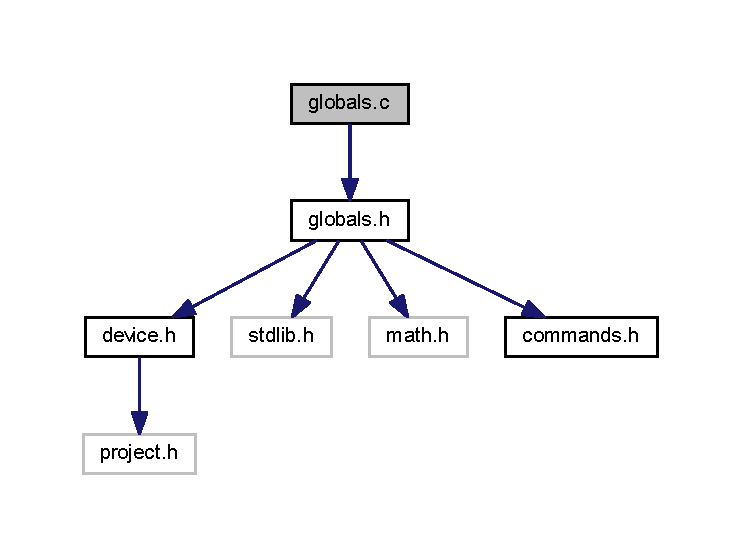
\includegraphics[width=350pt]{globals_8c__incl}
\end{center}
\end{figure}
\subsection*{Variables}
\begin{DoxyCompactItemize}
\item 
struct \textbf{ st\+\_\+ref} g\+\_\+ref g\+\_\+ref\+New \textbf{ g\+\_\+ref\+Old}
\item 
struct \textbf{ st\+\_\+meas} g\+\_\+meas \textbf{ g\+\_\+meas\+Old}
\item 
struct \textbf{ st\+\_\+data} \textbf{ g\+\_\+rx}
\item 
struct \textbf{ st\+\_\+mem} g\+\_\+mem \textbf{ c\+\_\+mem}
\item 
\mbox{\label{globals_8c_aed96fdd8308fe2c4fc07c3b5db1c7bbb}} 
struct \textbf{ st\+\_\+calib} {\bfseries calib}
\item 
float \textbf{ tau\+\_\+feedback}
\item 
uint32 \textbf{ timer\+\_\+value}
\item 
uint32 \textbf{ timer\+\_\+value0}
\item 
int32 \textbf{ dev\+\_\+tension}
\item 
uint8 \textbf{ dev\+\_\+pwm\+\_\+limit}
\item 
int32 \textbf{ dev\+\_\+tension\+\_\+f}
\item 
int32 \textbf{ pow\+\_\+tension}
\item 
C\+Y\+B\+IT \textbf{ reset\+\_\+last\+\_\+value\+\_\+flag}
\item 
C\+Y\+B\+IT \textbf{ tension\+\_\+valid}
\item 
C\+Y\+B\+IT \textbf{ interrupt\+\_\+flag} = F\+A\+L\+SE
\item 
C\+Y\+B\+IT \textbf{ watchdog\+\_\+flag}
\item 
\mbox{\label{globals_8c_abb22f0a4462a0b4db27496654f2175a0}} 
int16 {\bfseries A\+D\+C\+\_\+buf} [4]
\item 
int8 \textbf{ pwm\+\_\+sign}
\item 
uint8 \textbf{ master\+\_\+mode}
\item 
uint8 \textbf{ rest\+\_\+enabled}
\item 
uint8 \textbf{ forced\+\_\+open}
\item 
int32 \textbf{ rest\+\_\+pos\+\_\+curr\+\_\+ref}
\item 
uint8 \textbf{ receive\+\_\+meas\+\_\+from\+\_\+hand}
\item 
\mbox{\label{globals_8c_ab43d57397f71cb35c19d91058c48bed2}} 
int16 {\bfseries check2}
\item 
\mbox{\label{globals_8c_a07ae6981551bcb1232593903a0cec1be}} 
uint8 {\bfseries check3}
\item 
\mbox{\label{globals_8c_a57815d5e67537f44e37f31deb0cca84e}} 
uint8 {\bfseries check4}
\item 
\mbox{\label{globals_8c_a3e70f7fe645db3f664a6a47e63af6bff}} 
int32 {\bfseries check5}
\item 
\mbox{\label{globals_8c_ab2b7ed40fdef23f9dad3b7351df3b8f4}} 
int32 {\bfseries curr\+\_\+pos\+\_\+res}
\end{DoxyCompactItemize}


\subsection{Detailed Description}
Global variables. 

\begin{DoxyDate}{Date}
October 01, 2017 
\end{DoxyDate}
\begin{DoxyAuthor}{Author}
{\itshape Centro \char`\"{}\+E.\+Piaggio\char`\"{}} 
\end{DoxyAuthor}
\begin{DoxyCopyright}{Copyright}
(C) 2012-\/2016 qbrobotics. All rights reserved. 

(C) 2017 Centro \char`\"{}\+E.\+Piaggio\char`\"{}. All rights reserved. 
\end{DoxyCopyright}


\subsection{Variable Documentation}
\mbox{\label{globals_8c_a44c3cbd8e234e0816f0334e29646a800}} 
\index{globals.\+c@{globals.\+c}!c\+\_\+mem@{c\+\_\+mem}}
\index{c\+\_\+mem@{c\+\_\+mem}!globals.\+c@{globals.\+c}}
\subsubsection{c\+\_\+mem}
{\footnotesize\ttfamily struct \textbf{ st\+\_\+mem} g\+\_\+mem c\+\_\+mem}

Memory parameters. \mbox{\label{globals_8c_a21f4f67e4203dea0b9956589eaa6cef3}} 
\index{globals.\+c@{globals.\+c}!dev\+\_\+pwm\+\_\+limit@{dev\+\_\+pwm\+\_\+limit}}
\index{dev\+\_\+pwm\+\_\+limit@{dev\+\_\+pwm\+\_\+limit}!globals.\+c@{globals.\+c}}
\subsubsection{dev\+\_\+pwm\+\_\+limit}
{\footnotesize\ttfamily uint8 dev\+\_\+pwm\+\_\+limit}

Device pwm limit. It may change during execution. \mbox{\label{globals_8c_a53a494e9edc739a4f7c884778d1a93b1}} 
\index{globals.\+c@{globals.\+c}!dev\+\_\+tension@{dev\+\_\+tension}}
\index{dev\+\_\+tension@{dev\+\_\+tension}!globals.\+c@{globals.\+c}}
\subsubsection{dev\+\_\+tension}
{\footnotesize\ttfamily int32 dev\+\_\+tension}

Power supply tension. \mbox{\label{globals_8c_a600f1f02d397d3ffd8b03b8a4edace02}} 
\index{globals.\+c@{globals.\+c}!dev\+\_\+tension\+\_\+f@{dev\+\_\+tension\+\_\+f}}
\index{dev\+\_\+tension\+\_\+f@{dev\+\_\+tension\+\_\+f}!globals.\+c@{globals.\+c}}
\subsubsection{dev\+\_\+tension\+\_\+f}
{\footnotesize\ttfamily int32 dev\+\_\+tension\+\_\+f}

Filtered power supply tension. \mbox{\label{globals_8c_a0f13b80a0c329fa3176eb1e72ef36fb8}} 
\index{globals.\+c@{globals.\+c}!forced\+\_\+open@{forced\+\_\+open}}
\index{forced\+\_\+open@{forced\+\_\+open}!globals.\+c@{globals.\+c}}
\subsubsection{forced\+\_\+open}
{\footnotesize\ttfamily uint8 forced\+\_\+open}

Forced open flag (used in position with rest position control). \mbox{\label{globals_8c_a47c3980e6bddec492ca4315e36602ba0}} 
\index{globals.\+c@{globals.\+c}!g\+\_\+meas\+Old@{g\+\_\+meas\+Old}}
\index{g\+\_\+meas\+Old@{g\+\_\+meas\+Old}!globals.\+c@{globals.\+c}}
\subsubsection{g\+\_\+meas\+Old}
{\footnotesize\ttfamily struct \textbf{ st\+\_\+meas} g\+\_\+meas g\+\_\+meas\+Old}

Measurements. \mbox{\label{globals_8c_a158d26b6d15050b37d8039881d75e0dc}} 
\index{globals.\+c@{globals.\+c}!g\+\_\+ref\+Old@{g\+\_\+ref\+Old}}
\index{g\+\_\+ref\+Old@{g\+\_\+ref\+Old}!globals.\+c@{globals.\+c}}
\subsubsection{g\+\_\+ref\+Old}
{\footnotesize\ttfamily struct \textbf{ st\+\_\+ref} g\+\_\+ref g\+\_\+ref\+New g\+\_\+ref\+Old}

Reference variables. \mbox{\label{globals_8c_aa963ce8fafc11e104eb7ee22982d0345}} 
\index{globals.\+c@{globals.\+c}!g\+\_\+rx@{g\+\_\+rx}}
\index{g\+\_\+rx@{g\+\_\+rx}!globals.\+c@{globals.\+c}}
\subsubsection{g\+\_\+rx}
{\footnotesize\ttfamily struct \textbf{ st\+\_\+data} g\+\_\+rx}

Incoming/\+Outcoming data. \mbox{\label{globals_8c_a1e6fda88dfdabc63859f8907eb702920}} 
\index{globals.\+c@{globals.\+c}!interrupt\+\_\+flag@{interrupt\+\_\+flag}}
\index{interrupt\+\_\+flag@{interrupt\+\_\+flag}!globals.\+c@{globals.\+c}}
\subsubsection{interrupt\+\_\+flag}
{\footnotesize\ttfamily C\+Y\+B\+IT interrupt\+\_\+flag = F\+A\+L\+SE}

Interrupt flag enabler. \mbox{\label{globals_8c_acf0e2a5d5954714103e295ac35513215}} 
\index{globals.\+c@{globals.\+c}!master\+\_\+mode@{master\+\_\+mode}}
\index{master\+\_\+mode@{master\+\_\+mode}!globals.\+c@{globals.\+c}}
\subsubsection{master\+\_\+mode}
{\footnotesize\ttfamily uint8 master\+\_\+mode}

Flag used to set/unset master mode to send messages to other boards. \mbox{\label{globals_8c_a63d713ff9ac5ba0651f6af9115a32e4d}} 
\index{globals.\+c@{globals.\+c}!pow\+\_\+tension@{pow\+\_\+tension}}
\index{pow\+\_\+tension@{pow\+\_\+tension}!globals.\+c@{globals.\+c}}
\subsubsection{pow\+\_\+tension}
{\footnotesize\ttfamily int32 pow\+\_\+tension}

Computed power supply tension. \mbox{\label{globals_8c_a8ac7ad7c894db750e93bc745818e26ca}} 
\index{globals.\+c@{globals.\+c}!pwm\+\_\+sign@{pwm\+\_\+sign}}
\index{pwm\+\_\+sign@{pwm\+\_\+sign}!globals.\+c@{globals.\+c}}
\subsubsection{pwm\+\_\+sign}
{\footnotesize\ttfamily int8 pwm\+\_\+sign}

A\+DC measurements buffer. Sign of pwm driven. Used to obtain current sign. \mbox{\label{globals_8c_a50b50a565306d9a28c9e86694428a759}} 
\index{globals.\+c@{globals.\+c}!receive\+\_\+meas\+\_\+from\+\_\+hand@{receive\+\_\+meas\+\_\+from\+\_\+hand}}
\index{receive\+\_\+meas\+\_\+from\+\_\+hand@{receive\+\_\+meas\+\_\+from\+\_\+hand}!globals.\+c@{globals.\+c}}
\subsubsection{receive\+\_\+meas\+\_\+from\+\_\+hand}
{\footnotesize\ttfamily uint8 receive\+\_\+meas\+\_\+from\+\_\+hand}

Position measurement form hand. \mbox{\label{globals_8c_aa89a782cfe75ce7970236babd308fe69}} 
\index{globals.\+c@{globals.\+c}!reset\+\_\+last\+\_\+value\+\_\+flag@{reset\+\_\+last\+\_\+value\+\_\+flag}}
\index{reset\+\_\+last\+\_\+value\+\_\+flag@{reset\+\_\+last\+\_\+value\+\_\+flag}!globals.\+c@{globals.\+c}}
\subsubsection{reset\+\_\+last\+\_\+value\+\_\+flag}
{\footnotesize\ttfamily C\+Y\+B\+IT reset\+\_\+last\+\_\+value\+\_\+flag}

This flag is set when the encoders last values must be resetted. \mbox{\label{globals_8c_a1f8839fadee52a47a0042eaa695c3f3a}} 
\index{globals.\+c@{globals.\+c}!rest\+\_\+enabled@{rest\+\_\+enabled}}
\index{rest\+\_\+enabled@{rest\+\_\+enabled}!globals.\+c@{globals.\+c}}
\subsubsection{rest\+\_\+enabled}
{\footnotesize\ttfamily uint8 rest\+\_\+enabled}

Rest position flag. \mbox{\label{globals_8c_a485e5b90bbfb79aa97f874873cd6c93a}} 
\index{globals.\+c@{globals.\+c}!rest\+\_\+pos\+\_\+curr\+\_\+ref@{rest\+\_\+pos\+\_\+curr\+\_\+ref}}
\index{rest\+\_\+pos\+\_\+curr\+\_\+ref@{rest\+\_\+pos\+\_\+curr\+\_\+ref}!globals.\+c@{globals.\+c}}
\subsubsection{rest\+\_\+pos\+\_\+curr\+\_\+ref}
{\footnotesize\ttfamily int32 rest\+\_\+pos\+\_\+curr\+\_\+ref}

Rest position current reference. \mbox{\label{globals_8c_a894b799ffe45f442a6a897580ab7e98e}} 
\index{globals.\+c@{globals.\+c}!tau\+\_\+feedback@{tau\+\_\+feedback}}
\index{tau\+\_\+feedback@{tau\+\_\+feedback}!globals.\+c@{globals.\+c}}
\subsubsection{tau\+\_\+feedback}
{\footnotesize\ttfamily float tau\+\_\+feedback}

Torque feedback. \mbox{\label{globals_8c_ac42fa606610c2600210d9b7b2c1d0882}} 
\index{globals.\+c@{globals.\+c}!tension\+\_\+valid@{tension\+\_\+valid}}
\index{tension\+\_\+valid@{tension\+\_\+valid}!globals.\+c@{globals.\+c}}
\subsubsection{tension\+\_\+valid}
{\footnotesize\ttfamily C\+Y\+B\+IT tension\+\_\+valid}

Tension validation bit. \mbox{\label{globals_8c_ad47cd0e4d0fcf5739a88e52e949a8084}} 
\index{globals.\+c@{globals.\+c}!timer\+\_\+value@{timer\+\_\+value}}
\index{timer\+\_\+value@{timer\+\_\+value}!globals.\+c@{globals.\+c}}
\subsubsection{timer\+\_\+value}
{\footnotesize\ttfamily uint32 timer\+\_\+value}

End time of the firmware main loop. \mbox{\label{globals_8c_a9bab7f1b1cf2ba38d5968eee42644c32}} 
\index{globals.\+c@{globals.\+c}!timer\+\_\+value0@{timer\+\_\+value0}}
\index{timer\+\_\+value0@{timer\+\_\+value0}!globals.\+c@{globals.\+c}}
\subsubsection{timer\+\_\+value0}
{\footnotesize\ttfamily uint32 timer\+\_\+value0}

Start time of the firmware main loop \mbox{\label{globals_8c_a156a860c465529ff2f515725ab816a58}} 
\index{globals.\+c@{globals.\+c}!watchdog\+\_\+flag@{watchdog\+\_\+flag}}
\index{watchdog\+\_\+flag@{watchdog\+\_\+flag}!globals.\+c@{globals.\+c}}
\subsubsection{watchdog\+\_\+flag}
{\footnotesize\ttfamily C\+Y\+B\+IT watchdog\+\_\+flag}

Watchdog flag enabler. 
\section{globals.\+h File Reference}
\label{globals_8h}\index{globals.\+h@{globals.\+h}}


Global definitions and macros are set in this file.  


{\ttfamily \#include $<$device.\+h$>$}\newline
{\ttfamily \#include \char`\"{}stdlib.\+h\char`\"{}}\newline
{\ttfamily \#include \char`\"{}math.\+h\char`\"{}}\newline
{\ttfamily \#include \char`\"{}commands.\+h\char`\"{}}\newline
Include dependency graph for globals.\+h\+:
\nopagebreak
\begin{figure}[H]
\begin{center}
\leavevmode
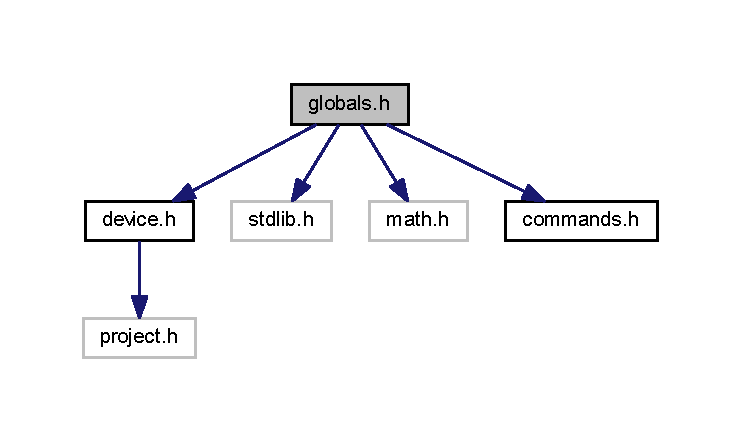
\includegraphics[width=350pt]{globals_8h__incl}
\end{center}
\end{figure}
This graph shows which files directly or indirectly include this file\+:
\nopagebreak
\begin{figure}[H]
\begin{center}
\leavevmode
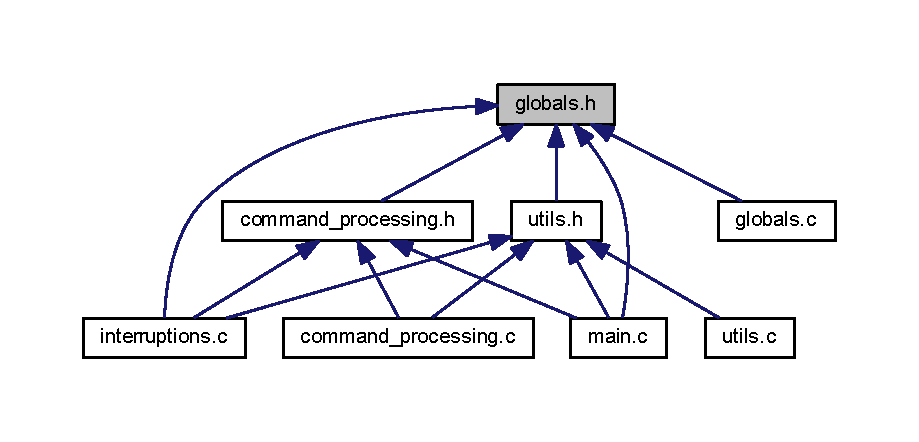
\includegraphics[width=350pt]{globals_8h__dep__incl}
\end{center}
\end{figure}
\subsection*{Data Structures}
\begin{DoxyCompactItemize}
\item 
struct \textbf{ st\+\_\+ref}
\begin{DoxyCompactList}\small\item\em Motor Reference structure. \end{DoxyCompactList}\item 
struct \textbf{ st\+\_\+meas}
\item 
struct \textbf{ st\+\_\+data}
\begin{DoxyCompactList}\small\item\em Data sent/received structure. \end{DoxyCompactList}\item 
struct \textbf{ st\+\_\+mem}
\item 
struct \textbf{ st\+\_\+dev}
\begin{DoxyCompactList}\small\item\em Device related structure. \end{DoxyCompactList}\item 
struct \textbf{ st\+\_\+calib}
\begin{DoxyCompactList}\small\item\em Hand calibration structure. \end{DoxyCompactList}\end{DoxyCompactItemize}
\subsection*{Macros}
\begin{DoxyCompactItemize}
\item 
\mbox{\label{globals_8h_a1c6d5de492ac61ad29aec7aa9a436bbf}} 
\#define {\bfseries V\+E\+R\+S\+I\+ON}~\char`\"{}SH-\/P\+RO v6.\+1.\+1 -\/ Master w/Rest position\char`\"{}
\item 
\#define \textbf{ N\+U\+M\+\_\+\+O\+F\+\_\+\+M\+O\+T\+O\+RS}~2
\item 
\#define \textbf{ N\+U\+M\+\_\+\+O\+F\+\_\+\+S\+E\+N\+S\+O\+RS}~3
\item 
\#define \textbf{ N\+U\+M\+\_\+\+O\+F\+\_\+\+E\+M\+GS}~2
\item 
\#define \textbf{ N\+U\+M\+\_\+\+O\+F\+\_\+\+A\+N\+A\+L\+O\+G\+\_\+\+I\+N\+P\+U\+TS}~4
\item 
\#define \textbf{ N\+U\+M\+\_\+\+O\+F\+\_\+\+P\+A\+R\+A\+MS}~25
\item 
\#define \textbf{ C\+A\+L\+I\+B\+R\+A\+T\+I\+O\+N\+\_\+\+D\+IV}~10
\item 
\mbox{\label{globals_8h_a14df76a41da04070ee775565e8d67e81}} 
\#define {\bfseries D\+I\+V\+\_\+\+I\+N\+I\+T\+\_\+\+V\+A\+L\+UE}~1
\item 
\mbox{\label{globals_8h_abf6c9afec04b86961e177e0646401ace}} 
\#define {\bfseries D\+M\+A\+\_\+\+B\+Y\+T\+E\+S\+\_\+\+P\+E\+R\+\_\+\+B\+U\+R\+ST}~2
\item 
\mbox{\label{globals_8h_ab4613f8bee68bc68fa6fe94a3ae6d568}} 
\#define {\bfseries D\+M\+A\+\_\+\+R\+E\+Q\+U\+E\+S\+T\+\_\+\+P\+E\+R\+\_\+\+B\+U\+R\+ST}~1
\item 
\mbox{\label{globals_8h_a3cc2eedb40809a1f15ad841c8abbcebf}} 
\#define {\bfseries D\+M\+A\+\_\+\+S\+R\+C\+\_\+\+B\+A\+SE}~(C\+Y\+D\+E\+V\+\_\+\+P\+E\+R\+I\+P\+H\+\_\+\+B\+A\+SE)
\item 
\mbox{\label{globals_8h_aa54e301f446a66cbf8c943d920c8e967}} 
\#define {\bfseries D\+M\+A\+\_\+\+D\+S\+T\+\_\+\+B\+A\+SE}~(C\+Y\+D\+E\+V\+\_\+\+S\+R\+A\+M\+\_\+\+B\+A\+SE)
\item 
\#define \textbf{ W\+A\+I\+T\+\_\+\+S\+T\+A\+RT}~0
\item 
\#define \textbf{ W\+A\+I\+T\+\_\+\+ID}~1
\item 
\#define \textbf{ W\+A\+I\+T\+\_\+\+L\+E\+N\+G\+TH}~2
\item 
\#define \textbf{ R\+E\+C\+E\+I\+VE}~3
\item 
\#define \textbf{ U\+N\+L\+O\+AD}~4
\item 
\mbox{\label{globals_8h_aa93f0eb578d23995850d61f7d61c55c1}} 
\#define {\bfseries F\+A\+L\+SE}~0
\item 
\mbox{\label{globals_8h_aa8cecfc5c5c054d2875c03e77b7be15d}} 
\#define {\bfseries T\+R\+UE}~1
\item 
\#define \textbf{ D\+E\+F\+A\+U\+L\+T\+\_\+\+E\+E\+P\+R\+O\+M\+\_\+\+D\+I\+S\+P\+L\+A\+C\+E\+M\+E\+NT}~8
\item 
\#define \textbf{ M\+A\+X\+\_\+\+W\+A\+T\+C\+H\+D\+O\+G\+\_\+\+T\+I\+M\+ER}~250
\item 
\#define \textbf{ P\+W\+M\+\_\+\+M\+A\+X\+\_\+\+V\+A\+L\+UE}~100
\item 
\#define \textbf{ A\+N\+T\+I\+\_\+\+W\+I\+N\+D\+UP}~1000
\item 
\#define \textbf{ D\+E\+F\+A\+U\+L\+T\+\_\+\+C\+U\+R\+R\+E\+N\+T\+\_\+\+L\+I\+M\+IT}~1000
\item 
\#define \textbf{ C\+U\+R\+R\+E\+N\+T\+\_\+\+H\+Y\+S\+T\+E\+R\+E\+S\+IS}~10
\item 
\#define \textbf{ E\+M\+G\+\_\+\+S\+A\+M\+P\+L\+E\+\_\+\+T\+O\+\_\+\+D\+I\+S\+C\+A\+RD}~500
\item 
\#define \textbf{ S\+A\+M\+P\+L\+E\+S\+\_\+\+F\+O\+R\+\_\+\+M\+E\+AN}~100
\item 
\#define \textbf{ S\+A\+M\+P\+L\+E\+S\+\_\+\+F\+O\+R\+\_\+\+E\+M\+G\+\_\+\+M\+E\+AN}~1000
\item 
\mbox{\label{globals_8h_a373fe6bcff3bcd2f3c47359f9e640bf5}} 
\#define {\bfseries C\+A\+L\+I\+B\+\_\+\+D\+E\+C\+I\+M\+A\+T\+I\+ON}~1
\item 
\mbox{\label{globals_8h_a3132fbe7ff2f1850f96481fca447326a}} 
\#define {\bfseries N\+U\+M\+\_\+\+O\+F\+\_\+\+C\+L\+O\+S\+U\+R\+ES}~5
\item 
\#define \textbf{ P\+O\+S\+\_\+\+I\+N\+T\+E\+G\+R\+A\+L\+\_\+\+S\+A\+T\+\_\+\+L\+I\+M\+IT}~50000000
\item 
\#define \textbf{ C\+U\+R\+R\+\_\+\+I\+N\+T\+E\+G\+R\+A\+L\+\_\+\+S\+A\+T\+\_\+\+L\+I\+M\+IT}~100000
\item 
\mbox{\label{globals_8h_a071576950e29c654790153cad12794cb}} 
\#define {\bfseries M\+I\+N\+\_\+\+C\+U\+R\+R\+\_\+\+S\+A\+T\+\_\+\+L\+I\+M\+IT}~30
\item 
\#define \textbf{ L\+O\+O\+K\+U\+P\+\_\+\+D\+IM}~6
\end{DoxyCompactItemize}
\subsection*{Enumerations}
\begin{DoxyCompactItemize}
\item 
enum \textbf{ emg\+\_\+status} \{ \newline
\textbf{ N\+O\+R\+M\+AL} = 0, 
\textbf{ R\+E\+S\+ET} = 1, 
\textbf{ D\+I\+S\+C\+A\+RD} = 2, 
\textbf{ S\+U\+M\+\_\+\+A\+N\+D\+\_\+\+M\+E\+AN} = 3, 
\newline
\textbf{ W\+A\+IT} = 4, 
\textbf{ W\+A\+I\+T\+\_\+\+EoC} = 5
 \}
\end{DoxyCompactItemize}
\subsection*{Variables}
\begin{DoxyCompactItemize}
\item 
struct \textbf{ st\+\_\+ref} g\+\_\+ref g\+\_\+ref\+New \textbf{ g\+\_\+ref\+Old}
\item 
struct \textbf{ st\+\_\+meas} g\+\_\+meas \textbf{ g\+\_\+meas\+Old}
\item 
struct \textbf{ st\+\_\+data} \textbf{ g\+\_\+rx}
\item 
struct \textbf{ st\+\_\+mem} g\+\_\+mem \textbf{ c\+\_\+mem}
\item 
\mbox{\label{globals_8h_aed96fdd8308fe2c4fc07c3b5db1c7bbb}} 
struct \textbf{ st\+\_\+calib} {\bfseries calib}
\item 
uint32 \textbf{ timer\+\_\+value}
\item 
uint32 \textbf{ timer\+\_\+value0}
\item 
int32 \textbf{ dev\+\_\+tension}
\item 
uint8 \textbf{ dev\+\_\+pwm\+\_\+limit}
\item 
int32 \textbf{ dev\+\_\+tension\+\_\+f}
\item 
\mbox{\label{globals_8h_a63d713ff9ac5ba0651f6af9115a32e4d}} 
int32 {\bfseries pow\+\_\+tension}
\item 
C\+Y\+B\+IT \textbf{ reset\+\_\+last\+\_\+value\+\_\+flag}
\item 
C\+Y\+B\+IT \textbf{ tension\+\_\+valid}
\item 
C\+Y\+B\+IT \textbf{ interrupt\+\_\+flag}
\item 
C\+Y\+B\+IT \textbf{ watchdog\+\_\+flag}
\item 
float \textbf{ tau\+\_\+feedback}
\item 
\mbox{\label{globals_8h_abb22f0a4462a0b4db27496654f2175a0}} 
int16 {\bfseries A\+D\+C\+\_\+buf} [4]
\item 
int8 \textbf{ pwm\+\_\+sign}
\item 
\mbox{\label{globals_8h_acf0e2a5d5954714103e295ac35513215}} 
uint8 {\bfseries master\+\_\+mode}
\item 
\mbox{\label{globals_8h_a1f8839fadee52a47a0042eaa695c3f3a}} 
uint8 {\bfseries rest\+\_\+enabled}
\item 
\mbox{\label{globals_8h_a0f13b80a0c329fa3176eb1e72ef36fb8}} 
uint8 {\bfseries forced\+\_\+open}
\item 
\mbox{\label{globals_8h_a485e5b90bbfb79aa97f874873cd6c93a}} 
int32 {\bfseries rest\+\_\+pos\+\_\+curr\+\_\+ref}
\item 
\mbox{\label{globals_8h_a50b50a565306d9a28c9e86694428a759}} 
uint8 {\bfseries receive\+\_\+meas\+\_\+from\+\_\+hand}
\item 
\mbox{\label{globals_8h_ab43d57397f71cb35c19d91058c48bed2}} 
int16 {\bfseries check2}
\item 
\mbox{\label{globals_8h_a07ae6981551bcb1232593903a0cec1be}} 
uint8 {\bfseries check3}
\item 
\mbox{\label{globals_8h_a57815d5e67537f44e37f31deb0cca84e}} 
uint8 {\bfseries check4}
\item 
\mbox{\label{globals_8h_a3e70f7fe645db3f664a6a47e63af6bff}} 
int32 {\bfseries check5}
\item 
\mbox{\label{globals_8h_ab2b7ed40fdef23f9dad3b7351df3b8f4}} 
int32 {\bfseries curr\+\_\+pos\+\_\+res}
\end{DoxyCompactItemize}


\subsection{Detailed Description}
Global definitions and macros are set in this file. 

\begin{DoxyDate}{Date}
June 06, 2016 
\end{DoxyDate}
\begin{DoxyAuthor}{Author}
{\itshape qbrobotics}, Mattia Poggiani 
\end{DoxyAuthor}
\begin{DoxyCopyright}{Copyright}
(C) 2012-\/2016 qbrobotics. All rights reserved. 

(C) 2017 Centro \char`\"{}\+E.\+Piaggio\char`\"{}. All rights reserved. 
\end{DoxyCopyright}


\subsection{Macro Definition Documentation}
\mbox{\label{globals_8h_a66edaed675ab232f06a4e5b3c30d101a}} 
\index{globals.\+h@{globals.\+h}!A\+N\+T\+I\+\_\+\+W\+I\+N\+D\+UP@{A\+N\+T\+I\+\_\+\+W\+I\+N\+D\+UP}}
\index{A\+N\+T\+I\+\_\+\+W\+I\+N\+D\+UP@{A\+N\+T\+I\+\_\+\+W\+I\+N\+D\+UP}!globals.\+h@{globals.\+h}}
\subsubsection{A\+N\+T\+I\+\_\+\+W\+I\+N\+D\+UP}
{\footnotesize\ttfamily \#define A\+N\+T\+I\+\_\+\+W\+I\+N\+D\+UP~1000}

Anti windup saturation. \mbox{\label{globals_8h_a80db2dce057c92400a7fb1678bc0b0a8}} 
\index{globals.\+h@{globals.\+h}!C\+A\+L\+I\+B\+R\+A\+T\+I\+O\+N\+\_\+\+D\+IV@{C\+A\+L\+I\+B\+R\+A\+T\+I\+O\+N\+\_\+\+D\+IV}}
\index{C\+A\+L\+I\+B\+R\+A\+T\+I\+O\+N\+\_\+\+D\+IV@{C\+A\+L\+I\+B\+R\+A\+T\+I\+O\+N\+\_\+\+D\+IV}!globals.\+h@{globals.\+h}}
\subsubsection{C\+A\+L\+I\+B\+R\+A\+T\+I\+O\+N\+\_\+\+D\+IV}
{\footnotesize\ttfamily \#define C\+A\+L\+I\+B\+R\+A\+T\+I\+O\+N\+\_\+\+D\+IV~10}

Frequency divisor for hand calibration (100\+Hz). \mbox{\label{globals_8h_a94ec4e208ccec9fc13d0f57094f6de35}} 
\index{globals.\+h@{globals.\+h}!C\+U\+R\+R\+\_\+\+I\+N\+T\+E\+G\+R\+A\+L\+\_\+\+S\+A\+T\+\_\+\+L\+I\+M\+IT@{C\+U\+R\+R\+\_\+\+I\+N\+T\+E\+G\+R\+A\+L\+\_\+\+S\+A\+T\+\_\+\+L\+I\+M\+IT}}
\index{C\+U\+R\+R\+\_\+\+I\+N\+T\+E\+G\+R\+A\+L\+\_\+\+S\+A\+T\+\_\+\+L\+I\+M\+IT@{C\+U\+R\+R\+\_\+\+I\+N\+T\+E\+G\+R\+A\+L\+\_\+\+S\+A\+T\+\_\+\+L\+I\+M\+IT}!globals.\+h@{globals.\+h}}
\subsubsection{C\+U\+R\+R\+\_\+\+I\+N\+T\+E\+G\+R\+A\+L\+\_\+\+S\+A\+T\+\_\+\+L\+I\+M\+IT}
{\footnotesize\ttfamily \#define C\+U\+R\+R\+\_\+\+I\+N\+T\+E\+G\+R\+A\+L\+\_\+\+S\+A\+T\+\_\+\+L\+I\+M\+IT~100000}

Anti windup on current control. \mbox{\label{globals_8h_ad03b1f5576bd45568413662f28b88d4e}} 
\index{globals.\+h@{globals.\+h}!C\+U\+R\+R\+E\+N\+T\+\_\+\+H\+Y\+S\+T\+E\+R\+E\+S\+IS@{C\+U\+R\+R\+E\+N\+T\+\_\+\+H\+Y\+S\+T\+E\+R\+E\+S\+IS}}
\index{C\+U\+R\+R\+E\+N\+T\+\_\+\+H\+Y\+S\+T\+E\+R\+E\+S\+IS@{C\+U\+R\+R\+E\+N\+T\+\_\+\+H\+Y\+S\+T\+E\+R\+E\+S\+IS}!globals.\+h@{globals.\+h}}
\subsubsection{C\+U\+R\+R\+E\+N\+T\+\_\+\+H\+Y\+S\+T\+E\+R\+E\+S\+IS}
{\footnotesize\ttfamily \#define C\+U\+R\+R\+E\+N\+T\+\_\+\+H\+Y\+S\+T\+E\+R\+E\+S\+IS~10}

milli\+Amperes of hysteresis for current control. \mbox{\label{globals_8h_ae0001cc59fb1ba0290c6ef8c2c5692d7}} 
\index{globals.\+h@{globals.\+h}!D\+E\+F\+A\+U\+L\+T\+\_\+\+C\+U\+R\+R\+E\+N\+T\+\_\+\+L\+I\+M\+IT@{D\+E\+F\+A\+U\+L\+T\+\_\+\+C\+U\+R\+R\+E\+N\+T\+\_\+\+L\+I\+M\+IT}}
\index{D\+E\+F\+A\+U\+L\+T\+\_\+\+C\+U\+R\+R\+E\+N\+T\+\_\+\+L\+I\+M\+IT@{D\+E\+F\+A\+U\+L\+T\+\_\+\+C\+U\+R\+R\+E\+N\+T\+\_\+\+L\+I\+M\+IT}!globals.\+h@{globals.\+h}}
\subsubsection{D\+E\+F\+A\+U\+L\+T\+\_\+\+C\+U\+R\+R\+E\+N\+T\+\_\+\+L\+I\+M\+IT}
{\footnotesize\ttfamily \#define D\+E\+F\+A\+U\+L\+T\+\_\+\+C\+U\+R\+R\+E\+N\+T\+\_\+\+L\+I\+M\+IT~1000}

Default Current limit, 0 stands for unlimited. \mbox{\label{globals_8h_a0f5a7e2ead9cd507bf8fc9a6f785f012}} 
\index{globals.\+h@{globals.\+h}!D\+E\+F\+A\+U\+L\+T\+\_\+\+E\+E\+P\+R\+O\+M\+\_\+\+D\+I\+S\+P\+L\+A\+C\+E\+M\+E\+NT@{D\+E\+F\+A\+U\+L\+T\+\_\+\+E\+E\+P\+R\+O\+M\+\_\+\+D\+I\+S\+P\+L\+A\+C\+E\+M\+E\+NT}}
\index{D\+E\+F\+A\+U\+L\+T\+\_\+\+E\+E\+P\+R\+O\+M\+\_\+\+D\+I\+S\+P\+L\+A\+C\+E\+M\+E\+NT@{D\+E\+F\+A\+U\+L\+T\+\_\+\+E\+E\+P\+R\+O\+M\+\_\+\+D\+I\+S\+P\+L\+A\+C\+E\+M\+E\+NT}!globals.\+h@{globals.\+h}}
\subsubsection{D\+E\+F\+A\+U\+L\+T\+\_\+\+E\+E\+P\+R\+O\+M\+\_\+\+D\+I\+S\+P\+L\+A\+C\+E\+M\+E\+NT}
{\footnotesize\ttfamily \#define D\+E\+F\+A\+U\+L\+T\+\_\+\+E\+E\+P\+R\+O\+M\+\_\+\+D\+I\+S\+P\+L\+A\+C\+E\+M\+E\+NT~8}

Number of pages occupied by the E\+E\+P\+R\+OM. \mbox{\label{globals_8h_a39897c457550afc048d5a251ba50c979}} 
\index{globals.\+h@{globals.\+h}!E\+M\+G\+\_\+\+S\+A\+M\+P\+L\+E\+\_\+\+T\+O\+\_\+\+D\+I\+S\+C\+A\+RD@{E\+M\+G\+\_\+\+S\+A\+M\+P\+L\+E\+\_\+\+T\+O\+\_\+\+D\+I\+S\+C\+A\+RD}}
\index{E\+M\+G\+\_\+\+S\+A\+M\+P\+L\+E\+\_\+\+T\+O\+\_\+\+D\+I\+S\+C\+A\+RD@{E\+M\+G\+\_\+\+S\+A\+M\+P\+L\+E\+\_\+\+T\+O\+\_\+\+D\+I\+S\+C\+A\+RD}!globals.\+h@{globals.\+h}}
\subsubsection{E\+M\+G\+\_\+\+S\+A\+M\+P\+L\+E\+\_\+\+T\+O\+\_\+\+D\+I\+S\+C\+A\+RD}
{\footnotesize\ttfamily \#define E\+M\+G\+\_\+\+S\+A\+M\+P\+L\+E\+\_\+\+T\+O\+\_\+\+D\+I\+S\+C\+A\+RD~500}

Number of sample to discard before calibration. \mbox{\label{globals_8h_a4f18d105a8fc18f649a92d96fb933eb3}} 
\index{globals.\+h@{globals.\+h}!L\+O\+O\+K\+U\+P\+\_\+\+D\+IM@{L\+O\+O\+K\+U\+P\+\_\+\+D\+IM}}
\index{L\+O\+O\+K\+U\+P\+\_\+\+D\+IM@{L\+O\+O\+K\+U\+P\+\_\+\+D\+IM}!globals.\+h@{globals.\+h}}
\subsubsection{L\+O\+O\+K\+U\+P\+\_\+\+D\+IM}
{\footnotesize\ttfamily \#define L\+O\+O\+K\+U\+P\+\_\+\+D\+IM~6}

Dimension of the current lookup table. \mbox{\label{globals_8h_a887dbd571d7f138cbe0e994e3fcc661b}} 
\index{globals.\+h@{globals.\+h}!M\+A\+X\+\_\+\+W\+A\+T\+C\+H\+D\+O\+G\+\_\+\+T\+I\+M\+ER@{M\+A\+X\+\_\+\+W\+A\+T\+C\+H\+D\+O\+G\+\_\+\+T\+I\+M\+ER}}
\index{M\+A\+X\+\_\+\+W\+A\+T\+C\+H\+D\+O\+G\+\_\+\+T\+I\+M\+ER@{M\+A\+X\+\_\+\+W\+A\+T\+C\+H\+D\+O\+G\+\_\+\+T\+I\+M\+ER}!globals.\+h@{globals.\+h}}
\subsubsection{M\+A\+X\+\_\+\+W\+A\+T\+C\+H\+D\+O\+G\+\_\+\+T\+I\+M\+ER}
{\footnotesize\ttfamily \#define M\+A\+X\+\_\+\+W\+A\+T\+C\+H\+D\+O\+G\+\_\+\+T\+I\+M\+ER~250}

num $\ast$ 2 [cs] \mbox{\label{globals_8h_a181be7cbd0b2da8e8bb809e6313bd67f}} 
\index{globals.\+h@{globals.\+h}!N\+U\+M\+\_\+\+O\+F\+\_\+\+A\+N\+A\+L\+O\+G\+\_\+\+I\+N\+P\+U\+TS@{N\+U\+M\+\_\+\+O\+F\+\_\+\+A\+N\+A\+L\+O\+G\+\_\+\+I\+N\+P\+U\+TS}}
\index{N\+U\+M\+\_\+\+O\+F\+\_\+\+A\+N\+A\+L\+O\+G\+\_\+\+I\+N\+P\+U\+TS@{N\+U\+M\+\_\+\+O\+F\+\_\+\+A\+N\+A\+L\+O\+G\+\_\+\+I\+N\+P\+U\+TS}!globals.\+h@{globals.\+h}}
\subsubsection{N\+U\+M\+\_\+\+O\+F\+\_\+\+A\+N\+A\+L\+O\+G\+\_\+\+I\+N\+P\+U\+TS}
{\footnotesize\ttfamily \#define N\+U\+M\+\_\+\+O\+F\+\_\+\+A\+N\+A\+L\+O\+G\+\_\+\+I\+N\+P\+U\+TS~4}

Total number of analogic inputs. \mbox{\label{globals_8h_a8e55cba7b8d4f9aa1eb36f311ce121e5}} 
\index{globals.\+h@{globals.\+h}!N\+U\+M\+\_\+\+O\+F\+\_\+\+E\+M\+GS@{N\+U\+M\+\_\+\+O\+F\+\_\+\+E\+M\+GS}}
\index{N\+U\+M\+\_\+\+O\+F\+\_\+\+E\+M\+GS@{N\+U\+M\+\_\+\+O\+F\+\_\+\+E\+M\+GS}!globals.\+h@{globals.\+h}}
\subsubsection{N\+U\+M\+\_\+\+O\+F\+\_\+\+E\+M\+GS}
{\footnotesize\ttfamily \#define N\+U\+M\+\_\+\+O\+F\+\_\+\+E\+M\+GS~2}

Number of emg channels. \mbox{\label{globals_8h_a39ac50737c1ee7d5b723b2597fdf6f26}} 
\index{globals.\+h@{globals.\+h}!N\+U\+M\+\_\+\+O\+F\+\_\+\+M\+O\+T\+O\+RS@{N\+U\+M\+\_\+\+O\+F\+\_\+\+M\+O\+T\+O\+RS}}
\index{N\+U\+M\+\_\+\+O\+F\+\_\+\+M\+O\+T\+O\+RS@{N\+U\+M\+\_\+\+O\+F\+\_\+\+M\+O\+T\+O\+RS}!globals.\+h@{globals.\+h}}
\subsubsection{N\+U\+M\+\_\+\+O\+F\+\_\+\+M\+O\+T\+O\+RS}
{\footnotesize\ttfamily \#define N\+U\+M\+\_\+\+O\+F\+\_\+\+M\+O\+T\+O\+RS~2}

Number of motors. \mbox{\label{globals_8h_aab4f4a0ece20c4bc27152bd72926d89c}} 
\index{globals.\+h@{globals.\+h}!N\+U\+M\+\_\+\+O\+F\+\_\+\+P\+A\+R\+A\+MS@{N\+U\+M\+\_\+\+O\+F\+\_\+\+P\+A\+R\+A\+MS}}
\index{N\+U\+M\+\_\+\+O\+F\+\_\+\+P\+A\+R\+A\+MS@{N\+U\+M\+\_\+\+O\+F\+\_\+\+P\+A\+R\+A\+MS}!globals.\+h@{globals.\+h}}
\subsubsection{N\+U\+M\+\_\+\+O\+F\+\_\+\+P\+A\+R\+A\+MS}
{\footnotesize\ttfamily \#define N\+U\+M\+\_\+\+O\+F\+\_\+\+P\+A\+R\+A\+MS~25}

Number of parameters saved in the E\+E\+P\+R\+OM \mbox{\label{globals_8h_af48a6b6fcdc5f5019fb108d03b07a727}} 
\index{globals.\+h@{globals.\+h}!N\+U\+M\+\_\+\+O\+F\+\_\+\+S\+E\+N\+S\+O\+RS@{N\+U\+M\+\_\+\+O\+F\+\_\+\+S\+E\+N\+S\+O\+RS}}
\index{N\+U\+M\+\_\+\+O\+F\+\_\+\+S\+E\+N\+S\+O\+RS@{N\+U\+M\+\_\+\+O\+F\+\_\+\+S\+E\+N\+S\+O\+RS}!globals.\+h@{globals.\+h}}
\subsubsection{N\+U\+M\+\_\+\+O\+F\+\_\+\+S\+E\+N\+S\+O\+RS}
{\footnotesize\ttfamily \#define N\+U\+M\+\_\+\+O\+F\+\_\+\+S\+E\+N\+S\+O\+RS~3}

Number of encoders. \mbox{\label{globals_8h_ad252b8b0421e545cce8ba0548a6ca4ed}} 
\index{globals.\+h@{globals.\+h}!P\+O\+S\+\_\+\+I\+N\+T\+E\+G\+R\+A\+L\+\_\+\+S\+A\+T\+\_\+\+L\+I\+M\+IT@{P\+O\+S\+\_\+\+I\+N\+T\+E\+G\+R\+A\+L\+\_\+\+S\+A\+T\+\_\+\+L\+I\+M\+IT}}
\index{P\+O\+S\+\_\+\+I\+N\+T\+E\+G\+R\+A\+L\+\_\+\+S\+A\+T\+\_\+\+L\+I\+M\+IT@{P\+O\+S\+\_\+\+I\+N\+T\+E\+G\+R\+A\+L\+\_\+\+S\+A\+T\+\_\+\+L\+I\+M\+IT}!globals.\+h@{globals.\+h}}
\subsubsection{P\+O\+S\+\_\+\+I\+N\+T\+E\+G\+R\+A\+L\+\_\+\+S\+A\+T\+\_\+\+L\+I\+M\+IT}
{\footnotesize\ttfamily \#define P\+O\+S\+\_\+\+I\+N\+T\+E\+G\+R\+A\+L\+\_\+\+S\+A\+T\+\_\+\+L\+I\+M\+IT~50000000}

Anti windup on position control. \mbox{\label{globals_8h_aafe0521fa22763b7afc50e12d31b450d}} 
\index{globals.\+h@{globals.\+h}!P\+W\+M\+\_\+\+M\+A\+X\+\_\+\+V\+A\+L\+UE@{P\+W\+M\+\_\+\+M\+A\+X\+\_\+\+V\+A\+L\+UE}}
\index{P\+W\+M\+\_\+\+M\+A\+X\+\_\+\+V\+A\+L\+UE@{P\+W\+M\+\_\+\+M\+A\+X\+\_\+\+V\+A\+L\+UE}!globals.\+h@{globals.\+h}}
\subsubsection{P\+W\+M\+\_\+\+M\+A\+X\+\_\+\+V\+A\+L\+UE}
{\footnotesize\ttfamily \#define P\+W\+M\+\_\+\+M\+A\+X\+\_\+\+V\+A\+L\+UE~100}

Maximum value of the P\+WM signal. \mbox{\label{globals_8h_a3b4d8a5e259fa47a909adefcda3bfb80}} 
\index{globals.\+h@{globals.\+h}!R\+E\+C\+E\+I\+VE@{R\+E\+C\+E\+I\+VE}}
\index{R\+E\+C\+E\+I\+VE@{R\+E\+C\+E\+I\+VE}!globals.\+h@{globals.\+h}}
\subsubsection{R\+E\+C\+E\+I\+VE}
{\footnotesize\ttfamily \#define R\+E\+C\+E\+I\+VE~3}

Package data receiving status \mbox{\label{globals_8h_a31532371c5c48fd2551639ed09afe4fb}} 
\index{globals.\+h@{globals.\+h}!S\+A\+M\+P\+L\+E\+S\+\_\+\+F\+O\+R\+\_\+\+E\+M\+G\+\_\+\+M\+E\+AN@{S\+A\+M\+P\+L\+E\+S\+\_\+\+F\+O\+R\+\_\+\+E\+M\+G\+\_\+\+M\+E\+AN}}
\index{S\+A\+M\+P\+L\+E\+S\+\_\+\+F\+O\+R\+\_\+\+E\+M\+G\+\_\+\+M\+E\+AN@{S\+A\+M\+P\+L\+E\+S\+\_\+\+F\+O\+R\+\_\+\+E\+M\+G\+\_\+\+M\+E\+AN}!globals.\+h@{globals.\+h}}
\subsubsection{S\+A\+M\+P\+L\+E\+S\+\_\+\+F\+O\+R\+\_\+\+E\+M\+G\+\_\+\+M\+E\+AN}
{\footnotesize\ttfamily \#define S\+A\+M\+P\+L\+E\+S\+\_\+\+F\+O\+R\+\_\+\+E\+M\+G\+\_\+\+M\+E\+AN~1000}

Number of samples used to mean emg values. \mbox{\label{globals_8h_a1f15a178b37117a29361e7ec20f77cc4}} 
\index{globals.\+h@{globals.\+h}!S\+A\+M\+P\+L\+E\+S\+\_\+\+F\+O\+R\+\_\+\+M\+E\+AN@{S\+A\+M\+P\+L\+E\+S\+\_\+\+F\+O\+R\+\_\+\+M\+E\+AN}}
\index{S\+A\+M\+P\+L\+E\+S\+\_\+\+F\+O\+R\+\_\+\+M\+E\+AN@{S\+A\+M\+P\+L\+E\+S\+\_\+\+F\+O\+R\+\_\+\+M\+E\+AN}!globals.\+h@{globals.\+h}}
\subsubsection{S\+A\+M\+P\+L\+E\+S\+\_\+\+F\+O\+R\+\_\+\+M\+E\+AN}
{\footnotesize\ttfamily \#define S\+A\+M\+P\+L\+E\+S\+\_\+\+F\+O\+R\+\_\+\+M\+E\+AN~100}

Number of samples used to mean current values. \mbox{\label{globals_8h_abf4aedd34d31b63b63061c975d872580}} 
\index{globals.\+h@{globals.\+h}!U\+N\+L\+O\+AD@{U\+N\+L\+O\+AD}}
\index{U\+N\+L\+O\+AD@{U\+N\+L\+O\+AD}!globals.\+h@{globals.\+h}}
\subsubsection{U\+N\+L\+O\+AD}
{\footnotesize\ttfamily \#define U\+N\+L\+O\+AD~4}

Package data flush status \mbox{\label{globals_8h_a6a6a0bb02e515a094c3e7ea1bcb66fcc}} 
\index{globals.\+h@{globals.\+h}!W\+A\+I\+T\+\_\+\+ID@{W\+A\+I\+T\+\_\+\+ID}}
\index{W\+A\+I\+T\+\_\+\+ID@{W\+A\+I\+T\+\_\+\+ID}!globals.\+h@{globals.\+h}}
\subsubsection{W\+A\+I\+T\+\_\+\+ID}
{\footnotesize\ttfamily \#define W\+A\+I\+T\+\_\+\+ID~1}

Package ID waiting status \mbox{\label{globals_8h_a235d2d0eac7e9af190ebafb84df37fd9}} 
\index{globals.\+h@{globals.\+h}!W\+A\+I\+T\+\_\+\+L\+E\+N\+G\+TH@{W\+A\+I\+T\+\_\+\+L\+E\+N\+G\+TH}}
\index{W\+A\+I\+T\+\_\+\+L\+E\+N\+G\+TH@{W\+A\+I\+T\+\_\+\+L\+E\+N\+G\+TH}!globals.\+h@{globals.\+h}}
\subsubsection{W\+A\+I\+T\+\_\+\+L\+E\+N\+G\+TH}
{\footnotesize\ttfamily \#define W\+A\+I\+T\+\_\+\+L\+E\+N\+G\+TH~2}

Package lenght waiting status \mbox{\label{globals_8h_aea55597952638136c7c929b238904c82}} 
\index{globals.\+h@{globals.\+h}!W\+A\+I\+T\+\_\+\+S\+T\+A\+RT@{W\+A\+I\+T\+\_\+\+S\+T\+A\+RT}}
\index{W\+A\+I\+T\+\_\+\+S\+T\+A\+RT@{W\+A\+I\+T\+\_\+\+S\+T\+A\+RT}!globals.\+h@{globals.\+h}}
\subsubsection{W\+A\+I\+T\+\_\+\+S\+T\+A\+RT}
{\footnotesize\ttfamily \#define W\+A\+I\+T\+\_\+\+S\+T\+A\+RT~0}

Package start waiting status 

\subsection{Enumeration Type Documentation}
\mbox{\label{globals_8h_a723f289c2be966c5e6c8dfe3d0b46f1e}} 
\index{globals.\+h@{globals.\+h}!emg\+\_\+status@{emg\+\_\+status}}
\index{emg\+\_\+status@{emg\+\_\+status}!globals.\+h@{globals.\+h}}
\subsubsection{emg\+\_\+status}
{\footnotesize\ttfamily enum \textbf{ emg\+\_\+status}}

\begin{DoxyEnumFields}{Enumerator}
\raisebox{\heightof{T}}[0pt][0pt]{\index{N\+O\+R\+M\+AL@{N\+O\+R\+M\+AL}!globals.\+h@{globals.\+h}}\index{globals.\+h@{globals.\+h}!N\+O\+R\+M\+AL@{N\+O\+R\+M\+AL}}}\mbox{\label{globals_8h_a723f289c2be966c5e6c8dfe3d0b46f1ea50d1448013c6f17125caee18aa418af7}} 
N\+O\+R\+M\+AL&Normal execution \\
\hline

\raisebox{\heightof{T}}[0pt][0pt]{\index{R\+E\+S\+ET@{R\+E\+S\+ET}!globals.\+h@{globals.\+h}}\index{globals.\+h@{globals.\+h}!R\+E\+S\+ET@{R\+E\+S\+ET}}}\mbox{\label{globals_8h_a723f289c2be966c5e6c8dfe3d0b46f1ea589b7d94a3d91d145720e2fed0eb3a05}} 
R\+E\+S\+ET&Reset analog measurements \\
\hline

\raisebox{\heightof{T}}[0pt][0pt]{\index{D\+I\+S\+C\+A\+RD@{D\+I\+S\+C\+A\+RD}!globals.\+h@{globals.\+h}}\index{globals.\+h@{globals.\+h}!D\+I\+S\+C\+A\+RD@{D\+I\+S\+C\+A\+RD}}}\mbox{\label{globals_8h_a723f289c2be966c5e6c8dfe3d0b46f1ea2c65e1f3e87da84f74b4fc2a908bf69d}} 
D\+I\+S\+C\+A\+RD&Discard first samples to obtain a correct value \\
\hline

\raisebox{\heightof{T}}[0pt][0pt]{\index{S\+U\+M\+\_\+\+A\+N\+D\+\_\+\+M\+E\+AN@{S\+U\+M\+\_\+\+A\+N\+D\+\_\+\+M\+E\+AN}!globals.\+h@{globals.\+h}}\index{globals.\+h@{globals.\+h}!S\+U\+M\+\_\+\+A\+N\+D\+\_\+\+M\+E\+AN@{S\+U\+M\+\_\+\+A\+N\+D\+\_\+\+M\+E\+AN}}}\mbox{\label{globals_8h_a723f289c2be966c5e6c8dfe3d0b46f1ea5bd42edcea28ad65a046391d8af6dfd8}} 
S\+U\+M\+\_\+\+A\+N\+D\+\_\+\+M\+E\+AN&Sum and mean a definite value of samples \\
\hline

\raisebox{\heightof{T}}[0pt][0pt]{\index{W\+A\+IT@{W\+A\+IT}!globals.\+h@{globals.\+h}}\index{globals.\+h@{globals.\+h}!W\+A\+IT@{W\+A\+IT}}}\mbox{\label{globals_8h_a723f289c2be966c5e6c8dfe3d0b46f1ea79a322ccb4b29b85b3cab52dbccefd17}} 
W\+A\+IT&The second emg waits until the first emg has a valid value \\
\hline

\raisebox{\heightof{T}}[0pt][0pt]{\index{W\+A\+I\+T\+\_\+\+EoC@{W\+A\+I\+T\+\_\+\+EoC}!globals.\+h@{globals.\+h}}\index{globals.\+h@{globals.\+h}!W\+A\+I\+T\+\_\+\+EoC@{W\+A\+I\+T\+\_\+\+EoC}}}\mbox{\label{globals_8h_a723f289c2be966c5e6c8dfe3d0b46f1ea81de86f7e28eb45b782fe4f79470575b}} 
W\+A\+I\+T\+\_\+\+EoC&The second emg waits for end of calibration \\
\hline

\end{DoxyEnumFields}


\subsection{Variable Documentation}
\mbox{\label{globals_8h_a44c3cbd8e234e0816f0334e29646a800}} 
\index{globals.\+h@{globals.\+h}!c\+\_\+mem@{c\+\_\+mem}}
\index{c\+\_\+mem@{c\+\_\+mem}!globals.\+h@{globals.\+h}}
\subsubsection{c\+\_\+mem}
{\footnotesize\ttfamily struct \textbf{ st\+\_\+mem} g\+\_\+mem c\+\_\+mem}

Memory parameters. \mbox{\label{globals_8h_a21f4f67e4203dea0b9956589eaa6cef3}} 
\index{globals.\+h@{globals.\+h}!dev\+\_\+pwm\+\_\+limit@{dev\+\_\+pwm\+\_\+limit}}
\index{dev\+\_\+pwm\+\_\+limit@{dev\+\_\+pwm\+\_\+limit}!globals.\+h@{globals.\+h}}
\subsubsection{dev\+\_\+pwm\+\_\+limit}
{\footnotesize\ttfamily uint8 dev\+\_\+pwm\+\_\+limit}

Device pwm limit \mbox{\label{globals_8h_a53a494e9edc739a4f7c884778d1a93b1}} 
\index{globals.\+h@{globals.\+h}!dev\+\_\+tension@{dev\+\_\+tension}}
\index{dev\+\_\+tension@{dev\+\_\+tension}!globals.\+h@{globals.\+h}}
\subsubsection{dev\+\_\+tension}
{\footnotesize\ttfamily int32 dev\+\_\+tension}

Power supply tension \mbox{\label{globals_8h_a600f1f02d397d3ffd8b03b8a4edace02}} 
\index{globals.\+h@{globals.\+h}!dev\+\_\+tension\+\_\+f@{dev\+\_\+tension\+\_\+f}}
\index{dev\+\_\+tension\+\_\+f@{dev\+\_\+tension\+\_\+f}!globals.\+h@{globals.\+h}}
\subsubsection{dev\+\_\+tension\+\_\+f}
{\footnotesize\ttfamily int32 dev\+\_\+tension\+\_\+f}

Filtered power supply tension \mbox{\label{globals_8h_a47c3980e6bddec492ca4315e36602ba0}} 
\index{globals.\+h@{globals.\+h}!g\+\_\+meas\+Old@{g\+\_\+meas\+Old}}
\index{g\+\_\+meas\+Old@{g\+\_\+meas\+Old}!globals.\+h@{globals.\+h}}
\subsubsection{g\+\_\+meas\+Old}
{\footnotesize\ttfamily struct \textbf{ st\+\_\+meas} g\+\_\+meas g\+\_\+meas\+Old}

Measurements. \mbox{\label{globals_8h_a158d26b6d15050b37d8039881d75e0dc}} 
\index{globals.\+h@{globals.\+h}!g\+\_\+ref\+Old@{g\+\_\+ref\+Old}}
\index{g\+\_\+ref\+Old@{g\+\_\+ref\+Old}!globals.\+h@{globals.\+h}}
\subsubsection{g\+\_\+ref\+Old}
{\footnotesize\ttfamily struct \textbf{ st\+\_\+ref} g\+\_\+ref g\+\_\+ref\+New g\+\_\+ref\+Old}

Reference variables. \mbox{\label{globals_8h_aa963ce8fafc11e104eb7ee22982d0345}} 
\index{globals.\+h@{globals.\+h}!g\+\_\+rx@{g\+\_\+rx}}
\index{g\+\_\+rx@{g\+\_\+rx}!globals.\+h@{globals.\+h}}
\subsubsection{g\+\_\+rx}
{\footnotesize\ttfamily struct \textbf{ st\+\_\+data} g\+\_\+rx}

Incoming/\+Outcoming data. \mbox{\label{globals_8h_a1e6fda88dfdabc63859f8907eb702920}} 
\index{globals.\+h@{globals.\+h}!interrupt\+\_\+flag@{interrupt\+\_\+flag}}
\index{interrupt\+\_\+flag@{interrupt\+\_\+flag}!globals.\+h@{globals.\+h}}
\subsubsection{interrupt\+\_\+flag}
{\footnotesize\ttfamily C\+Y\+B\+IT interrupt\+\_\+flag}

Interrupt flag enabler \mbox{\label{globals_8h_a8ac7ad7c894db750e93bc745818e26ca}} 
\index{globals.\+h@{globals.\+h}!pwm\+\_\+sign@{pwm\+\_\+sign}}
\index{pwm\+\_\+sign@{pwm\+\_\+sign}!globals.\+h@{globals.\+h}}
\subsubsection{pwm\+\_\+sign}
{\footnotesize\ttfamily int8 pwm\+\_\+sign}

A\+DC measurements buffer Sign of pwm driven. Used to obtain current sign. \mbox{\label{globals_8h_aa89a782cfe75ce7970236babd308fe69}} 
\index{globals.\+h@{globals.\+h}!reset\+\_\+last\+\_\+value\+\_\+flag@{reset\+\_\+last\+\_\+value\+\_\+flag}}
\index{reset\+\_\+last\+\_\+value\+\_\+flag@{reset\+\_\+last\+\_\+value\+\_\+flag}!globals.\+h@{globals.\+h}}
\subsubsection{reset\+\_\+last\+\_\+value\+\_\+flag}
{\footnotesize\ttfamily C\+Y\+B\+IT reset\+\_\+last\+\_\+value\+\_\+flag}

This flag is set when the encoders last values must be resetted. \mbox{\label{globals_8h_a894b799ffe45f442a6a897580ab7e98e}} 
\index{globals.\+h@{globals.\+h}!tau\+\_\+feedback@{tau\+\_\+feedback}}
\index{tau\+\_\+feedback@{tau\+\_\+feedback}!globals.\+h@{globals.\+h}}
\subsubsection{tau\+\_\+feedback}
{\footnotesize\ttfamily float tau\+\_\+feedback}

Torque feedback. \mbox{\label{globals_8h_ac42fa606610c2600210d9b7b2c1d0882}} 
\index{globals.\+h@{globals.\+h}!tension\+\_\+valid@{tension\+\_\+valid}}
\index{tension\+\_\+valid@{tension\+\_\+valid}!globals.\+h@{globals.\+h}}
\subsubsection{tension\+\_\+valid}
{\footnotesize\ttfamily C\+Y\+B\+IT tension\+\_\+valid}

Tension validation bit \mbox{\label{globals_8h_ad47cd0e4d0fcf5739a88e52e949a8084}} 
\index{globals.\+h@{globals.\+h}!timer\+\_\+value@{timer\+\_\+value}}
\index{timer\+\_\+value@{timer\+\_\+value}!globals.\+h@{globals.\+h}}
\subsubsection{timer\+\_\+value}
{\footnotesize\ttfamily uint32 timer\+\_\+value}

End time of the firmware main loop. \mbox{\label{globals_8h_a9bab7f1b1cf2ba38d5968eee42644c32}} 
\index{globals.\+h@{globals.\+h}!timer\+\_\+value0@{timer\+\_\+value0}}
\index{timer\+\_\+value0@{timer\+\_\+value0}!globals.\+h@{globals.\+h}}
\subsubsection{timer\+\_\+value0}
{\footnotesize\ttfamily uint32 timer\+\_\+value0}

Start time of the firmware main loop \mbox{\label{globals_8h_a156a860c465529ff2f515725ab816a58}} 
\index{globals.\+h@{globals.\+h}!watchdog\+\_\+flag@{watchdog\+\_\+flag}}
\index{watchdog\+\_\+flag@{watchdog\+\_\+flag}!globals.\+h@{globals.\+h}}
\subsubsection{watchdog\+\_\+flag}
{\footnotesize\ttfamily C\+Y\+B\+IT watchdog\+\_\+flag}

Watchdog flag enabler 
\doxysection{interruptions.\+c File Reference}
\label{interruptions_8c}\index{interruptions.c@{interruptions.c}}


Interruption handling and firmware core functions.  


{\ttfamily \#include $<$interruptions.\+h$>$}\newline
{\ttfamily \#include $<$command\+\_\+processing.\+h$>$}\newline
{\ttfamily \#include $<$globals.\+h$>$}\newline
{\ttfamily \#include $<$utils.\+h$>$}\newline
Include dependency graph for interruptions.\+c\+:
\nopagebreak
\begin{figure}[H]
\begin{center}
\leavevmode
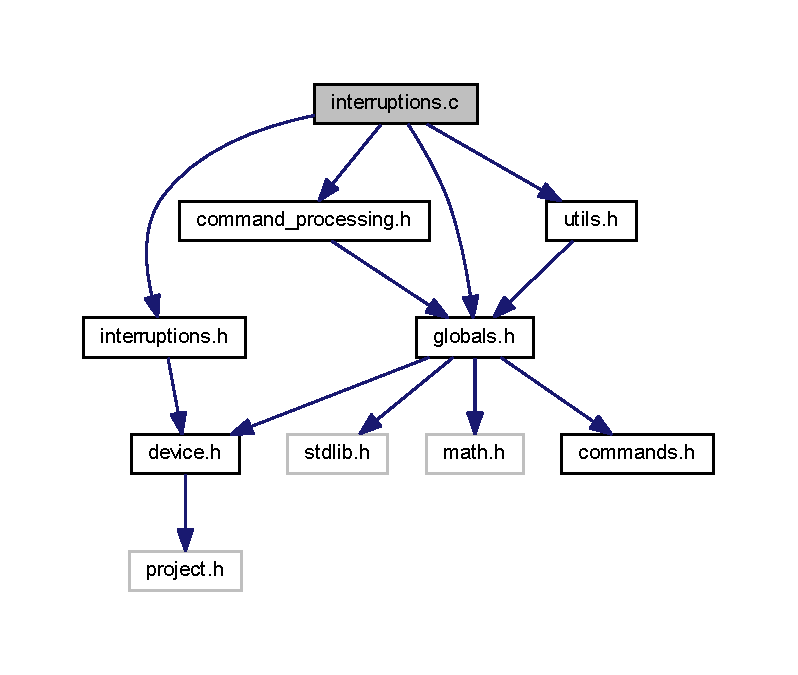
\includegraphics[width=350pt]{interruptions_8c__incl}
\end{center}
\end{figure}
\doxysubsection*{Functions}
\begin{DoxyCompactItemize}
\item 
\mbox{\label{interruptions_8c_a7692d8c3185943c5bdfaa6de0a172ad3}} 
{\bfseries CY\+\_\+\+ISR} (ISR\+\_\+\+RS485\+\_\+\+RX\+\_\+\+Ex\+Interrupt)
\item 
void \textbf{ interrupt\+\_\+manager} ()
\item 
void \textbf{ function\+\_\+scheduler} (void)
\item 
void \textbf{ motor\+\_\+control} ()
\item 
void \textbf{ analog\+\_\+read\+\_\+end} ()
\end{DoxyCompactItemize}


\doxysubsection{Detailed Description}
Interruption handling and firmware core functions. 

\begin{DoxyDate}{Date}
Feb 14th, 2023 
\end{DoxyDate}
\begin{DoxyAuthor}{Author}
{\itshape Centro \char`\"{}\+E.\+Piaggio\char`\"{}} 
\end{DoxyAuthor}
\begin{DoxyCopyright}{Copyright}
(C) 2012-\/2016 qbrobotics. All rights reserved. 

(C) 2017-\/2023 Centro \char`\"{}\+E.\+Piaggio\char`\"{}. All rights reserved. 
\end{DoxyCopyright}


\doxysubsection{Function Documentation}
\mbox{\label{interruptions_8c_a00a8d34962a63161405e5d7785b9625e}} 
\index{interruptions.c@{interruptions.c}!analog\_read\_end@{analog\_read\_end}}
\index{analog\_read\_end@{analog\_read\_end}!interruptions.c@{interruptions.c}}
\doxysubsubsection{analog\_read\_end()}
{\footnotesize\ttfamily void analog\+\_\+read\+\_\+end (\begin{DoxyParamCaption}{ }\end{DoxyParamCaption})}

This function executes and terminates the analog readings. \mbox{\label{interruptions_8c_a39df971c4e9f194be50c54dfd7aeabfe}} 
\index{interruptions.c@{interruptions.c}!function\_scheduler@{function\_scheduler}}
\index{function\_scheduler@{function\_scheduler}!interruptions.c@{interruptions.c}}
\doxysubsubsection{function\_scheduler()}
{\footnotesize\ttfamily void function\+\_\+scheduler (\begin{DoxyParamCaption}\item[{void}]{ }\end{DoxyParamCaption})}

This function schedules the other functions in an order that optimizes the controller usage. ~\newline
 \mbox{\label{interruptions_8c_a9790811526002d99b25a814afd02cbae}} 
\index{interruptions.c@{interruptions.c}!interrupt\_manager@{interrupt\_manager}}
\index{interrupt\_manager@{interrupt\_manager}!interruptions.c@{interruptions.c}}
\doxysubsubsection{interrupt\_manager()}
{\footnotesize\ttfamily void interrupt\+\_\+manager (\begin{DoxyParamCaption}{ }\end{DoxyParamCaption})}

This function is called in predefinited moments during firmware execution in order to unpack the received package. \mbox{\label{interruptions_8c_a8c7c487a5a127331b0de53443e3ca964}} 
\index{interruptions.c@{interruptions.c}!motor\_control@{motor\_control}}
\index{motor\_control@{motor\_control}!interruptions.c@{interruptions.c}}
\doxysubsubsection{motor\_control()}
{\footnotesize\ttfamily void motor\+\_\+control (\begin{DoxyParamCaption}{ }\end{DoxyParamCaption})}

This function controls the motor direction and velocity, depending on the input and control modality set. 

\doxysection{interruptions.\+h File Reference}
\label{interruptions_8h}\index{interruptions.h@{interruptions.h}}


Interruptions header file.  


{\ttfamily \#include $<$device.\+h$>$}\newline
Include dependency graph for interruptions.\+h\+:
\nopagebreak
\begin{figure}[H]
\begin{center}
\leavevmode
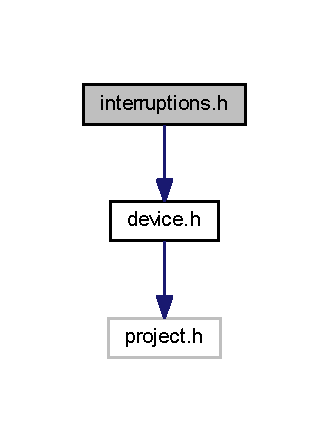
\includegraphics[width=158pt]{interruptions_8h__incl}
\end{center}
\end{figure}
This graph shows which files directly or indirectly include this file\+:
\nopagebreak
\begin{figure}[H]
\begin{center}
\leavevmode
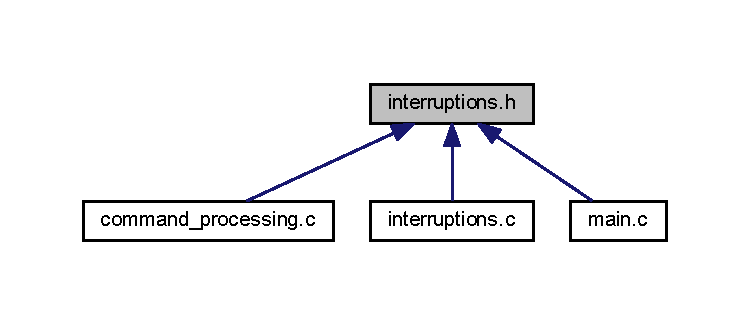
\includegraphics[width=350pt]{interruptions_8h__dep__incl}
\end{center}
\end{figure}
\doxysubsection*{Functions}
\begin{Indent}\textbf{ Interruptions}\par
\begin{DoxyCompactItemize}
\item 
\textbf{ CY\+\_\+\+ISR\+\_\+\+PROTO} (ISR\+\_\+\+RS485\+\_\+\+RX\+\_\+\+Ex\+Interrupt)
\end{DoxyCompactItemize}
\end{Indent}
\begin{Indent}\textbf{ General function scheduler}\par
\begin{DoxyCompactItemize}
\item 
void \textbf{ function\+\_\+scheduler} (void)
\end{DoxyCompactItemize}
\end{Indent}
\begin{Indent}\textbf{ Motor control function}\par
\begin{DoxyCompactItemize}
\item 
void \textbf{ motor\+\_\+control} ()
\end{DoxyCompactItemize}
\end{Indent}
\begin{Indent}\textbf{ Analog readings}\par
\begin{DoxyCompactItemize}
\item 
void \textbf{ analog\+\_\+read\+\_\+end} ()
\end{DoxyCompactItemize}
\end{Indent}
\begin{Indent}\textbf{ Interrupt manager}\par
\begin{DoxyCompactItemize}
\item 
void \textbf{ interrupt\+\_\+manager} ()
\end{DoxyCompactItemize}
\end{Indent}


\doxysubsection{Detailed Description}
Interruptions header file. 

\begin{DoxyDate}{Date}
Feb 14th, 2023 
\end{DoxyDate}
\begin{DoxyAuthor}{Author}
{\itshape Centro \char`\"{}\+E.\+Piaggio\char`\"{}} 
\end{DoxyAuthor}
\begin{DoxyCopyright}{Copyright}
(C) 2012-\/2016 qbrobotics. All rights reserved. 

(C) 2017-\/2023 Centro \char`\"{}\+E.\+Piaggio\char`\"{}. All rights reserved. 
\end{DoxyCopyright}


\doxysubsection{Function Documentation}
\mbox{\label{interruptions_8h_a00a8d34962a63161405e5d7785b9625e}} 
\index{interruptions.h@{interruptions.h}!analog\_read\_end@{analog\_read\_end}}
\index{analog\_read\_end@{analog\_read\_end}!interruptions.h@{interruptions.h}}
\doxysubsubsection{analog\_read\_end()}
{\footnotesize\ttfamily void analog\+\_\+read\+\_\+end (\begin{DoxyParamCaption}{ }\end{DoxyParamCaption})}

This function executes and terminates the analog readings. \mbox{\label{interruptions_8h_a7e24af8c83537b0441877bf0f00dd30a}} 
\index{interruptions.h@{interruptions.h}!CY\_ISR\_PROTO@{CY\_ISR\_PROTO}}
\index{CY\_ISR\_PROTO@{CY\_ISR\_PROTO}!interruptions.h@{interruptions.h}}
\doxysubsubsection{CY\_ISR\_PROTO()}
{\footnotesize\ttfamily CY\+\_\+\+ISR\+\_\+\+PROTO (\begin{DoxyParamCaption}\item[{ISR\+\_\+\+RS485\+\_\+\+RX\+\_\+\+Ex\+Interrupt}]{ }\end{DoxyParamCaption})}

This interruption sets a flag to let the firmware know that a communication interruption is pending and needs to be handled. The interruption will be handled in predefined moments during the firmware execution. When this interruption is handled, it unpacks the package received on the RS485 communication bus. ~\newline
 \mbox{\label{interruptions_8h_a39df971c4e9f194be50c54dfd7aeabfe}} 
\index{interruptions.h@{interruptions.h}!function\_scheduler@{function\_scheduler}}
\index{function\_scheduler@{function\_scheduler}!interruptions.h@{interruptions.h}}
\doxysubsubsection{function\_scheduler()}
{\footnotesize\ttfamily void function\+\_\+scheduler (\begin{DoxyParamCaption}\item[{void}]{ }\end{DoxyParamCaption})}

This function schedules the other functions in an order that optimizes the controller usage. ~\newline
 \mbox{\label{interruptions_8h_a9790811526002d99b25a814afd02cbae}} 
\index{interruptions.h@{interruptions.h}!interrupt\_manager@{interrupt\_manager}}
\index{interrupt\_manager@{interrupt\_manager}!interruptions.h@{interruptions.h}}
\doxysubsubsection{interrupt\_manager()}
{\footnotesize\ttfamily void interrupt\+\_\+manager (\begin{DoxyParamCaption}{ }\end{DoxyParamCaption})}

This function is called in predefinited moments during firmware execution in order to unpack the received package. \mbox{\label{interruptions_8h_a8c7c487a5a127331b0de53443e3ca964}} 
\index{interruptions.h@{interruptions.h}!motor\_control@{motor\_control}}
\index{motor\_control@{motor\_control}!interruptions.h@{interruptions.h}}
\doxysubsubsection{motor\_control()}
{\footnotesize\ttfamily void motor\+\_\+control (\begin{DoxyParamCaption}{ }\end{DoxyParamCaption})}

This function controls the motor direction and velocity, depending on the input and control modality set. 

\section{main.\+c File Reference}
\label{main_8c}\index{main.\+c@{main.\+c}}


Firmware main file.  


{\ttfamily \#include $<$device.\+h$>$}\newline
{\ttfamily \#include $<$globals.\+h$>$}\newline
{\ttfamily \#include $<$interruptions.\+h$>$}\newline
{\ttfamily \#include $<$command\+\_\+processing.\+h$>$}\newline
{\ttfamily \#include $<$utils.\+h$>$}\newline
Include dependency graph for main.\+c\+:
\nopagebreak
\begin{figure}[H]
\begin{center}
\leavevmode
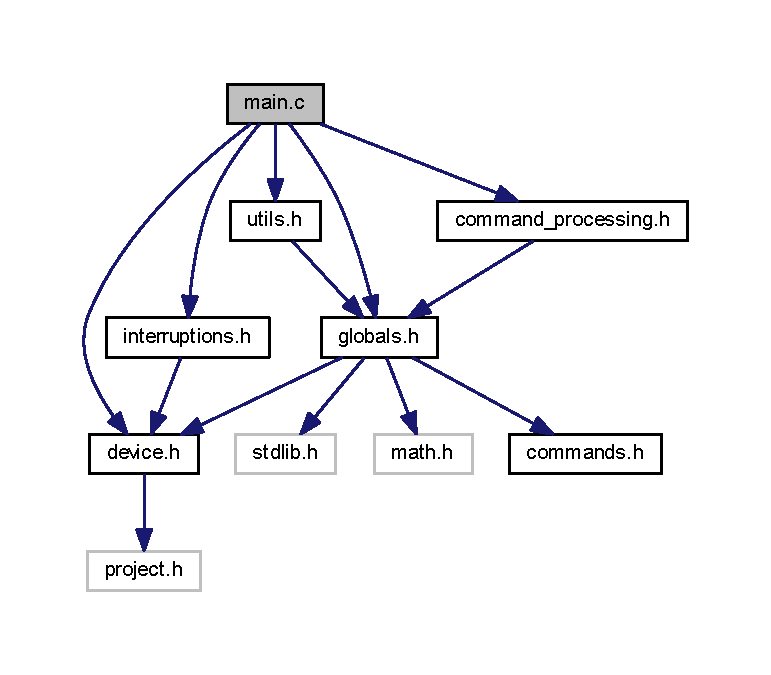
\includegraphics[width=350pt]{main_8c__incl}
\end{center}
\end{figure}
\subsection*{Functions}
\begin{DoxyCompactItemize}
\item 
\mbox{\label{main_8c_ae66f6b31b5ad750f1fe042a706a4e3d4}} 
int {\bfseries main} ()
\end{DoxyCompactItemize}


\subsection{Detailed Description}
Firmware main file. 

\begin{DoxyDate}{Date}
June 06, 2016 
\end{DoxyDate}
\begin{DoxyAuthor}{Author}
qbrobotics 
\end{DoxyAuthor}
\begin{DoxyCopyright}{Copyright}
(C) 2012-\/2016 qbrobotics. All rights reserved. 

(C) 2017 Centro \char`\"{}\+E.\+Piaggio\char`\"{}. All rights reserved. 
\end{DoxyCopyright}

\doxysection{utils.\+c File Reference}
\label{utils_8c}\index{utils.c@{utils.c}}


Definition of utility functions.  


{\ttfamily \#include $<$utils.\+h$>$}\newline
{\ttfamily \#include $<$math.\+h$>$}\newline
Include dependency graph for utils.\+c\+:
\nopagebreak
\begin{figure}[H]
\begin{center}
\leavevmode
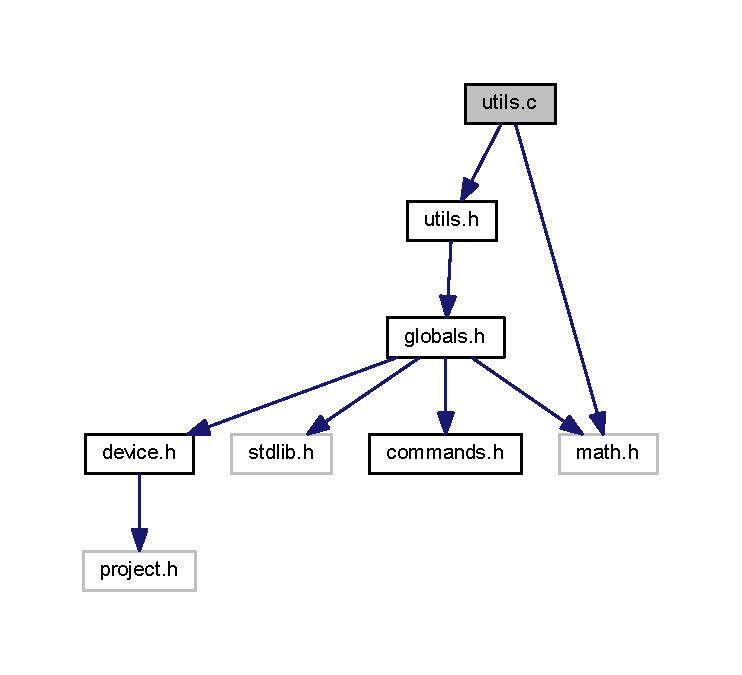
\includegraphics[width=350pt]{utils_8c__incl}
\end{center}
\end{figure}
\doxysubsection*{Macros}
\begin{DoxyCompactItemize}
\item 
\mbox{\label{utils_8c_abd7b39be02bc15d79b73e5cf2b531299}} 
\#define {\bfseries N1}~15
\begin{DoxyCompactList}\small\item\em Teeth of the first encoder wheel. \end{DoxyCompactList}\item 
\mbox{\label{utils_8c_acd864640121c7df2c19f61f7baa507e4}} 
\#define {\bfseries N2}~14
\begin{DoxyCompactList}\small\item\em Teeth of the second encoder wheel. \end{DoxyCompactList}\item 
\mbox{\label{utils_8c_ae7dee1f3e548d0fefe0f67c994de03e4}} 
\#define {\bfseries I1}~1
\begin{DoxyCompactList}\small\item\em First wheel invariant value. \end{DoxyCompactList}\item 
\mbox{\label{utils_8c_a964f933e75944a909cc698a3997c8f14}} 
\#define {\bfseries I2}~(-\/1)
\begin{DoxyCompactList}\small\item\em Second wheel invariant value. \end{DoxyCompactList}\item 
\mbox{\label{utils_8c_a52037c938e3c1b126c6277da5ca689d0}} 
\#define {\bfseries M}~65536
\begin{DoxyCompactList}\small\item\em Number of encoder ticks per turn. \end{DoxyCompactList}\end{DoxyCompactItemize}
\doxysubsection*{Functions}
\begin{DoxyCompactItemize}
\item 
int32 \textbf{ filter\+\_\+v} (int32 new\+\_\+value)
\item 
int32 \textbf{ filter\+\_\+i1} (int32 new\+\_\+value)
\item 
int32 \textbf{ filter\+\_\+ch1} (int32 new\+\_\+value)
\item 
int32 \textbf{ filter\+\_\+ch2} (int32 new\+\_\+value)
\item 
int32 \textbf{ filter\+\_\+vel\+\_\+1} (int32 new\+\_\+value)
\item 
int32 \textbf{ filter\+\_\+vel\+\_\+2} (int32 new\+\_\+value)
\item 
int32 \textbf{ filter\+\_\+vel\+\_\+3} (int32 new\+\_\+value)
\item 
int32 \textbf{ filter\+\_\+acc\+\_\+1} (int32 new\+\_\+value)
\item 
int32 \textbf{ filter\+\_\+acc\+\_\+2} (int32 new\+\_\+value)
\item 
int32 \textbf{ filter\+\_\+acc\+\_\+3} (int32 new\+\_\+value)
\item 
int32 \textbf{ filter\+\_\+voltage} (int32 new\+\_\+value)
\item 
CYBIT \textbf{ check\+\_\+enc\+\_\+data} (const uint32 $\ast$value)
\item 
int \textbf{ my\+\_\+round} (const double x)
\item 
uint32 \textbf{ my\+\_\+mod} (int32 val, int32 divisor)
\item 
void \textbf{ calibration} (void)
\item 
int \textbf{ calc\+\_\+turns\+\_\+fcn} (const int32 pos1, const int32 pos2)
\item 
void \textbf{ check\+\_\+rest\+\_\+position} (void)
\end{DoxyCompactItemize}


\doxysubsection{Detailed Description}
Definition of utility functions. 

\begin{DoxyDate}{Date}
October 01, 2017 
\end{DoxyDate}
\begin{DoxyAuthor}{Author}
{\itshape Centro \char`\"{}\+E.\+Piaggio\char`\"{}} 
\end{DoxyAuthor}
\begin{DoxyCopyright}{Copyright}
(C) 2012-\/2016 qbrobotics. All rights reserved. 

(C) 2017 Centro \char`\"{}\+E.\+Piaggio\char`\"{}. All rights reserved. 
\end{DoxyCopyright}


\doxysubsection{Function Documentation}
\mbox{\label{utils_8c_afa68f255d25478e463690f63d529c29d}} 
\index{utils.c@{utils.c}!calc\_turns\_fcn@{calc\_turns\_fcn}}
\index{calc\_turns\_fcn@{calc\_turns\_fcn}!utils.c@{utils.c}}
\doxysubsubsection{calc\_turns\_fcn()}
{\footnotesize\ttfamily int calc\+\_\+turns\+\_\+fcn (\begin{DoxyParamCaption}\item[{const int32}]{pos1,  }\item[{const int32}]{pos2 }\end{DoxyParamCaption})}

This function is used at startup to reconstruct the correct turn of the shaft connected to the motor. It need two encoders to work.


\begin{DoxyParams}{Parameters}
{\em pos1} & First encoder position \\
\hline
{\em pos2} & Second encoder position\\
\hline
\end{DoxyParams}
\begin{DoxyReturn}{Returns}
Returns the number of turns of motor pulley at startup 
\end{DoxyReturn}
\mbox{\label{utils_8c_a0b6a0b24c6bd8af032a6778166201f7e}} 
\index{utils.c@{utils.c}!calibration@{calibration}}
\index{calibration@{calibration}!utils.c@{utils.c}}
\doxysubsubsection{calibration()}
{\footnotesize\ttfamily void calibration (\begin{DoxyParamCaption}{ }\end{DoxyParamCaption})}

This function counts a series of hand opening and closing used to execute a calibration of the device. \mbox{\label{utils_8c_ae7faec5b3a1d000c90f70abfc1dfca92}} 
\index{utils.c@{utils.c}!check\_enc\_data@{check\_enc\_data}}
\index{check\_enc\_data@{check\_enc\_data}!utils.c@{utils.c}}
\doxysubsubsection{check\_enc\_data()}
{\footnotesize\ttfamily CYBIT check\+\_\+enc\+\_\+data (\begin{DoxyParamCaption}\item[{const uint32 $\ast$}]{value }\end{DoxyParamCaption})}

This function controls if the read encoder data is correct or not.


\begin{DoxyParams}{Parameters}
{\em value} & A pointer to the encoder data read\\
\hline
\end{DoxyParams}
\begin{DoxyReturn}{Returns}
Returns 1 if the read data is correct, 0 otherwise ~\newline
 
\end{DoxyReturn}
\mbox{\label{utils_8c_a13fca172b37b6f76749a864c1439b497}} 
\index{utils.c@{utils.c}!check\_rest\_position@{check\_rest\_position}}
\index{check\_rest\_position@{check\_rest\_position}!utils.c@{utils.c}}
\doxysubsubsection{check\_rest\_position()}
{\footnotesize\ttfamily void check\+\_\+rest\+\_\+position (\begin{DoxyParamCaption}{ }\end{DoxyParamCaption})}

This function checks for rest position and, in case, gives a position reference to the hand. \mbox{\label{utils_8c_ac13ce27c5d07ec4a8dd7d664619e13e8}} 
\index{utils.c@{utils.c}!filter\_acc\_1@{filter\_acc\_1}}
\index{filter\_acc\_1@{filter\_acc\_1}!utils.c@{utils.c}}
\doxysubsubsection{filter\_acc\_1()}
{\footnotesize\ttfamily int32 filter\+\_\+acc\+\_\+1 (\begin{DoxyParamCaption}\item[{int32}]{value }\end{DoxyParamCaption})}

Filter on first encoder rotational acceleration. The weighted average between the old value and the new one is executed.


\begin{DoxyParams}{Parameters}
{\em value} & New value of the filter.\\
\hline
\end{DoxyParams}
\begin{DoxyReturn}{Returns}
Returns the filtered first encoder rotational acceleration value 
\end{DoxyReturn}
\mbox{\label{utils_8c_a8578af55dde4ea39bb3525b417ff82e2}} 
\index{utils.c@{utils.c}!filter\_acc\_2@{filter\_acc\_2}}
\index{filter\_acc\_2@{filter\_acc\_2}!utils.c@{utils.c}}
\doxysubsubsection{filter\_acc\_2()}
{\footnotesize\ttfamily int32 filter\+\_\+acc\+\_\+2 (\begin{DoxyParamCaption}\item[{int32}]{value }\end{DoxyParamCaption})}

Filter on second encoder rotation acceleration (if present). The weighted average between the old value and the new one is executed.


\begin{DoxyParams}{Parameters}
{\em value} & New value of the filter.\\
\hline
\end{DoxyParams}
\begin{DoxyReturn}{Returns}
Returns the filtered second encoder rotational acceleration value 
\end{DoxyReturn}
\mbox{\label{utils_8c_afbd3d0d191893b101de61bea2b04d7f2}} 
\index{utils.c@{utils.c}!filter\_acc\_3@{filter\_acc\_3}}
\index{filter\_acc\_3@{filter\_acc\_3}!utils.c@{utils.c}}
\doxysubsubsection{filter\_acc\_3()}
{\footnotesize\ttfamily int32 filter\+\_\+acc\+\_\+3 (\begin{DoxyParamCaption}\item[{int32}]{value }\end{DoxyParamCaption})}

Filter on third encoder rotation acceleration (if present). The weighted average between the old value and the new one is executed.


\begin{DoxyParams}{Parameters}
{\em value} & New value of the filter.\\
\hline
\end{DoxyParams}
\begin{DoxyReturn}{Returns}
Returns the filtered third encoder rotational acceleration value 
\end{DoxyReturn}
\mbox{\label{utils_8c_a9bed4948a884d80dc0d3511648e8eef3}} 
\index{utils.c@{utils.c}!filter\_ch1@{filter\_ch1}}
\index{filter\_ch1@{filter\_ch1}!utils.c@{utils.c}}
\doxysubsubsection{filter\_ch1()}
{\footnotesize\ttfamily int32 filter\+\_\+ch1 (\begin{DoxyParamCaption}\item[{int32}]{value }\end{DoxyParamCaption})}

Filter on the first EMG sensor converted value. The weighted average between the old value and the new one is executed.


\begin{DoxyParams}{Parameters}
{\em value} & New value of the filter.\\
\hline
\end{DoxyParams}
\begin{DoxyReturn}{Returns}
Returns the filtered emg sensor value 
\end{DoxyReturn}
\mbox{\label{utils_8c_a66c5359b055eac4ae46c8146a9c45730}} 
\index{utils.c@{utils.c}!filter\_ch2@{filter\_ch2}}
\index{filter\_ch2@{filter\_ch2}!utils.c@{utils.c}}
\doxysubsubsection{filter\_ch2()}
{\footnotesize\ttfamily int32 filter\+\_\+ch2 (\begin{DoxyParamCaption}\item[{int32}]{value }\end{DoxyParamCaption})}

Filter on the second EMG sensor converted value. The weighted average between the old value and the new one is executed.


\begin{DoxyParams}{Parameters}
{\em value} & New value of the filter.\\
\hline
\end{DoxyParams}
\begin{DoxyReturn}{Returns}
Returns the filtered emg sensor value 
\end{DoxyReturn}
\mbox{\label{utils_8c_ad3131df52849d030b02010f285481ba6}} 
\index{utils.c@{utils.c}!filter\_i1@{filter\_i1}}
\index{filter\_i1@{filter\_i1}!utils.c@{utils.c}}
\doxysubsubsection{filter\_i1()}
{\footnotesize\ttfamily int32 filter\+\_\+i1 (\begin{DoxyParamCaption}\item[{int32}]{value }\end{DoxyParamCaption})}

Filter on the motor current converted value. The weighted average between the old value and the new one is executed.


\begin{DoxyParams}{Parameters}
{\em value} & New value of the filter.\\
\hline
\end{DoxyParams}
\begin{DoxyReturn}{Returns}
Returns the filtered current value 
\end{DoxyReturn}
\mbox{\label{utils_8c_af034fe9aa479d4adfc6e75e20b2f7ff3}} 
\index{utils.c@{utils.c}!filter\_v@{filter\_v}}
\index{filter\_v@{filter\_v}!utils.c@{utils.c}}
\doxysubsubsection{filter\_v()}
{\footnotesize\ttfamily int32 filter\+\_\+v (\begin{DoxyParamCaption}\item[{int32}]{new\+\_\+value }\end{DoxyParamCaption})}

Filter on the converted voltage value. The weighted average between the old value and the new one is executed.


\begin{DoxyParams}{Parameters}
{\em new\+\_\+value} & New value of the filter.\\
\hline
\end{DoxyParams}
\begin{DoxyReturn}{Returns}
Returns the filtered voltage value 
\end{DoxyReturn}
\mbox{\label{utils_8c_a19d6395ebc48dcac09068a5c6eb19596}} 
\index{utils.c@{utils.c}!filter\_vel\_1@{filter\_vel\_1}}
\index{filter\_vel\_1@{filter\_vel\_1}!utils.c@{utils.c}}
\doxysubsubsection{filter\_vel\_1()}
{\footnotesize\ttfamily int32 filter\+\_\+vel\+\_\+1 (\begin{DoxyParamCaption}\item[{int32}]{value }\end{DoxyParamCaption})}

Filter on first encoder rotational speed. The weighted average between the old value and the new one is executed.


\begin{DoxyParams}{Parameters}
{\em value} & New value of the filter.\\
\hline
\end{DoxyParams}
\begin{DoxyReturn}{Returns}
Returns the filtered first encoder rotational speed value 
\end{DoxyReturn}
\mbox{\label{utils_8c_aa24da14909e1e213a2d5f5522752f2c9}} 
\index{utils.c@{utils.c}!filter\_vel\_2@{filter\_vel\_2}}
\index{filter\_vel\_2@{filter\_vel\_2}!utils.c@{utils.c}}
\doxysubsubsection{filter\_vel\_2()}
{\footnotesize\ttfamily int32 filter\+\_\+vel\+\_\+2 (\begin{DoxyParamCaption}\item[{int32}]{value }\end{DoxyParamCaption})}

Filter on second encoder rotational speed (if present). The weighted average between the old value and the new one is executed.


\begin{DoxyParams}{Parameters}
{\em value} & New value of the filter.\\
\hline
\end{DoxyParams}
\begin{DoxyReturn}{Returns}
Returns the filtered second encoder rotational speed value 
\end{DoxyReturn}
\mbox{\label{utils_8c_a44d5627a5b0d37a70edddad83a3362ea}} 
\index{utils.c@{utils.c}!filter\_vel\_3@{filter\_vel\_3}}
\index{filter\_vel\_3@{filter\_vel\_3}!utils.c@{utils.c}}
\doxysubsubsection{filter\_vel\_3()}
{\footnotesize\ttfamily int32 filter\+\_\+vel\+\_\+3 (\begin{DoxyParamCaption}\item[{int32}]{value }\end{DoxyParamCaption})}

Filter on third encoder rotational speed (if present). The weighted average between the old value and the new one is executed.


\begin{DoxyParams}{Parameters}
{\em value} & New value of the filter.\\
\hline
\end{DoxyParams}
\begin{DoxyReturn}{Returns}
Returns the filtered third encoder rotational speed value 
\end{DoxyReturn}
\mbox{\label{utils_8c_ae34079960d1cb2d36ceb390569507710}} 
\index{utils.c@{utils.c}!filter\_voltage@{filter\_voltage}}
\index{filter\_voltage@{filter\_voltage}!utils.c@{utils.c}}
\doxysubsubsection{filter\_voltage()}
{\footnotesize\ttfamily int32 filter\+\_\+voltage (\begin{DoxyParamCaption}\item[{int32}]{value }\end{DoxyParamCaption})}

Filter on voltage readings. The weighted average between the old value and the new one is executed.


\begin{DoxyParams}{Parameters}
{\em value} & New value of the filter.\\
\hline
\end{DoxyParams}
\begin{DoxyReturn}{Returns}
Returns the filtered voltage value 
\end{DoxyReturn}
\mbox{\label{utils_8c_a01d3bb6c1fd469a6c530fb296e4fe0fe}} 
\index{utils.c@{utils.c}!my\_mod@{my\_mod}}
\index{my\_mod@{my\_mod}!utils.c@{utils.c}}
\doxysubsubsection{my\_mod()}
{\footnotesize\ttfamily uint32 my\+\_\+mod (\begin{DoxyParamCaption}\item[{int32}]{val,  }\item[{int32}]{divisor }\end{DoxyParamCaption})}

This function computes the module function, returning positive values regardless of wheter the value passed is negative


\begin{DoxyParams}{Parameters}
{\em val} & The value of which the module needs to be calculated \\
\hline
{\em divisor} & The divisor according to which the module is calculated \\
\hline
\end{DoxyParams}
\mbox{\label{utils_8c_a1ea4108a2c530470624ce2678e65dcef}} 
\index{utils.c@{utils.c}!my\_round@{my\_round}}
\index{my\_round@{my\_round}!utils.c@{utils.c}}
\doxysubsubsection{my\_round()}
{\footnotesize\ttfamily int my\+\_\+round (\begin{DoxyParamCaption}\item[{const double}]{x }\end{DoxyParamCaption})}

This functions approximates the value passed to the nearest integer


\begin{DoxyParams}{Parameters}
{\em x} & The floating point value that needs to be rounded \\
\hline
\end{DoxyParams}

\section{utils.\+h File Reference}
\label{utils_8h}\index{utils.\+h@{utils.\+h}}


Utility functions declaration.  


{\ttfamily \#include $<$globals.\+h$>$}\newline
Include dependency graph for utils.\+h\+:
\nopagebreak
\begin{figure}[H]
\begin{center}
\leavevmode
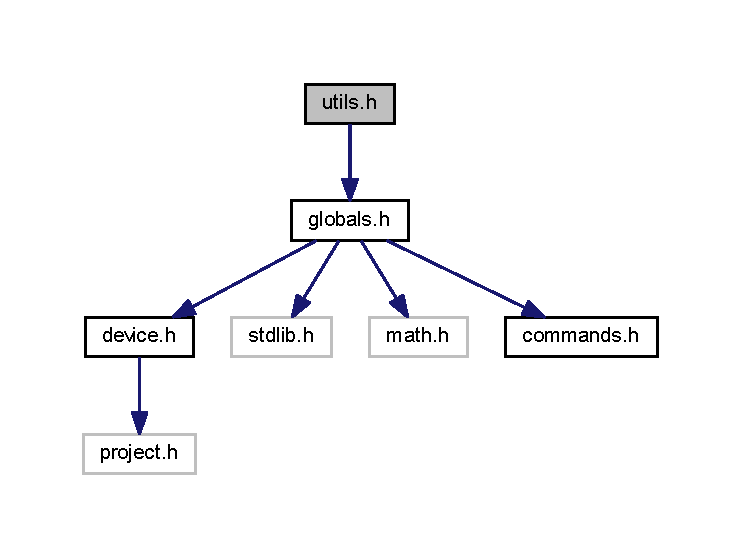
\includegraphics[width=350pt]{utils_8h__incl}
\end{center}
\end{figure}
This graph shows which files directly or indirectly include this file\+:\nopagebreak
\begin{figure}[H]
\begin{center}
\leavevmode
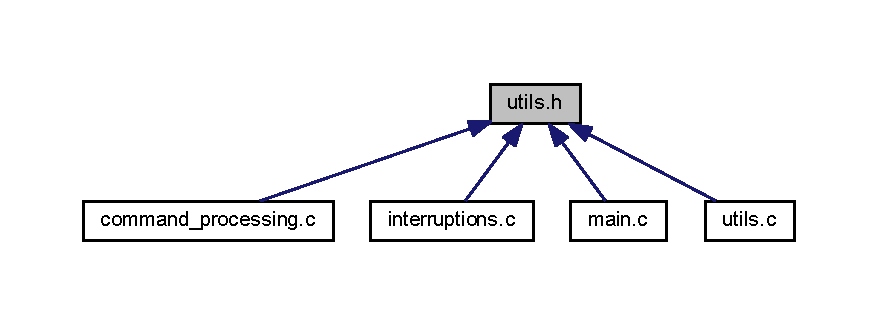
\includegraphics[width=350pt]{utils_8h__dep__incl}
\end{center}
\end{figure}
\subsection*{Macros}
\begin{DoxyCompactItemize}
\item 
\mbox{\label{utils_8h_a05ec5d63e2ba7621d706137124efca7d}} 
\#define {\bfseries T\+I\+M\+E\+R\+\_\+\+C\+L\+O\+CK}~10000
\item 
\mbox{\label{utils_8h_af5abd28c44c29b7397c84f1fec4b1d84}} 
\#define \textbf{ A\+L\+P\+HA}~32
\begin{DoxyCompactList}\small\item\em Voltage and current filters constant. \end{DoxyCompactList}\item 
\mbox{\label{utils_8h_a1b996515309fc3c03449912bb33046e3}} 
\#define \textbf{ B\+E\+TA}~50
\begin{DoxyCompactList}\small\item\em Emg filters constant. \end{DoxyCompactList}\item 
\mbox{\label{utils_8h_a8659b9de3e544ff142b153b076f30fd5}} 
\#define \textbf{ G\+A\+M\+MA}~32
\begin{DoxyCompactList}\small\item\em Velocity filters constant. \end{DoxyCompactList}\item 
\mbox{\label{utils_8h_a3fd2b1bcd7ddcf506237987ad780f495}} 
\#define \textbf{ D\+E\+L\+TA}~32
\begin{DoxyCompactList}\small\item\em Acceleration filters constant. \end{DoxyCompactList}\item 
\mbox{\label{utils_8h_a002b2f4894492820fe708b1b7e7c5e70}} 
\#define \textbf{ E\+P\+S\+I\+L\+ON}~8
\begin{DoxyCompactList}\small\item\em Voltage readings filter. \end{DoxyCompactList}\item 
\mbox{\label{utils_8h_a8c7db0cde6d591a5abad279ba92ef021}} 
\#define \textbf{ S\+I\+GN}(A)~(((A) $>$=0) ? (1) \+: (-\/1))
\begin{DoxyCompactList}\small\item\em Sign calculation function. \end{DoxyCompactList}\end{DoxyCompactItemize}
\subsection*{Functions}
\begin{DoxyCompactItemize}
\item 
int32 \textbf{ filter\+\_\+voltage} (int32 value)
\end{DoxyCompactItemize}
\begin{Indent}\textbf{ Filters}\par
\begin{DoxyCompactItemize}
\item 
int32 \textbf{ filter\+\_\+v} (int32 new\+\_\+value)
\item 
int32 \textbf{ filter\+\_\+ch1} (int32 value)
\item 
int32 \textbf{ filter\+\_\+ch2} (int32 value)
\item 
int32 \textbf{ filter\+\_\+i1} (int32 value)
\item 
int32 \textbf{ filter\+\_\+vel\+\_\+1} (int32 value)
\item 
int32 \textbf{ filter\+\_\+vel\+\_\+2} (int32 value)
\item 
int32 \textbf{ filter\+\_\+vel\+\_\+3} (int32 value)
\item 
int32 \textbf{ filter\+\_\+acc\+\_\+1} (int32 value)
\item 
int32 \textbf{ filter\+\_\+acc\+\_\+2} (int32 value)
\item 
int32 \textbf{ filter\+\_\+acc\+\_\+3} (int32 value)
\end{DoxyCompactItemize}
\end{Indent}
\begin{Indent}\textbf{ Estimating current and difference}\par
\begin{DoxyCompactItemize}
\item 
int32 \textbf{ curr\+\_\+estim} (int32 pos, int32 vel, int32 accel)
\item 
int32 \textbf{ filter\+\_\+curr\+\_\+diff} (int32 curr\+\_\+diff)
\end{DoxyCompactItemize}
\end{Indent}
\begin{Indent}\textbf{ Utility functions}\par
\begin{DoxyCompactItemize}
\item 
int \textbf{ my\+\_\+round} (const double x)
\item 
uint32 \textbf{ my\+\_\+mod} (int32 val, int32 divisor)
\item 
C\+Y\+B\+IT \textbf{ check\+\_\+enc\+\_\+data} (const uint32 $\ast$value)
\item 
int \textbf{ calc\+\_\+turns\+\_\+fcn} (const int32 pos1, const int32 pos2)
\item 
void \textbf{ calibration} ()
\item 
void \textbf{ check\+\_\+rest\+\_\+position} ()
\end{DoxyCompactItemize}
\end{Indent}


\subsection{Detailed Description}
Utility functions declaration. 

\begin{DoxyDate}{Date}
October 01, 2017 
\end{DoxyDate}
\begin{DoxyAuthor}{Author}
{\itshape Centro \char`\"{}\+E.\+Piaggio\char`\"{}} 
\end{DoxyAuthor}
\begin{DoxyCopyright}{Copyright}
(C) 2012-\/2016 qbrobotics. All rights reserved. 

(C) 2017 Centro \char`\"{}\+E.\+Piaggio\char`\"{}. All rights reserved. 
\end{DoxyCopyright}


\subsection{Function Documentation}
\mbox{\label{utils_8h_afa68f255d25478e463690f63d529c29d}} 
\index{utils.\+h@{utils.\+h}!calc\+\_\+turns\+\_\+fcn@{calc\+\_\+turns\+\_\+fcn}}
\index{calc\+\_\+turns\+\_\+fcn@{calc\+\_\+turns\+\_\+fcn}!utils.\+h@{utils.\+h}}
\subsubsection{calc\+\_\+turns\+\_\+fcn()}
{\footnotesize\ttfamily int calc\+\_\+turns\+\_\+fcn (\begin{DoxyParamCaption}\item[{const int32}]{pos1,  }\item[{const int32}]{pos2 }\end{DoxyParamCaption})}

This function is used at startup to reconstruct the correct turn of the shaft connected to the motor. It need two encoders to work.


\begin{DoxyParams}{Parameters}
{\em pos1} & First encoder position \\
\hline
{\em pos2} & Second encoder position\\
\hline
\end{DoxyParams}
\begin{DoxyReturn}{Returns}
Returns the number of turns of motor pulley at startup 
\end{DoxyReturn}
\mbox{\label{utils_8h_a6d9dc88d64cd1f74a30fd0e404a3bb31}} 
\index{utils.\+h@{utils.\+h}!calibration@{calibration}}
\index{calibration@{calibration}!utils.\+h@{utils.\+h}}
\subsubsection{calibration()}
{\footnotesize\ttfamily void calibration (\begin{DoxyParamCaption}{ }\end{DoxyParamCaption})}

This function counts a series of hand opening and closing used to execute a calibration of the device. \mbox{\label{utils_8h_ae7faec5b3a1d000c90f70abfc1dfca92}} 
\index{utils.\+h@{utils.\+h}!check\+\_\+enc\+\_\+data@{check\+\_\+enc\+\_\+data}}
\index{check\+\_\+enc\+\_\+data@{check\+\_\+enc\+\_\+data}!utils.\+h@{utils.\+h}}
\subsubsection{check\+\_\+enc\+\_\+data()}
{\footnotesize\ttfamily C\+Y\+B\+IT check\+\_\+enc\+\_\+data (\begin{DoxyParamCaption}\item[{const uint32 $\ast$}]{value }\end{DoxyParamCaption})}

This function controls if the read encoder data is correct or not.


\begin{DoxyParams}{Parameters}
{\em value} & A pointer to the encoder data read\\
\hline
\end{DoxyParams}
\begin{DoxyReturn}{Returns}
Returns 1 if the read data is correct, 0 otherwise 
\end{DoxyReturn}
\mbox{\label{utils_8h_a2cb024aea0170c085d18670f5a851df8}} 
\index{utils.\+h@{utils.\+h}!check\+\_\+rest\+\_\+position@{check\+\_\+rest\+\_\+position}}
\index{check\+\_\+rest\+\_\+position@{check\+\_\+rest\+\_\+position}!utils.\+h@{utils.\+h}}
\subsubsection{check\+\_\+rest\+\_\+position()}
{\footnotesize\ttfamily void check\+\_\+rest\+\_\+position (\begin{DoxyParamCaption}{ }\end{DoxyParamCaption})}

This function checks for rest position and, in case, gives a position reference to the hand. \mbox{\label{utils_8h_a26a940f426cb9610d30c90d8378a9bcf}} 
\index{utils.\+h@{utils.\+h}!curr\+\_\+estim@{curr\+\_\+estim}}
\index{curr\+\_\+estim@{curr\+\_\+estim}!utils.\+h@{utils.\+h}}
\subsubsection{curr\+\_\+estim()}
{\footnotesize\ttfamily int32 curr\+\_\+estim (\begin{DoxyParamCaption}\item[{int32}]{pos,  }\item[{int32}]{vel,  }\item[{int32}]{accel }\end{DoxyParamCaption})}

Function used to obtain current estimation through current lookup table.


\begin{DoxyParams}{Parameters}
{\em pos} & Position of the encoder in ticks. \\
\hline
{\em vel} & Speed of the encoder. \\
\hline
{\em accel} & Acceleration of the encoder\\
\hline
\end{DoxyParams}
\begin{DoxyReturn}{Returns}
Returns an estimation of the motor current, depending on its position, velocity and acceleration. 
\end{DoxyReturn}
\mbox{\label{utils_8h_aa0b718d41f3067c06d7d2bbc482a2060}} 
\index{utils.\+h@{utils.\+h}!filter\+\_\+acc\+\_\+1@{filter\+\_\+acc\+\_\+1}}
\index{filter\+\_\+acc\+\_\+1@{filter\+\_\+acc\+\_\+1}!utils.\+h@{utils.\+h}}
\subsubsection{filter\+\_\+acc\+\_\+1()}
{\footnotesize\ttfamily int32 filter\+\_\+acc\+\_\+1 (\begin{DoxyParamCaption}\item[{int32}]{value }\end{DoxyParamCaption})}

Filter on first encoder rotational acceleration. The weighted average between the old value and the new one is executed.


\begin{DoxyParams}{Parameters}
{\em value} & New value of the filter.\\
\hline
\end{DoxyParams}
\begin{DoxyReturn}{Returns}
Returns the filtered first encoder rotational acceleration value 
\end{DoxyReturn}
\mbox{\label{utils_8h_a47c5270ae245e7a5bbdcb0d47d3c58aa}} 
\index{utils.\+h@{utils.\+h}!filter\+\_\+acc\+\_\+2@{filter\+\_\+acc\+\_\+2}}
\index{filter\+\_\+acc\+\_\+2@{filter\+\_\+acc\+\_\+2}!utils.\+h@{utils.\+h}}
\subsubsection{filter\+\_\+acc\+\_\+2()}
{\footnotesize\ttfamily int32 filter\+\_\+acc\+\_\+2 (\begin{DoxyParamCaption}\item[{int32}]{value }\end{DoxyParamCaption})}

Filter on second encoder rotation acceleration (if present). The weighted average between the old value and the new one is executed.


\begin{DoxyParams}{Parameters}
{\em value} & New value of the filter.\\
\hline
\end{DoxyParams}
\begin{DoxyReturn}{Returns}
Returns the filtered second encoder rotational acceleration value 
\end{DoxyReturn}
\mbox{\label{utils_8h_a5124047254c64be63f96ae68d2e28149}} 
\index{utils.\+h@{utils.\+h}!filter\+\_\+acc\+\_\+3@{filter\+\_\+acc\+\_\+3}}
\index{filter\+\_\+acc\+\_\+3@{filter\+\_\+acc\+\_\+3}!utils.\+h@{utils.\+h}}
\subsubsection{filter\+\_\+acc\+\_\+3()}
{\footnotesize\ttfamily int32 filter\+\_\+acc\+\_\+3 (\begin{DoxyParamCaption}\item[{int32}]{value }\end{DoxyParamCaption})}

Filter on third encoder rotation acceleration (if present). The weighted average between the old value and the new one is executed.


\begin{DoxyParams}{Parameters}
{\em value} & New value of the filter.\\
\hline
\end{DoxyParams}
\begin{DoxyReturn}{Returns}
Returns the filtered third encoder rotational acceleration value 
\end{DoxyReturn}
\mbox{\label{utils_8h_ae143e439a41178d1cf10da4920488f86}} 
\index{utils.\+h@{utils.\+h}!filter\+\_\+ch1@{filter\+\_\+ch1}}
\index{filter\+\_\+ch1@{filter\+\_\+ch1}!utils.\+h@{utils.\+h}}
\subsubsection{filter\+\_\+ch1()}
{\footnotesize\ttfamily int32 filter\+\_\+ch1 (\begin{DoxyParamCaption}\item[{int32}]{value }\end{DoxyParamCaption})}

Filter on the first E\+MG sensor converted value. The weighted average between the old value and the new one is executed.


\begin{DoxyParams}{Parameters}
{\em value} & New value of the filter.\\
\hline
\end{DoxyParams}
\begin{DoxyReturn}{Returns}
Returns the filtered emg sensor value 
\end{DoxyReturn}
\mbox{\label{utils_8h_a45f7702bcbea56e0d255f6a615e6b8ae}} 
\index{utils.\+h@{utils.\+h}!filter\+\_\+ch2@{filter\+\_\+ch2}}
\index{filter\+\_\+ch2@{filter\+\_\+ch2}!utils.\+h@{utils.\+h}}
\subsubsection{filter\+\_\+ch2()}
{\footnotesize\ttfamily int32 filter\+\_\+ch2 (\begin{DoxyParamCaption}\item[{int32}]{value }\end{DoxyParamCaption})}

Filter on the second E\+MG sensor converted value. The weighted average between the old value and the new one is executed.


\begin{DoxyParams}{Parameters}
{\em value} & New value of the filter.\\
\hline
\end{DoxyParams}
\begin{DoxyReturn}{Returns}
Returns the filtered emg sensor value 
\end{DoxyReturn}
\mbox{\label{utils_8h_a72883337efd7b70b783e426c47ecf689}} 
\index{utils.\+h@{utils.\+h}!filter\+\_\+curr\+\_\+diff@{filter\+\_\+curr\+\_\+diff}}
\index{filter\+\_\+curr\+\_\+diff@{filter\+\_\+curr\+\_\+diff}!utils.\+h@{utils.\+h}}
\subsubsection{filter\+\_\+curr\+\_\+diff()}
{\footnotesize\ttfamily int32 filter\+\_\+curr\+\_\+diff (\begin{DoxyParamCaption}\item[{int32}]{curr\+\_\+diff }\end{DoxyParamCaption})}

Low pass filter on current difference between measured and estimated current


\begin{DoxyParams}{Parameters}
{\em curr\+\_\+diff} & Difference between the measured current and the estimated one.\\
\hline
\end{DoxyParams}
\begin{DoxyReturn}{Returns}
Returns the filtered current difference value 
\end{DoxyReturn}
\mbox{\label{utils_8h_a3588bc1aa14c6ea245387dda7eb7ffbe}} 
\index{utils.\+h@{utils.\+h}!filter\+\_\+i1@{filter\+\_\+i1}}
\index{filter\+\_\+i1@{filter\+\_\+i1}!utils.\+h@{utils.\+h}}
\subsubsection{filter\+\_\+i1()}
{\footnotesize\ttfamily int32 filter\+\_\+i1 (\begin{DoxyParamCaption}\item[{int32}]{value }\end{DoxyParamCaption})}

Filter on the motor current converted value. The weighted average between the old value and the new one is executed.


\begin{DoxyParams}{Parameters}
{\em value} & New value of the filter.\\
\hline
\end{DoxyParams}
\begin{DoxyReturn}{Returns}
Returns the filtered current value 
\end{DoxyReturn}
\mbox{\label{utils_8h_af034fe9aa479d4adfc6e75e20b2f7ff3}} 
\index{utils.\+h@{utils.\+h}!filter\+\_\+v@{filter\+\_\+v}}
\index{filter\+\_\+v@{filter\+\_\+v}!utils.\+h@{utils.\+h}}
\subsubsection{filter\+\_\+v()}
{\footnotesize\ttfamily int32 filter\+\_\+v (\begin{DoxyParamCaption}\item[{int32}]{new\+\_\+value }\end{DoxyParamCaption})}

Filter on the converted voltage value. The weighted average between the old value and the new one is executed.


\begin{DoxyParams}{Parameters}
{\em new\+\_\+value} & New value of the filter.\\
\hline
\end{DoxyParams}
\begin{DoxyReturn}{Returns}
Returns the filtered voltage value 
\end{DoxyReturn}
\mbox{\label{utils_8h_ad378840ee71c2d41d2d4f1a84465c7f3}} 
\index{utils.\+h@{utils.\+h}!filter\+\_\+vel\+\_\+1@{filter\+\_\+vel\+\_\+1}}
\index{filter\+\_\+vel\+\_\+1@{filter\+\_\+vel\+\_\+1}!utils.\+h@{utils.\+h}}
\subsubsection{filter\+\_\+vel\+\_\+1()}
{\footnotesize\ttfamily int32 filter\+\_\+vel\+\_\+1 (\begin{DoxyParamCaption}\item[{int32}]{value }\end{DoxyParamCaption})}

Filter on first encoder rotational speed. The weighted average between the old value and the new one is executed.


\begin{DoxyParams}{Parameters}
{\em value} & New value of the filter.\\
\hline
\end{DoxyParams}
\begin{DoxyReturn}{Returns}
Returns the filtered first encoder rotational speed value 
\end{DoxyReturn}
\mbox{\label{utils_8h_abda54d76e676bb1cb27b5577bd0fe099}} 
\index{utils.\+h@{utils.\+h}!filter\+\_\+vel\+\_\+2@{filter\+\_\+vel\+\_\+2}}
\index{filter\+\_\+vel\+\_\+2@{filter\+\_\+vel\+\_\+2}!utils.\+h@{utils.\+h}}
\subsubsection{filter\+\_\+vel\+\_\+2()}
{\footnotesize\ttfamily int32 filter\+\_\+vel\+\_\+2 (\begin{DoxyParamCaption}\item[{int32}]{value }\end{DoxyParamCaption})}

Filter on second encoder rotational speed (if present). The weighted average between the old value and the new one is executed.


\begin{DoxyParams}{Parameters}
{\em value} & New value of the filter.\\
\hline
\end{DoxyParams}
\begin{DoxyReturn}{Returns}
Returns the filtered second encoder rotational speed value 
\end{DoxyReturn}
\mbox{\label{utils_8h_a70430ee90ed28e4c9fca0c4ca3d6583e}} 
\index{utils.\+h@{utils.\+h}!filter\+\_\+vel\+\_\+3@{filter\+\_\+vel\+\_\+3}}
\index{filter\+\_\+vel\+\_\+3@{filter\+\_\+vel\+\_\+3}!utils.\+h@{utils.\+h}}
\subsubsection{filter\+\_\+vel\+\_\+3()}
{\footnotesize\ttfamily int32 filter\+\_\+vel\+\_\+3 (\begin{DoxyParamCaption}\item[{int32}]{value }\end{DoxyParamCaption})}

Filter on third encoder rotational speed (if present). The weighted average between the old value and the new one is executed.


\begin{DoxyParams}{Parameters}
{\em value} & New value of the filter.\\
\hline
\end{DoxyParams}
\begin{DoxyReturn}{Returns}
Returns the filtered third encoder rotational speed value 
\end{DoxyReturn}
\mbox{\label{utils_8h_a31121e24e34f0c17ecd9d048577dd710}} 
\index{utils.\+h@{utils.\+h}!filter\+\_\+voltage@{filter\+\_\+voltage}}
\index{filter\+\_\+voltage@{filter\+\_\+voltage}!utils.\+h@{utils.\+h}}
\subsubsection{filter\+\_\+voltage()}
{\footnotesize\ttfamily int32 filter\+\_\+voltage (\begin{DoxyParamCaption}\item[{int32}]{value }\end{DoxyParamCaption})}

Filter on voltage readings. The weighted average between the old value and the new one is executed.


\begin{DoxyParams}{Parameters}
{\em value} & New value of the filter.\\
\hline
\end{DoxyParams}
\begin{DoxyReturn}{Returns}
Returns the filtered voltage value 
\end{DoxyReturn}
\mbox{\label{utils_8h_a01d3bb6c1fd469a6c530fb296e4fe0fe}} 
\index{utils.\+h@{utils.\+h}!my\+\_\+mod@{my\+\_\+mod}}
\index{my\+\_\+mod@{my\+\_\+mod}!utils.\+h@{utils.\+h}}
\subsubsection{my\+\_\+mod()}
{\footnotesize\ttfamily uint32 my\+\_\+mod (\begin{DoxyParamCaption}\item[{int32}]{val,  }\item[{int32}]{divisor }\end{DoxyParamCaption})}

This function computes the module function, returning positive values regardless of wheter the value passed is negative


\begin{DoxyParams}{Parameters}
{\em val} & The value of which the module needs to be calculated \\
\hline
{\em divisor} & The divisor according to which the module is calculated \\
\hline
\end{DoxyParams}
\mbox{\label{utils_8h_a1ea4108a2c530470624ce2678e65dcef}} 
\index{utils.\+h@{utils.\+h}!my\+\_\+round@{my\+\_\+round}}
\index{my\+\_\+round@{my\+\_\+round}!utils.\+h@{utils.\+h}}
\subsubsection{my\+\_\+round()}
{\footnotesize\ttfamily int my\+\_\+round (\begin{DoxyParamCaption}\item[{const double}]{x }\end{DoxyParamCaption})}

This functions approximates the value passed to the nearest integer


\begin{DoxyParams}{Parameters}
{\em x} & The floating point value that needs to be rounded \\
\hline
\end{DoxyParams}

%--- End generated contents ---

% Index
\backmatter
\newpage
\phantomsection
\clearemptydoublepage
\addcontentsline{toc}{chapter}{Index}
\printindex

\end{document}
